\documentclass[a4paper,11pt,oneside]{report} % Précise le type de document, et la taille de la police de caractère
\renewcommand{\baselinestretch}{1,3}
\usepackage{rotating}
\usepackage{natbib} % Pour pouvoir utiliser une bibliographie externe
\usepackage[french]{babel}	% Pour préciser la langue du document
\usepackage[utf8]{inputenc}	% Précise comment le texte est saisi : cela permet de tapper directement les accents
\usepackage[T1]{fontenc}	% Précise la façon dont le document actuel est encodé
\usepackage{setspace}
\usepackage[margin=2.5cm]{geometry} % Précise les marges du document
\usepackage{fixltx2e}
\usepackage{lmodern}
\usepackage{float}
\usepackage{array}
\usepackage{multirow}



\title{Titre}% N'affecte pas la page titre, mais défini le nom de votre projet
\author{Prénom Nom} % N'affecte pas la page titre, mais défini le nom de l'auteur(e) du projet

%Bibliographie
%----------------------------------------------------------------
\bibliographystyle{apalike-fr.bst} % Pour changer le style de bibliographie
\addto{\captionsfrench}{\renewcommand{\refname}{Bibliographie}} % Comme le langage défini est le français, "Références" aurait été le titre par défaut pour la bibliographie
\usepackage[numbib]{tocbibind} % Ajoute un numéro à bibliographie à la table des manière avec numéro 
% \usepackage[nottoc]{tocbibind}  Ajoute la bibliographie dans la table des matières sans numéro

%----------------------------------------------------------------
\usepackage{fancyhdr}
\pagestyle{fancy}
\fancyhead{}
\lhead{\textit\leftmark}
\cfoot{\bfseries\thepage}
\setlength{\headheight}{15pt}
\renewcommand{\headrulewidth}{1pt}

%Sections
%----------------------------------------------------------------
%\usepackage{newclude} % Pour pouvoir utiliser l'étoile après \inculde pour éviter les sauts de page. Ce package a des problême de compatibilité avec la package natbib
%\renewcommand\thesection{} % Pour éviter la numérotation des sections
%----------------------------------------------------------------


%----------------------------------------------------------------

%Autres packages et commandes utiles
%----------------------------------------------------------------
\usepackage{amsmath,amsthm,amssymb,amsfonts}	% Pour pouvoir inclure certains symboles et environnements mathématiques
\usepackage{enumerate} % Pour mieux gérer la commande enumerate dans les sections
\usepackage{graphicx}	% Pour inclure des images
\usepackage{color}	% Pour inclure du texte en couleur
\usepackage{units}	% Pour pouvoir tapper les unités correctement
\usepackage{pgf,tikz}	% Utilisation du module tikz, qui permet de tracer des belles images
\usetikzlibrary{arrows} % Quand on exporte une image GeoGebra, on a besoin de préciser cela
\usepackage{hyperref}	% Pour include des liens dans le document
\newcommand{\N}{\mathbb{N}}	% Commande personnelle, plus rapide pour tapper les ensembles
\newcommand{\Z}{\mathbb{Z}}	% Commande personnelle, plus rapide pour tapper les ensembles
\newcommand{\R}{\mathbb{R}}	% Commande personnelle, plus rapide pour tapper les ensembles
\usepackage{cprotect}	% Pour pouvoir personaliser la légende des figures
\usepackage{pdfpages} 
\usepackage{enumitem}
\usepackage{microtype}
\usepackage{tcolorbox}
\usepackage{xcolor}


%----------------------------------------------------------------

\usepackage{arabtex}

\begin{document}


\thispagestyle{empty}
% \begin{center}
%   \begin{minipage}[b]{0.15\textwidth}
%     \includegraphics[width=\textwidth]{embleme.jpg}

%   \end{minipage}
%   \begin{minipage}[b]{0.1\textwidth}
%     \includegraphics[width=\textwidth]{ut.jpeg}

%   \end{minipage}
% \end{center}
\begin{center}
    % Ministère de l’Enseignement Supérieur Et de la Recherche  Scientifique\\ 
    \textbf{Université de Tunis} \\

    \textbf{École Supérieure des Sciences Économiques et Commerciales de Tunis}

    \vspace{0.9cm}
    
\includegraphics[width=0.3 \columnwidth]{chap1.images/essec.png}
    \vspace{0.9cm}

    Projet de fin d'études en vue de l'obtention de \\la Licence Business Computing \\ Parcours E-Business


    \vspace{1.5cm}
    {\hrule height 1pt}
    \center{\textbf{\huge {Conception et développement \\ d'une application de gestion de parc}}}
    \vspace{0.5cm}
    \\ \par
    {\hrule height 1pt}
    \par
    \vspace{2cm}


    Organisme d'accueil : Digital Identity
    \\
    \vskip 1cm
    
\includegraphics[width=0.18 \columnwidth]{chap1.images/digidlogo.png}
    \vskip 2.5cm
    Réalisé par:
    \\  Balti Firas \hfill  Mimouni Mohamed Aziz   \\
    \vskip 0.8cm

    Supervisé par: \\
    \textbf{Encadrante Académique   \hfill   Encadrant Profesionnel   }
    \\ Mme. Chamakhi Hanen   \hfill     Mr. Mbarki Mohamed Seif  \\


\end{center}

\vfill
\begin{center}


    \vskip 1cm
    \footnotesize{Année universitaire: 2023-2024}
    \\

\end{center}



\begin{figure}[p]
    \centering
    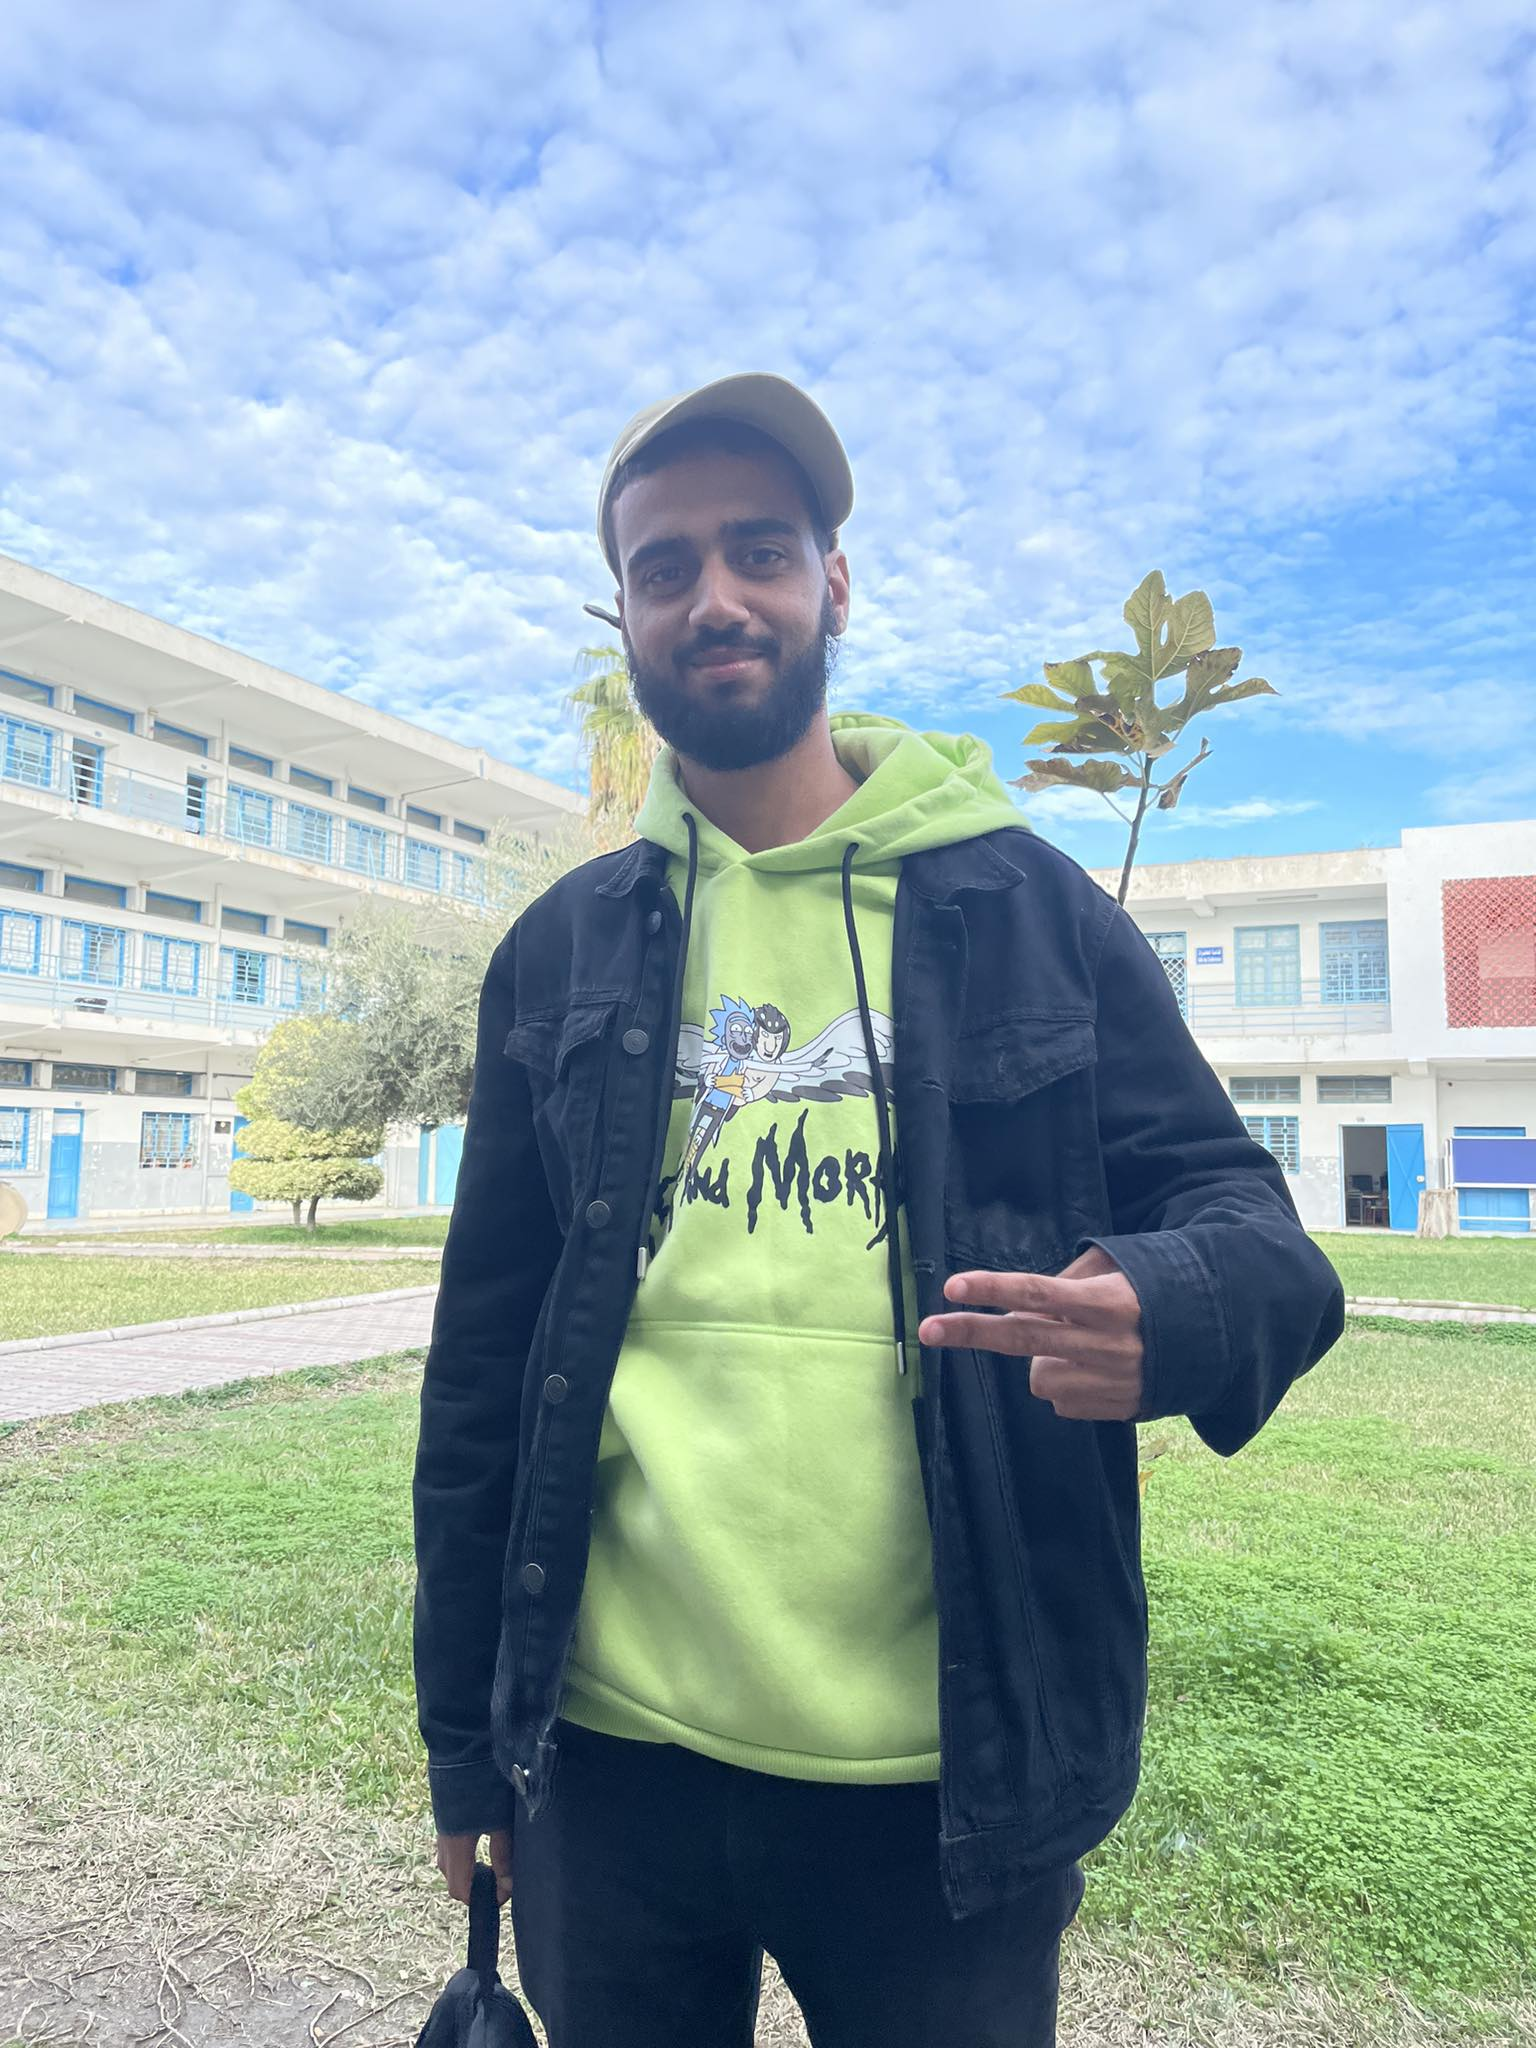
\includegraphics[width=1\textwidth]{chap1.images/binomi.jpg}
\end{figure}


\begin{figure}[p]
    \centering
    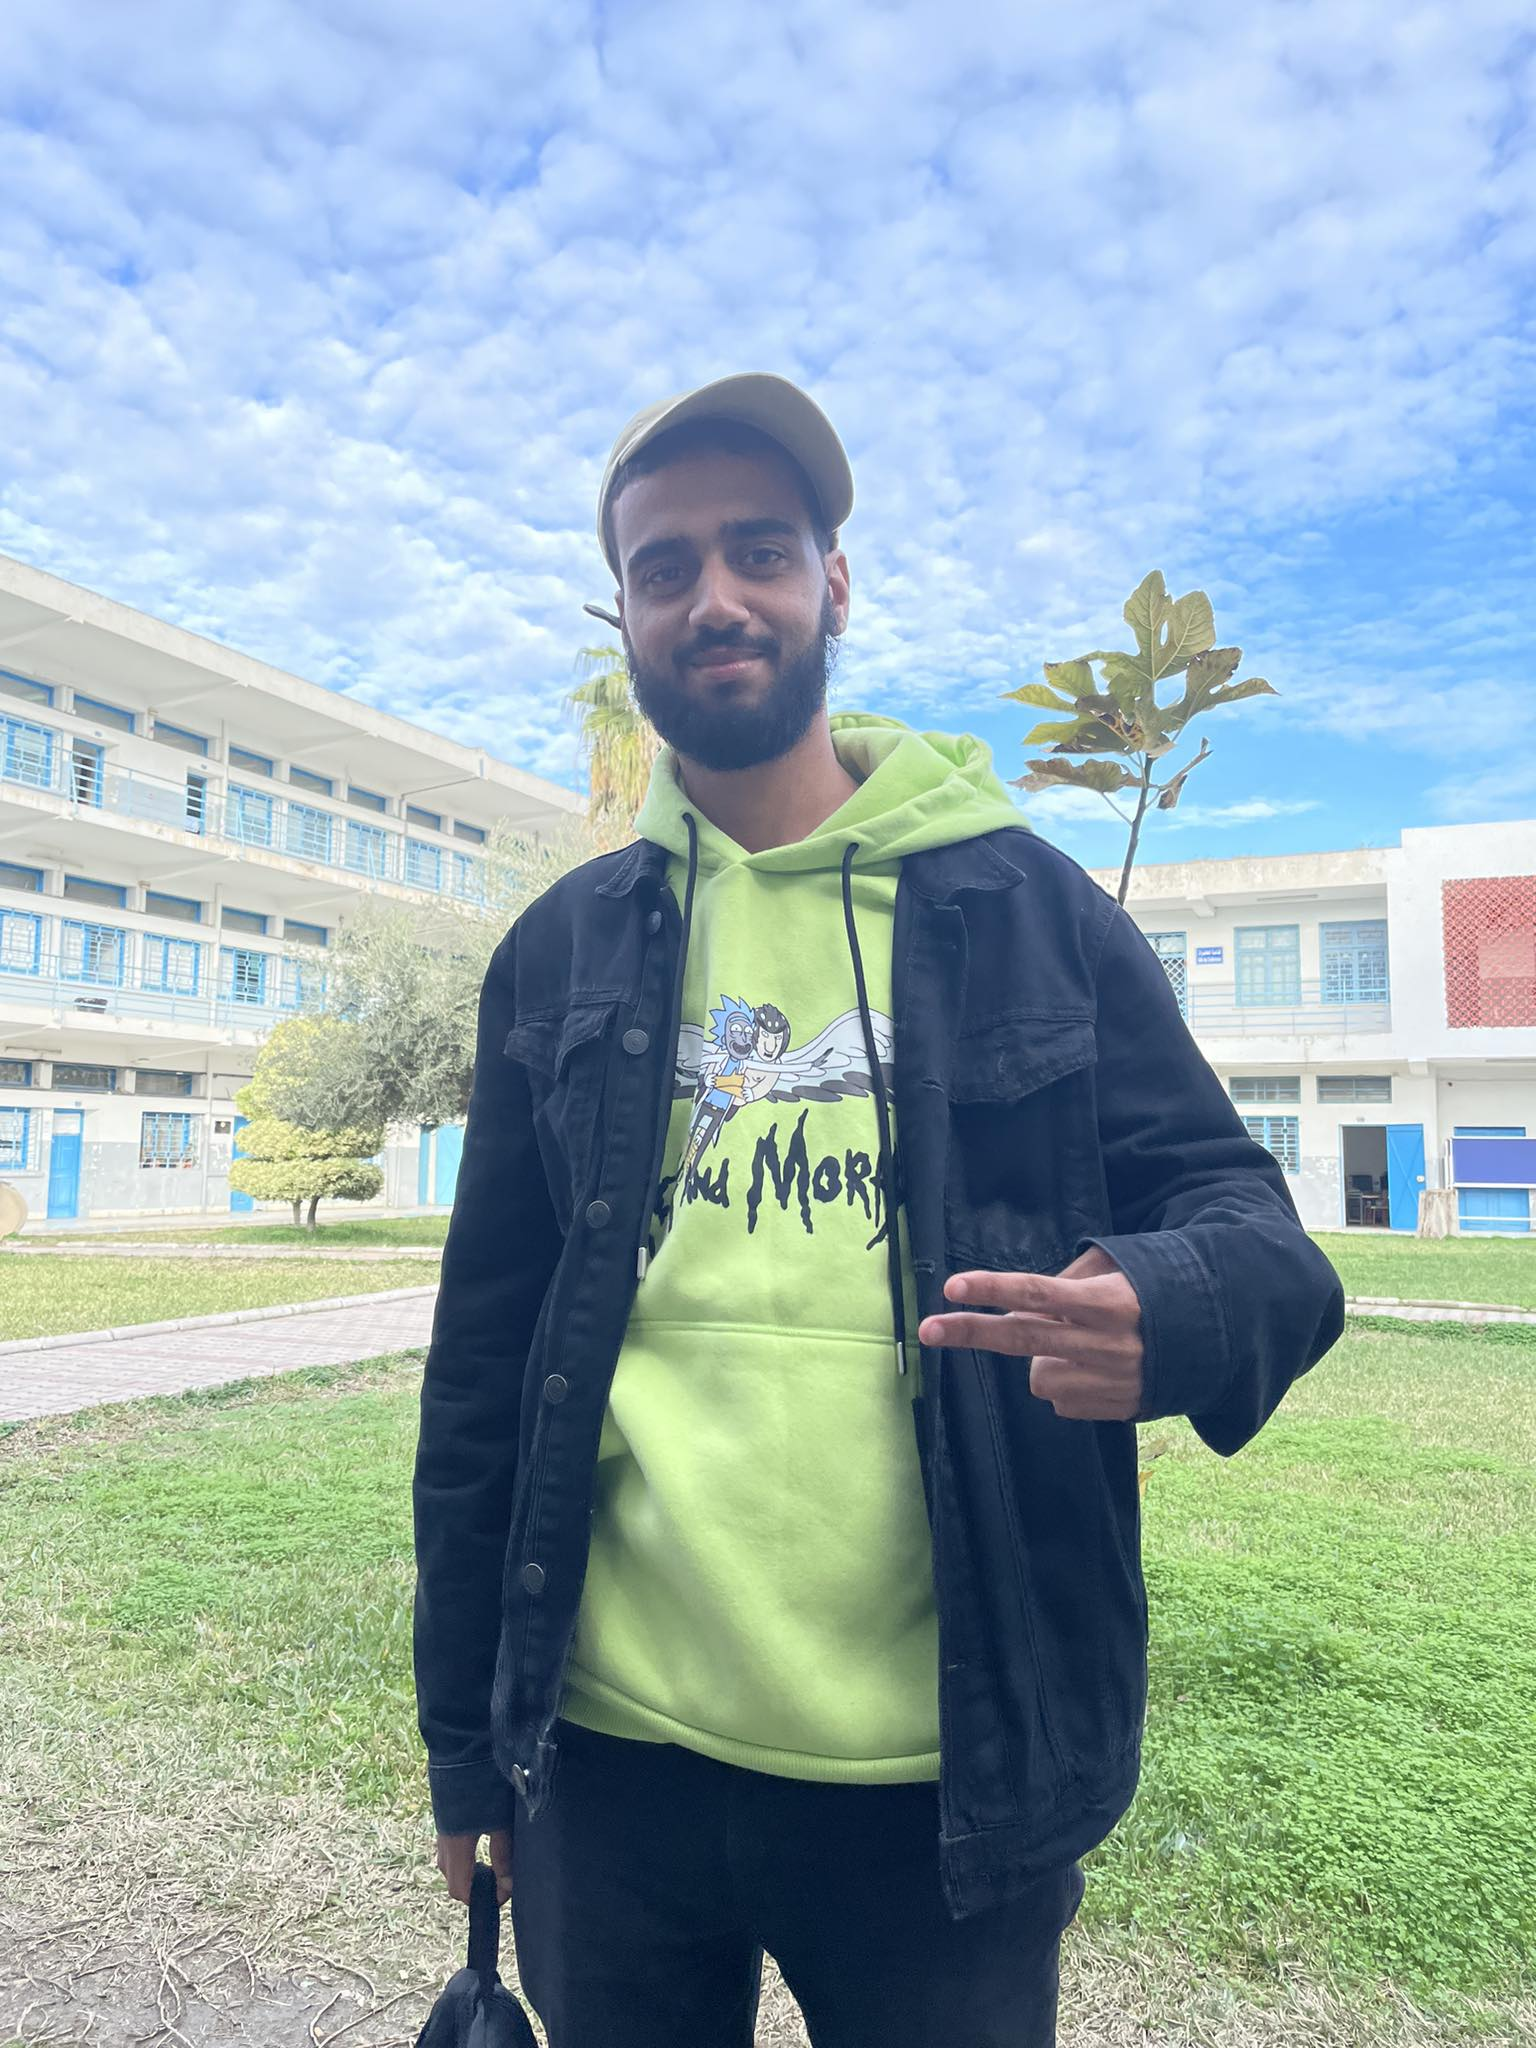
\includegraphics[width=1\textwidth]{chap1.images/binomi.jpg}
\end{figure}

\newpage



\tableofcontents
% Le package newclude mis en commentaire permet d'introduire une * pour éviter le saut de page entre les section
\pagebreak
%% Devis de recherche
\newpage
\listoffigures
\newpage
\listoftables
\newpage
\chapter*{Liste des Acronymes}

\noindent
\textbf{GMAO} : Gestion de la Maintenance Assistée par Ordinateur\newline\\
\noindent
\textbf{API} : Interface de Programmation Applicative\newline\\
\noindent
\textbf{REST} : Representational State Transfer\newline\\
\noindent
\textbf{UML} : Unified Modeling Language\newline\\
\noindent
\textbf{MVVM} : Modèle-Vue-VueModèle\newline\\
\noindent
\textbf{HTTP} : Hypertext Transfer Protocol\newline\\
\noindent
\textbf{SQL} : Structured Query Language\newline\\
\noindent
\textbf{KPI} : Key Performance Indicator \newline\\
\noindent
\textbf{ETL} : Extraction, Transformation, and Loading \newline






\input{Dedicace}
\input{Remerciement}

\chapter*{Introduction générale}
\markboth {Introduction générale}{}
\addcontentsline{toc}{chapter}{Introduction générale}


Dans le contexte actuel de la gestion d’entreprise axée sur l’efficacité opérationnelle et la rentabilité, l’optimisation des ressources et des actifs est devenue un impératif stratégique pour les organisations modernes. En effet, dans un environnement économique de plus en plus concurrentiel, les entreprises doivent non seulement maximiser l’utilisation de leurs ressources, mais également minimiser les coûts liés à leur maintenance et leur exploitation. Parmi ces actifs essentiels, les parcs d’entreprise, qu’ils comprennent des véhicules, des flottes de transport ou d’autres équipements, représentent des investissements substantiels. Ces investissements nécessitent une gestion rigoureuse et proactive pour assurer leur durabilité, leur efficacité et leur rentabilité à long terme.\\

Face à cette exigence croissante, notre projet s’attache à répondre aux besoins de gestion des parcs d’entreprise à travers le développement d’une application mobile novatrice et fonctionnelle, intégrant les principes de la GMAO (Gestion de Maintenance Assistée par Ordinateur). Cette solution numérique vise à rationaliser les processus de gestion en offrant aux parties prenantes une plateforme intégrée pour surveiller, entretenir et optimiser les parcs d’entreprise de manière efficace et transparente. L’objectif est de fournir un outil qui non seulement facilite la gestion quotidienne, mais aussi anticipe les besoins futurs grâce à des fonctionnalités avancées de suivi et d’analyse des données.\\

Dans le cadre de ce rapport, nous présentons une analyse approfondie du développement de cette application, mettant en lumière nos objectifs stratégiques, les fonctionnalités clés de l’application, ainsi que les défis rencontrés et les stratégies d’atténuation mises en œuvre. Nous détaillerons comment notre solution permet une gestion proactive grâce à des notifications automatisées pour les maintenances, des rapports détaillés sur l’utilisation et l’état des actifs, et des tableaux de bord personnalisables pour une vision claire et en temps réel des performances.\\

Nous explorerons également les implications potentielles de cette solution pour les entreprises utilisatrices, notamment en termes d’amélioration de l’efficacité opérationnelle, de réduction des coûts et d’optimisation des performances. En réduisant les temps d’arrêt des équipements et en prolongeant leur durée de vie, notre application vise à générer des économies significatives et à améliorer la productivité globale des parcs d’entreprise. De plus, en fournissant des données précises et exploitables, elle permet aux gestionnaires de prendre des décisions éclairées, d’optimiser les processus et de mieux planifier les investissements futurs.\\

Enfin, ce rapport abordera les perspectives d’évolution de notre application, avec des plans pour intégrer des améliorations continues basées sur les retours d'expérience des utilisateurs et les besoins émergents des entreprises. Notre vision est de créer une solution qui évolue avec les besoins des entreprises, offrant une flexibilité et une scalabilité pour répondre aux défis de demain.



\chapter { Etude préliminaire du projet }


\section*{Introduction}
\addcontentsline{toc}{section}{Introduction}
\bigskip
Dans le cadre de la mise en place d'une application de gestion des parking des entreprises, il est essentiel de réaliser une étude préalable approfondie afin de cerner les besoins, les contraintes et les objectifs liés à ce projet. Cette étude préalable permettra de définir les contours du projet et de poser les bases pour son développement et sa mise en œuvre.
Nous commençons par placer le projet dans son cadre général et d'exposer le contexte de travail ainsi que  les objectifs a atteindre.

%_________________________________________________________________________________________________

\section{Présentation de l’organisme d’accueil}
\bigskip
Digital Identity, connue sous l’abréviation « DIGID »est une entreprise tunisienne Fondée en 2019, spécialisée dans le conseil et le développement de solutions technologiques spécifiques à l'échelle nationale et internationale. Ses objectifs sont de permettre à ses clients de se concentrer sur leurs activités principales, en s'appuyant sur des solutions fiables et sur un partenaire crédible et inébranlable.\\
\newline DIGID est spécialisée dans le conseil et la mise en œuvre de solutions logicielles de gestion intégrée.

\bigskip
\begin{figure}[ht]
    \centering
    
\includegraphics[scale = 0.5]{chap1.images/digidlogo.png}
    \caption{Logo de l’entreprise « DIGITAL IDENTITY »}
    \label{Logo de l’entreprise « DIGITAL IDENTITY » }
\end{figure}

%____________


\newpage
\subsection{ Organigramme de l’entreprise }

L’organigramme de Digital Identity figure 1.2 présente une vue parfaite de l’oraganisation des
liens hiéarchiques entre les différentes équipes. En effet, c’est une traduction schématique des
objectifs, des missions et des relations fonctionnelles.

\begin{figure}[ht]
    \centering
    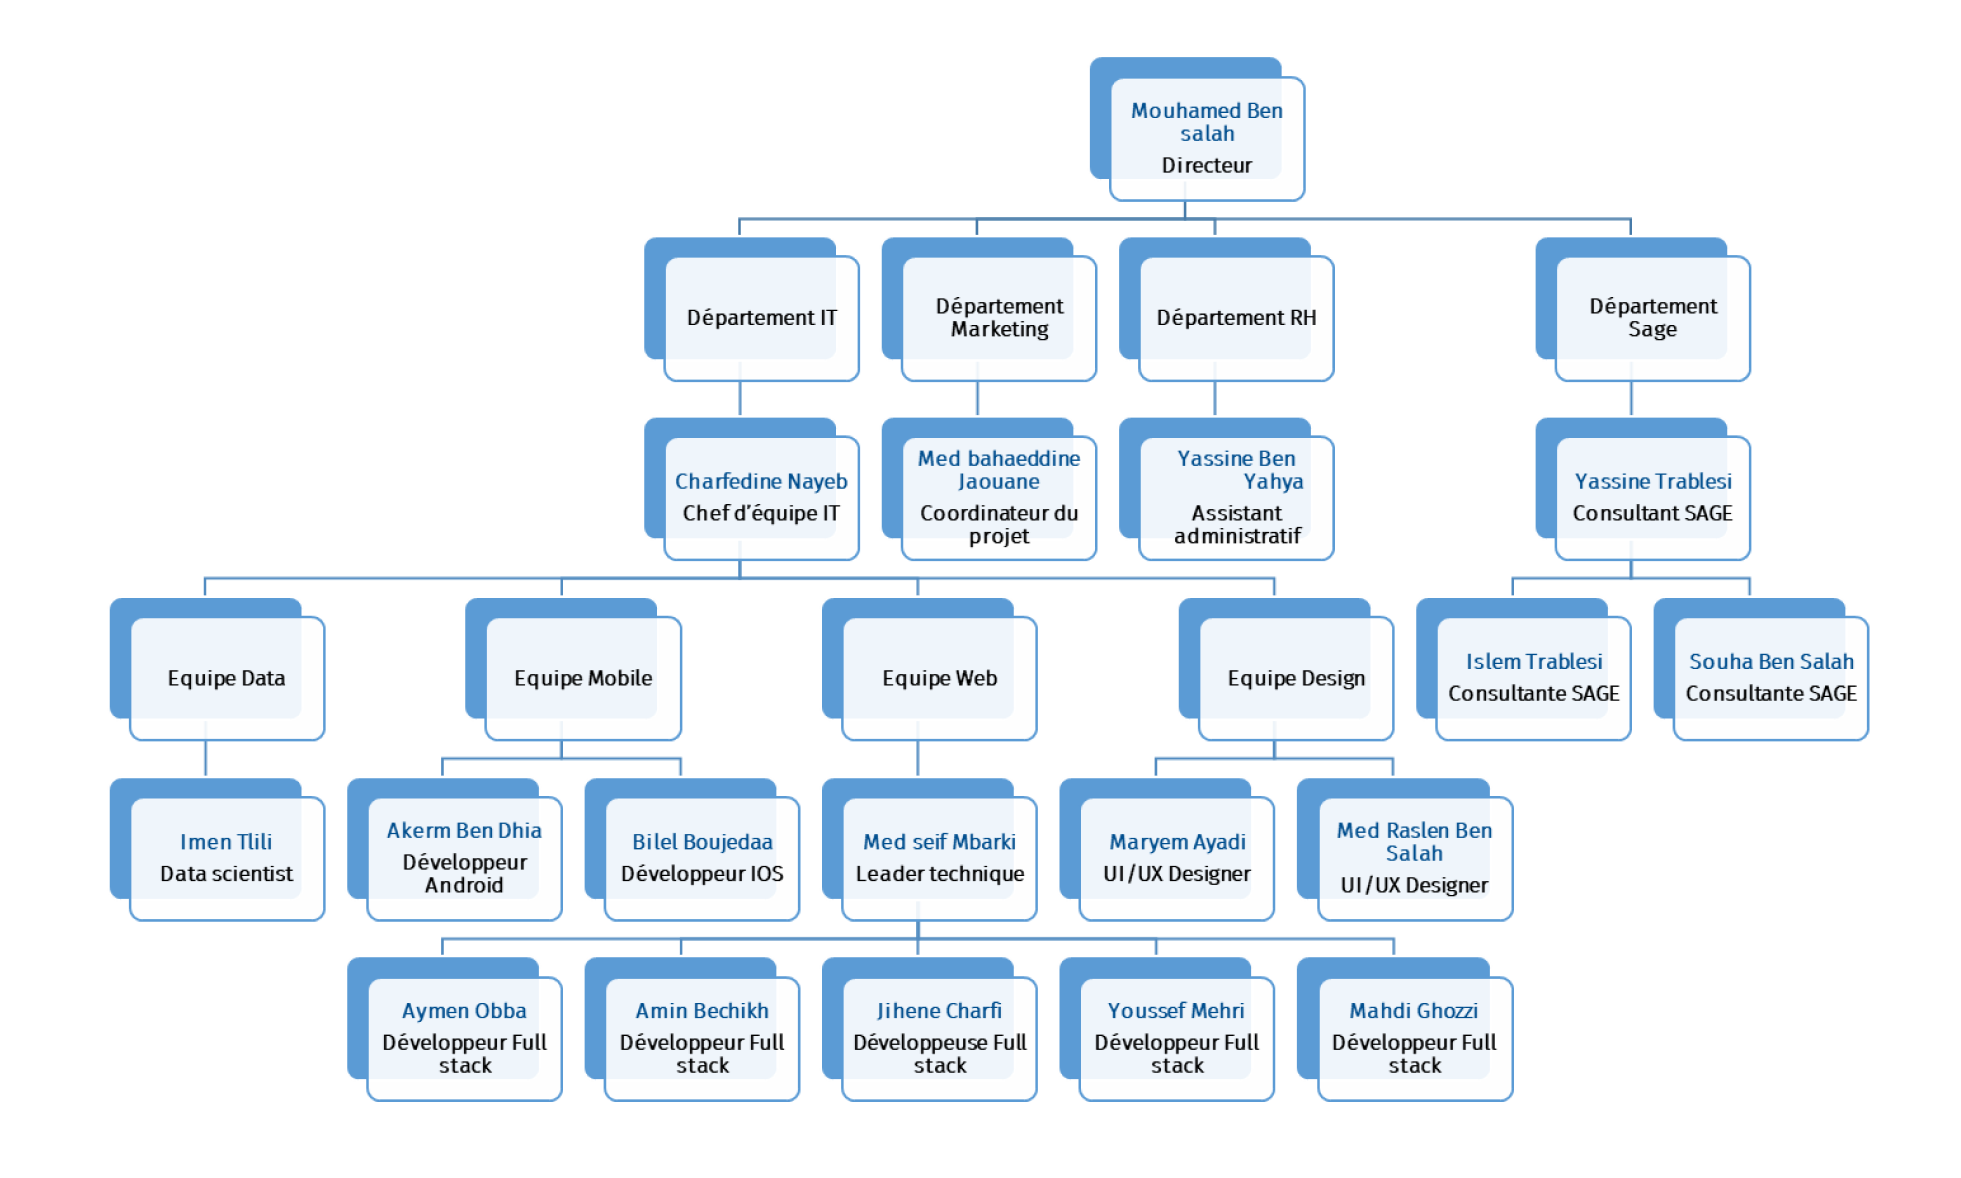
\includegraphics[width=1.1\textwidth,height=12.5cm]{chap1.images/org digid.png}
    \caption{Organigramme de Digital identity}
    \label{fig:orgcogecom}
\end{figure}


\subsection{ Les activités de Digital Identity : }
\begin{figure}[ht]
    \centering
    \includegraphics[width=1\textwidth,height=4cm]{chap1.images/digid activités.png}
    \caption{Les activités de Digital Identity}
\end{figure}
%_________________________________________________________________________________________________
\newpage
\section{Cadre du projet}
\bigskip
Dans cette section, nous allons aborder en détail la problématique soulevée et nous allons présenter une solution pertinente qui a été proposée pour y remédier.
\bigskip
\subsection{ Problématique}
\bigskip
À une époque où la gestion des parcs de véhicules d'entreprise est devenue de plus en plus complexe en raison de la diversité des véhicules, des itinéraires et des exigences opérationnelles, ainsi que des pressions technologiques et environnementales croissantes, il devient impératif de concevoir, développer et déployer une plateforme intégrée véritablement innovante et robuste pour relever ces défis multidimensionnels. Comment mettre en place une telle plateforme, capable de fournir une surveillance en temps réel, une analyse prédictive et des fonctionnalités d'optimisation avancées, tout en garantissant une efficacité opérationnelle maximale, une réduction des coûts et une durabilité environnementale accrue pour les entreprises? De plus, comment concilier ces objectifs avec les exigences de sécurité, de conformité réglementaire et de flexibilité, afin de permettre aux entreprises de prospérer dans un contexte économique en perpétuelle mutation, de maintenir leur compétitivité et d'assurer une gestion stratégique de leurs actifs de transport dans un monde en constante évolution ?



%_________________________________________________________________________________________________

\subsection{ Solution proposée}
\bigskip
Notre solution de gestion de flotte de véhicules d’entreprise repose sur une plateforme intégrée et technologiquement avancée, conçue pour répondre aux défis croissants de gestion des parcs de véhicules. Dans le cadre de cette solution, nous avons intégré une dimension Business Intelligence (BI) afin d'offrir une analyse approfondie des données et des informations stratégiques aux gestionnaires. Cette intégration du volet BI enrichit notre plateforme en lui permettant de fournir une surveillance en temps réel des véhicules, une analyse prédictive des données et des outils d'optimisation avancés.

Grâce à des tableaux de bord interactifs et des rapports personnalisables, les gestionnaires auront une vue d'ensemble précise de la performance opérationnelle de leur flotte. Ces outils leur permettront de visualiser et de suivre en temps réel des indicateurs clés de performance (KPI) tels que le taux d'utilisation des véhicules, les coûts de maintenance, les temps d'immobilisation, etc. De plus, les rapports générés par le système BI fourniront des insights stratégiques pour la prise de décision, en identifiant les tendances, les patterns et les opportunités d'optimisation.

En combinant ces fonctionnalités avancées avec une approche centrée sur les besoins des entreprises, notre solution vise à fournir une réponse complète et efficace aux défis de gestion des flottes de véhicules d’entreprise. Elle permettra aux gestionnaires de prendre des décisions éclairées et proactives pour maximiser l'efficacité opérationnelle de leur flotte, réduire les coûts associés et maintenir leur compétitivité dans un environnement commercial en constante évolution.


%______________________________________________________________________________________________




\section{Méthodologie et langage de conception}
La conception est cruciale dans le développement d'un système informatique pour répondre aux besoins du client. Les choix conceptuels concernant l'approche, le langage de modélisation et le processus de développement sont issus de réflexions collectives. Nous avons choisi la méthodologie Scrum, une méthode agile, pour réaliser notre projet.
\subsection { Méthodes agiles}
\noindent Parmi les méthodes agiles les plus couramment utilisées de nos jours, on peut citer :

\begin{itemize}[label=$\square$]
    \item Extrême Programming (XP)
    \item Scrum
    \item Agile Unified Process (Agile UP ou AUP)
\end{itemize}


Ces méthodes agiles se caractérisent par leur approche itérative et incrémentale, leur focalisation sur les besoins des utilisateurs, leur flexibilité pour répondre aux changements, leur collaboration étroite avec les parties prenantes du projet, ainsi que leur orientation vers une livraison régulière de fonctionnalités à valeur ajoutée. Chacune de ces méthodes agiles a ses propres pratiques, rôles, cérémonies et outils, mais elles partagent toutes les mêmes valeurs et principes fondamentaux de l'agilité.\\

Dans notre cas ,nous avons choisi d'adopter le framework Scrum pour le développement de notre application, car elle nous a semblé la plus adaptée à notre travail. Scrum est un framework agile qui offre une organisation flexible nous permettant de découper notre projet en plusieurs sprints. Cette approche itérative nous aidera à mieux gérer notre travail en nous concentrant sur des objectifs concrets à atteindre à chaque étape du développement.


%_________________________________________________________________________________________________


\newpage
\subsection{ Principes du framework Scrum}
Scrum est un cadre de travail pour la gestion de projet agile qui est largement utilisé à travers le monde. Il comprend des rôles bien définis, un rythme itératif, des réunions chronométrées et des artefacts tels que le product backlog, le sprint backlog et le graphique d'avancement (Burndown Chart). Ces éléments constituent les piliers du processus de gestion de projet agile offert par Scrum.\\

\begin{figure}[htbp]
    \centering
    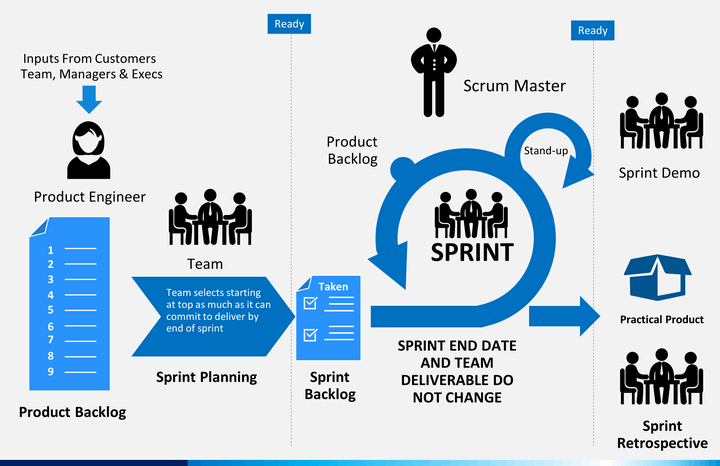
\includegraphics[width=1\textwidth]{chap1.images/scrum-process-slide2_2.png}
    \caption{Mode de fonctionnement de la méthodologie Scrum}
\end{figure}

\noindent\textbf{Sprint} : Tout projet Scrum est organisé autour de «Sprints» de développement pendant lesquels une équipe de développement travaille sur un ensemble de fonctionnalités ou d'objectifs spécifiques.

\noindent\textbf{User story} : Les fonctionnalités requises sont présentées sous la forme de "User Stories" dans une liste organisée.

\noindent\textbf{Backlog du produit} : Les user stories sont organisées dans le backlog du produit.\\

\noindent\textbf{Sprint backlog} : Le sprint backlog est une liste des éléments du product backlog sélectionnés pour être développés pendant un sprint exacte. C'est une liste de tâches à accomplir pendant le sprint. Les membres de l'équipe de développement se concentrent sur ces tâches pour les livrer à la fin du sprint.

\noindent\textbf{Planning pocker} : Pendant une réunion nommée "Réunion du Planning Poker", les user stories de chaque sprint sont estimées en points et priorisées.

\noindent\textbf{La mêlée quotidienne} : La mêlée quotidienne permet aux membres de l'équipe de se synchroniser régulièrement, de signaler rapidement les problèmes et les défis qu'ils rencontrent et de suivre l'avancement du sprint en temps réel. Cette réunion rapide et efficace est un moyen pour l'équipe de travailler de manière collaborative et d'assurer la réussite du projet.

\noindent\textbf{Revue de sprint} : L’objectif de la revue de sprint est d’inspecter l’incrément produit au cours du sprint fini.

\noindent\textbf{Rétrospective} : La rétrospective est une réunion organisée à la fin de chaque sprint pour évaluer ce qui a bien fonctionné et ce qui peut être amélioré pour le prochain sprint. L'objectif est d'améliorer continuellement les processus de travail et la collaboration de l'équipe Scrum.

%_________________________________________________________________________________________________

\subsection{ Rôles du framework Scrum}
Il existe trois rôles dans l'organisation d'un projet agile suivant la méthodologie Scrum:\\
\begin{itemize}

    \item[$\bullet$]\textbf{Product Owner: }Le Product Owner est celui qui porte la vision du produit à réaliser et travaille en interaction avec les Développeurs. Il apporte ses connaissances pour aider l'équipe de développement à comprendre les besoins et les attentes du client, tout en veillant à ce que le produit final réponde à ces exigences.\\
    \item[$\bullet$]\textbf{Scrum Master: }Le Scrum Master est un rôle clé dans le cadre de la méthode Scrum. Il est responsable de s'assurer que l'équipe Scrum suit les principes et les pratiques de Scrum. Le Scrum Master  facilite les réunions et les événements Scrum, et aide l'équipe à résoudre les obstacles ou les problèmes qui peuvent les entraver .\\
    \item[$\bullet$]\textbf{Scrum Team: }Equipe autogérée et multidisciplinaire constituée de développeurs, testeurs...  chargés de transformer les besoins exprimés par le Product Owner en fonctionnalités utilisables.
\end{itemize}
\


%_________________________________________________________________________________________________


\subsection{ Langage de modélisation}
Afin de visualiser la conception de notre système, nous avons utilisé le langage de modélisation unifié UML (Unified Modeling Language) qui permet de modéliser les besoins du logiciel à développer.

\begin{figure}[ht]
    \centering
    
\includegraphics[width=0.2\textwidth]{chap1.images/UML.png}
    \caption{UML}
\end{figure}

%______________________________________________________________________________________________
\newpage
\section{Environnement de travail}
Dans cette section, nous détaillons l'environnement de travail à savoir l'environnement matériel, l'environnement logiciel ainsi que les langages et framework utilisés.

\subsection{ Langages et framework utilisés }
\noindent Les langages et Frameworks utilisés pour l'implémentation de notre solution sont les suivants :

\begin{itemize}
    \item[$\bullet$] \textbf{ Java :}
          « C'est un Langage de programmation polyvalent et orienté objet, largement utilisé pour le développement d'applications Android et d'entreprises en raison de sa portabilité et de sa robustesse»

          \begin{figure}[ht]
              \centering 
\includegraphics[scale=0.2]{chap1.images/java.jpg}
              \caption{Java}
              \label{JAVA}
          \end{figure}



    \item[$\bullet$] \textbf{ Python :}
          « C'est un Langage de programmation populaire connu pour sa simplicité syntaxique, sa polyvalence et sa grande variété de bibliothèques, idéal pour le développement rapide d'applications, l'analyse de données et l'automatisation des tâches.»

          \begin{figure}[ht]
              \centering 
\includegraphics[scale=0.15]{chap1.images/python.jpg}
              \caption{Python}
              \label{PYTHON}
          \end{figure}



    \item[$\bullet$] \textbf{  MySQL :} « C'est un système de gestion de base de données relationnelle open source largement utilisé dans le développement d'applications web et mobiles en raison de sa fiabilité, de sa performance et de sa facilité d'utilisation. Si vous avez besoin d'assistance pour intégrer MySQL à votre application ou pour d'autres aspects de votre projet.»

          \begin{figure}[ht]
              \centering 
\includegraphics[scale=0.3]{chap1.images/MySQL.png}
              \caption{MySQL}
              \label{fig: MySQL}
          \end{figure}


    \item[$\bullet$] \textbf{ ReactJS :}
          « C'est une bibliothèque JavaScript open-source développée par Facebook pour créer des interfaces utilisateur interactives. Elle permet de construire des composants réutilisables et optimise les mises à jour de l'interface grâce au Virtual DOM.»

          \begin{figure}[ht]
              \centering 
\includegraphics[scale=0.28]{chap1.images/reactjs_logo.png}
              \caption{ReactJS}

          \end{figure}

    \item[$\bullet$] \textbf{ Node.js :}
          « C'est une plateforme d'exécution JavaScript construite sur le moteur V8 de Chrome, permettant d'exécuter du code JavaScript côté serveur. Il est réputé pour son modèle non bloquant et basé sur des événements, idéal pour des applications réseau performantes.»

          \begin{figure}[ht]
              \centering 
\includegraphics[scale=0.025]{chap1.images/Node_logo_NodeJS.png}
              \caption{Node.js}

          \end{figure}

          \bigskip
    \item[$\bullet$] \textbf{  REST API :}
          \par« Une API REST (Representational State Transfer) est une interface de programmation d'application qui utilise les méthodes HTTP standard pour permettre aux clients d'accéder et de manipuler des ressources sur un serveur. »

          \begin{figure}[ht]
              \centering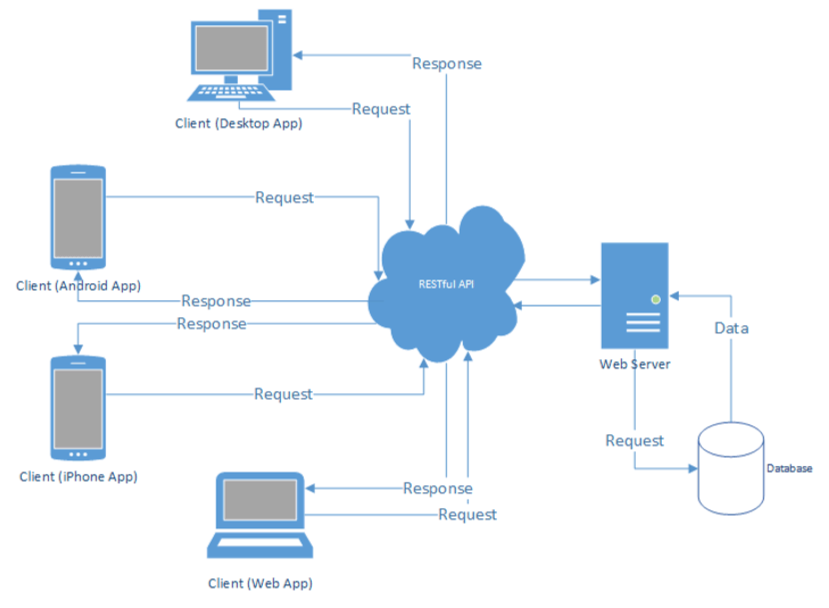
\includegraphics[scale=0.45]{chap1.images/rest-api-flow.png}
              \caption{REST API}
              \label{RESTAPI}
          \end{figure}

\end{itemize}


%__________________________________________________________________________________________________________
\newpage
\subsection{Environnement matériel}
\noindent Le tableau 1.1 montre les caractéristiques techniques des machines utilisées pour la réalisation de notre application.
\bigskip
\begin{table}[htbp]
    \renewcommand{\arraystretch}{1.9}
    \centering
    \begin{tabular}{|c|c|c|}
        \hline
        Ordinateur             & ASUS TUF F15 & ASUS TUF F15     \\
        \hline
        Propriétaire           & Balti Firas  & Mimouni Med Aziz \\
        \hline
        RAM                    & 32 GO        & 32 GO            \\
        \hline
        Processeur             & i5 11éme     & i5 11éme         \\
        \hline
        Système d’exploitation & Windows 11   & windows 11       \\
        \hline
    \end{tabular}
    \bigskip
    \caption{Description des machines de développement utilisées}

\end{table}
%____________________________________________________________________________________________
\subsection{ Environnement logiciel }

\noindent Les logiciels utilisés pour l’implémentation de notre solution sont les suivants sont les suivants :

\begin{itemize}
    \item[$\bullet$] \textbf{ Figma  :}
          C'est un outil de conception d’interface utilisateur (UI) et d’expérience utilisateur (UX) en ligne. Il permet aux designers de créer des designs d’interface utilisateur . Figma est également utilisé pour collaborer en temps réel. Nous l’avons utilisé dans notre projet pour concevoir les maquettes et les diagrammes de notre application.

          \begin{figure}[ht]
              \centering 
\includegraphics[scale=0.07]{chap1.images/FigmaLogo.png}
              \caption{Figma}
              \label{Figma}
          \end{figure}



    \item[$\bullet$] \textbf{ Android Studio :}
          C'est un environnement de développement intégré (IDE) développé par Google pour la création d’applications Android. Il est disponible gratuitement pour les développeurs Android. Nous l’avons utilisé dans notre cas pour bénéficier d’un émulateur android servant à débeuguer notre application.

          \begin{figure}[ht]
              \centering 
\includegraphics[scale=0.3]{chap1.images/andoird studio.png}
              \caption{Android Studio}
              \label{Android Studio}
          \end{figure}



    \item[$\bullet$] \textbf{  Overleaf :}
          C'est un éditeur en ligne de LaTeX, un langage de composition de documents scientifiques et techniques. Il permet aux utilisateurs de créer, de modifier et de collaborer sur des documents LaTeX en temps réel, Tout au long de notre stage de projet de fin d’étude, nous l’avons utilisé pour travailler ensemble sur un seul document et suivre les modifications apportées par chacune de nous en temps réel.

          \begin{figure}[h]
              \centering 
\includegraphics[scale=0.14]{chap1.images/overleaflogo.png}
              \caption{Overleaf}
              \label{fig: Overleaf}
          \end{figure}


          \bigskip
    \item[$\bullet$] \textbf{  Spyder :}
          C'est un environnement de développement interactif (IDE) spécialement conçu pour Python, offrant une interface conviviale et des fonctionnalités avancées telles que l'édition de code, l'exploration de variables et la gestion de projets. Nous avons choisi d'utiliser Spyder dans notre cas pour sa simplicité d'utilisation et sa compatibilité avec Python, ce qui nous a permis de développer et de déboguer efficacement notre code .


          \begin{figure}[ht]
              \centering
\includegraphics[scale=0.3]{chap1.images/spyder_logo.png}
              \caption{Spyder}
              \label{Spyder}
          \end{figure}
          \bigskip
    \item[$\bullet$] \textbf{  Jira :}
          C'est un outil de gestion de projet, conçu pour aider les équipes à planifier, suivre et gérer leurs tâches et leurs projets. Il offre une interface conviviale pour la création de backlogs, l'attribution de tâches, le suivi des progrès et la gestion des délais. Grâce à ses fonctionnalités de collaboration , Jira permet aux équipes de travailler de manière coordonnée et de respecter les délais de manière transparent.

          \begin{figure}[H]
              \centering
\includegraphics[scale=0.2]{chap1.images/jira-logo.png}
              \caption{Jira}

          \end{figure}

          \newpage

    \item[$\bullet$] \textbf{  Slack :}
          C'est une plateforme de communication collaborative propriétaire (SaaS). Nous avons utilisé Slack lors de notre période de stage pour assurer et faciliter la communication avec l’équipe de l’entreprise d’acceuil.

          \begin{figure}[ht]
              \centering
\includegraphics[scale=0.22]{chap1.images/Slack.logo.png}
              \caption{Slack}

          \end{figure}



    \item[$\bullet$] \textbf{  Material UI :}
          C'est une bibliothèque de composants React qui facilite la création d'interfaces utilisateurs avec des éléments préconçus basés sur les principes du Material Design de Google. Elle permet une personnalisation poussée et un développement rapide.
          \bigskip
          \begin{figure}[ht]
              \centering
\includegraphics[width=0.15\textwidth,height=1.8cm]{chap1.images/material-ui-logo.png}
              \caption{Material UI}

          \end{figure}

    \item[$\bullet$] \textbf{ Visme :}
          C'une plateforme de création visuelle en ligne,  nous avons utilisé cette outil pour la création de nos burndown charts.

          \begin{figure}[ht]
              \centering
\includegraphics[scale=0.3]{chap1.images/vismelogo.jpg}
              \caption{Visme}
          \end{figure}


    \item[$\bullet$] \textbf{ Postman :}
          C'est un outil qui simplifie le test et le développement d'API en permettant d'envoyer des requêtes HTTP et d'analyser les réponses via une interface utilisateur conviviale.

          \begin{figure}[H]
              \centering
\includegraphics[scale=0.28]{chap1.images/Postman-Logo.jpg}
              \caption{Postman}

          \end{figure}




\end{itemize}
%_________________________________________________________________________________________________________
%____________________________________________________________________________________________________________


\newpage
\section{Organisation du travail}

Pour assurer une organisation optimale tout au long du développement de notre projet, nous avons mis en place une série de processus et de pratiques collaboratives. Nous avons débuté par des séances de brainstorming, où nous avons généré et partagé des idées. Ces propositions ont ensuite été soumises à des réunions quotidiennes avec notre encadrant professionnel pour validation et conseils. En parallèle, nous avons consulté notre encadrant académique pour le filtrage et le développement des idées. Une fois la phase de conception achevée, nous avons entamé la création du backlog sur Jira, ce qui nous a permis de planifier et d'organiser efficacement les différentes tâches à réaliser. Ensuite, nous avons progressé vers la phase de codage.\\

\begin{figure}[ht]
    \centering
    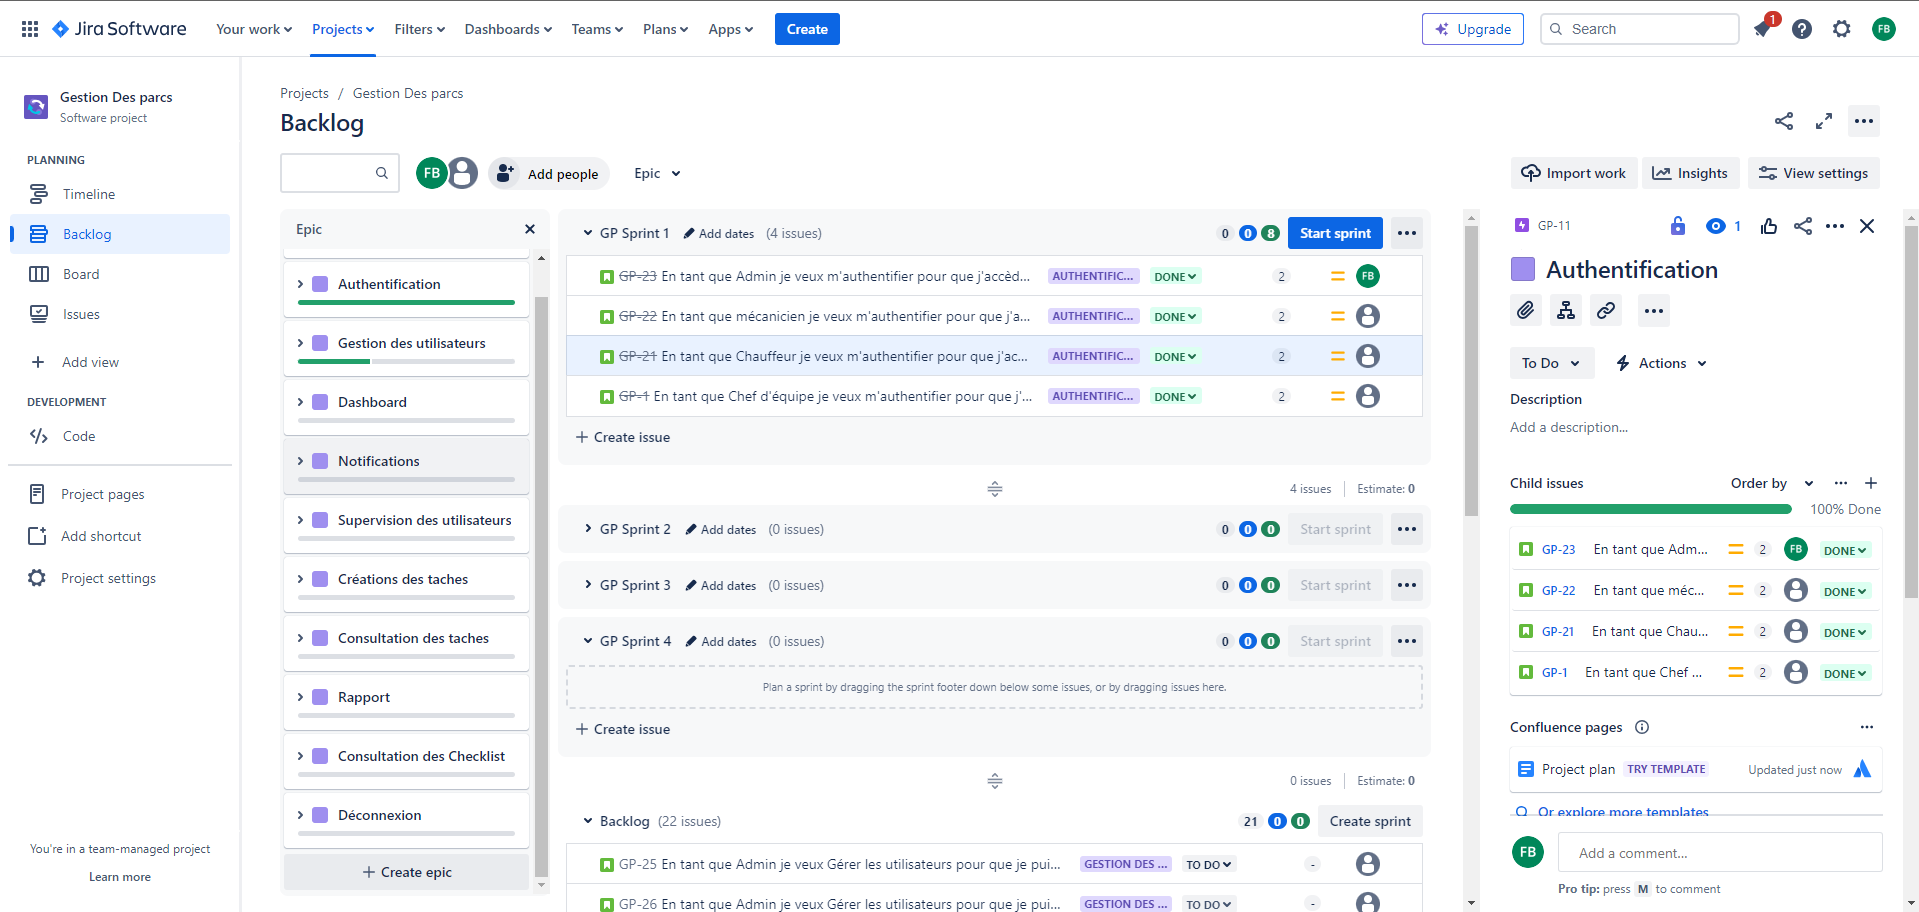
\includegraphics[width=0.85\textwidth]{chap1.images/jira.png}
    \caption{Création du backlog avec Jira}
\end{figure}

Pour faciliter la collaboration et le partage du code en temps réel, nous avons opté pour l'utilisation de GitHub. Chacun de nous a pu "pusher" ses changements une fois les tâches accomplies, ce qui nous a permis de suivre l'avancement de chacun et de garantir le respect des délais de réalisation de nos sprints. \\
\begin{figure}[ht]
    \centering
    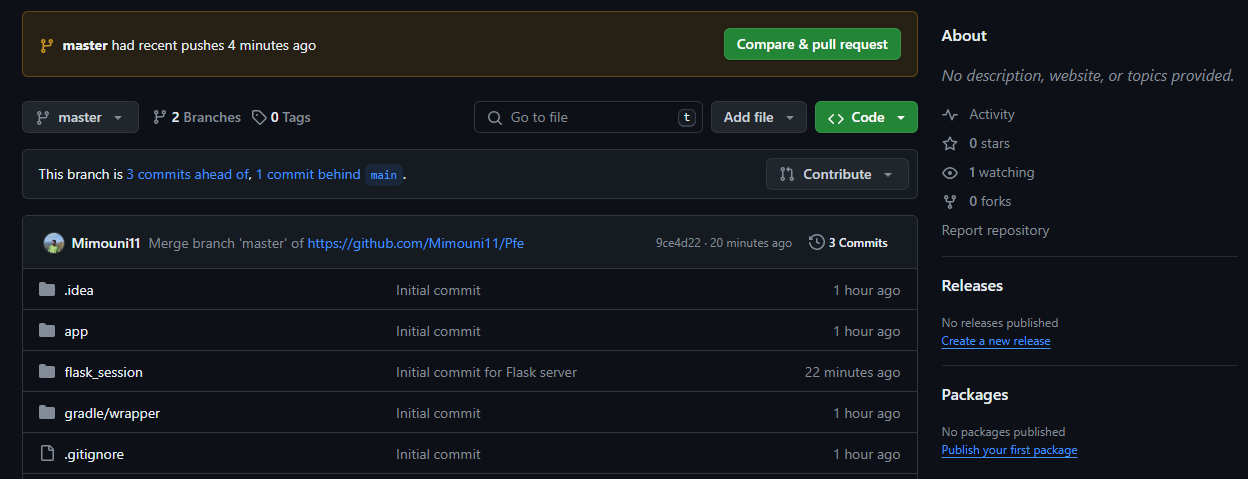
\includegraphics[width=0.85\textwidth]{chap1.images/depot git.png}

    \caption{Dépôt GitHub}
\end{figure}


%_____________________________________________________________________________________________________


\newpage
\section*{Conclusion}
\addcontentsline{toc}{section}{Conclusion}
\bigskip
\begin{sloppypar}
    Dans ce chapitre, nous avons introduit l’organisme d’accueil, clarifié le cadre du projet  et décrit les choix méthodologiques ainsi que l’architecture. Le prochain chapitre se concentrera sur la planification du projet et la définition des fonctionnalités de l’application
\end{sloppypar}









\chapter{ Planification du projet}


\addcontentsline{toc}{section}{Introduction}

Ce chapitre a pour objectif de présenter les différents acteurs impliqués dans le projet, les besoins fonctionnels et non fonctionnels  requis par le client, ainsi que le backlog du produit. En d'autres termes, nous allons fournir une vue d'ensemble des éléments clés nécessaires pour comprendre le projet dans son ensemble.
\section{Spécification des besoins}
Dans cette partie du chapitre, nous allons spécifier les différents acteurs et les divers besoins fonctionnels et non fonctionnels de notre application.
\subsection{Identification des acteurs}
Cette étape vise à identifier les acteurs interagissant directement avec le système étudié. Un acteur représente un rôle joué par une entité externe, pouvant être un utilisateur humain, un dispositif matériel ou un autre système. Notre système est destiné à être utilisé par quatre profils d'acteurs. La figure 2.1 présente les acteurs dans notre application :




\begin{itemize}

  \item[$\bullet$] \textbf {Administrateur:} L'administrateur est responsable de la gestion globale du système. Il a des privilèges étendus, y compris la configuration du système, la gestion des utilisateurs et des autorisations, ainsi que la surveillance et la maintenance du système dans son ensemble. \\

  \item[$\bullet$] \textbf{Chef d'équipe:} Le chef d'équipe supervise à la fois les chauffeurs et les mécaniciens, assurant ainsi la coordination efficace des opérations sur le terrain et dans l'atelier. Il utilise l'application pour assigner des tâches, suivre les progrès des chauffeurs et des mécaniciens, gérer les horaires et les itinéraires, ainsi que pour recevoir des alertes sur les problèmes ou les retards. \\

  \item[$\bullet$] \textbf{Chauffeur:} Le chauffeur est l'utilisateur chargé de conduire les véhicules de l'entreprise pour effectuer diverses tâches, telles que le transport de marchandises ou la réalisation de missions spécifiques. Il utilise l'application pour signaler son statut, ses itinéraires, et pour recevoir des notifications sur les tâches à effectuer. \\

  \item[$\bullet$] \textbf {Mécanicien:} Le mécanicien est chargé de la maintenance et de la réparation des véhicules de l'entreprise. Il utilise l'application pour signaler les problèmes, demander des pièces de rechange, et pour recevoir des tâches de maintenance préventive ou corrective.\\

\end{itemize}

\begin{figure}[ht!]
  \centering
  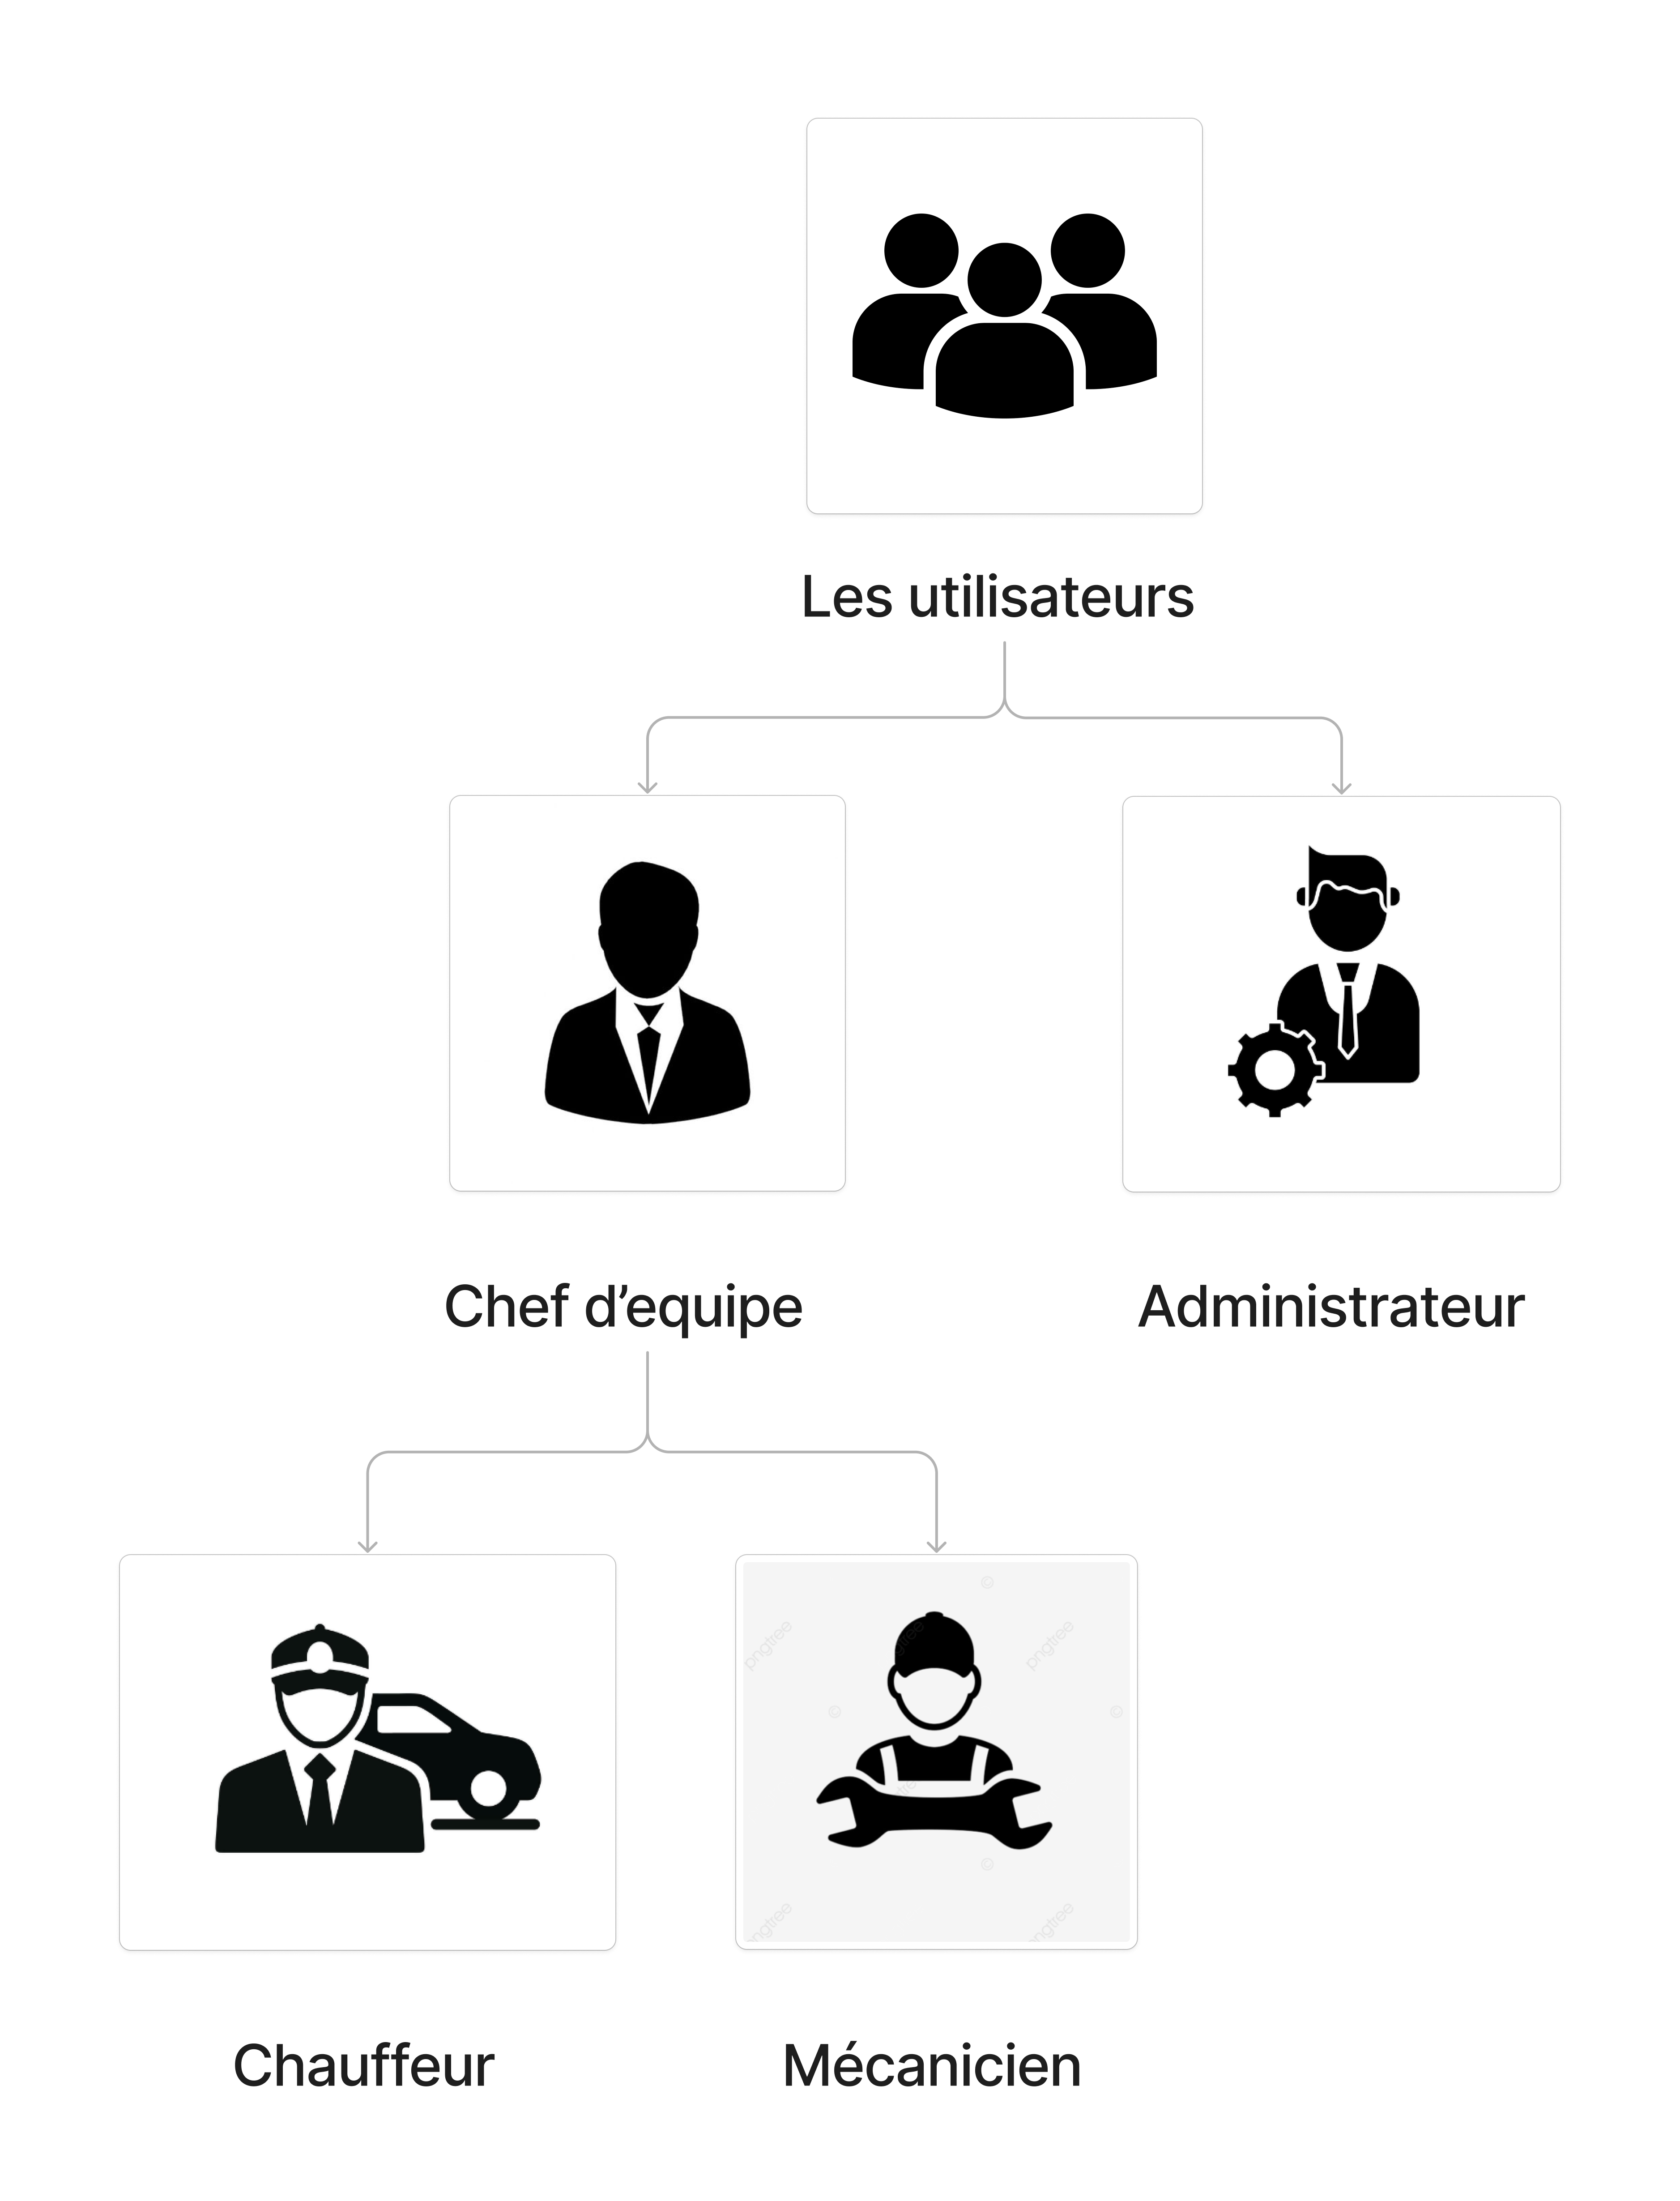
\includegraphics[width=0.7\textwidth,height=12cm]{chap2.images/Diagramme des acteurs.png}
  \caption{Diagramme des acteurs}
\end{figure}

%________________________________________________________________________________________________________




%__________________________________________________________________________________________________________

\newpage
\subsection{Besoins fonctionnels}
La spécification des besoins fonctionnels détermine les exigences fonctionnelles ainsi que les principaux objectifs et fonctionnalités de l'application. En d'autres termes, elle spécifie ce que le système étudié doit faire.\\

\begin{itemize}


  \item[$\bullet$] \textbf {S’authentifier:} Toute personne inscrite devra s’authentifier en saisissant son nom d’utilisateur ainsi que son mot de passe afin d’accéder aux fonctionnalités du statut sous lequelle elle est inscrite.\\

  \item[$\bullet$] \textbf {Gérer profil:} Chaque acteur qu’il soit administrateur, chef d'equipe, chauffeur ou même mécanicien peut gérer son propre compte.\\

  \item[$\bullet$] \textbf {Gestion des utilisateurs :} Permet à l’administrateur de gérer les comptes des utilisateurs de l’application, y compris la création, la modification et la suppression des comptes. Lors de la création d'un utilisateur (chef d'équipe, chauffeur ou mécanicien), un email contenant les paramètres de connexion ainsi qu'un manuel d'utilisation de l'application en PDF, adapté à chaque type d'utilisateur, sera envoyé automatiquement.\\

  \item[$\bullet$] \textbf {Gestion des rôles :}  Permet à l'administrateur d'attribuer des rôles spécifiques à chaque utilisateur, déterminant ainsi leurs permissions et leurs accès au système.\\

  \item[$\bullet$] \textbf {Gestion des Véhicules :} L'administrateur peut ajouter de nouveaux véhicules, supprimer des véhicules existants et visualiser la liste complète des véhicules dans le système .\\

  \item[$\bullet$] \textbf {Notifications :} Les notifications sont catégorisées (accidents, maintenance, demande de pièce ...) pour une gestion proactive des événements.\\

  \item[$\bullet$] \textbf {Création des tâches :} Permet à l'administrateur de créer, attribuer, suivre et gérer les tâches assignées aux chauffeurs, mécaniciens et chefs d'équipe. \\

  \item[$\bullet$] \textbf {Suivi des tâches :} Permet au chef d'équipe de suivre l'état et la progression des tâches assignées à son équipe, en vérifiant leur avancement et en s'assurant de leur complétion.\\

  \item[$\bullet$] \textbf {Surveillance en temps réel des déplacements des véhicules :} Donne au chef d'équipe la capacité de surveiller les déplacements en temps réel des véhicules de l'entreprise, afin de coordonner efficacement les opérations.\\

  \item[$\bullet$] \textbf {Consultation de checklist :} Permet au chauffeur de consulter les listes de vérification nécessaires avant de commencer un voyage ou une mission, garantissant ainsi la conformité et la sécurité .\\

  \item[$\bullet$] \textbf {Planification des voyages :} Autorise le chauffeur à planifier ses itinéraires et ses voyages à l'avance, en tenant compte des horaires, des destinations et d'autres paramètres pertinents. \\

  \item[$\bullet$] \textbf {Confirmation des tâches :} Permet au chauffeur de confirmer la réalisation des tâches qui lui sont assignées, telles que la livraison de marchandises ou la maintenance préventive des véhicules.\\

  \item[$\bullet$] \textbf {Consultation des tâches :} Donne au mécanicien la possibilité de consulter les tâches de maintenance assignées, y compris les réparations à effectuer et les inspections à réaliser..\\

  \item[$\bullet$] \textbf {Rapport :}  Permet au mécanicien de générer des rapports détaillés sur les travaux effectués, les pièces utilisées et l'état général des véhicules, contribuant ainsi à la gestion proactive de la maintenance.\\


\end{itemize}


%__________________________________________________________________________________________________________


\subsection{Besoins non fonctionnels}
La définition des besoins non fonctionnels est cruciale pour déterminer les caractéristiques et la qualité requises du système. Ils n’affectent pas directement les fonctionnalités de l'application, mais peuvent avoir un impact sur sa performance et son efficacité globale. Il est important de ne pas les négliger lors de la conception et du développement de l'application. Les principaux besoins non fonctionnels de cette application sont:

\begin{itemize}
  \item[$\bullet$] \textbf {Simplicité d'utilisation}:  Assurer une interface utilisateur intuitive et conviviale pour toutes les catégories d'utilisateurs, minimisant ainsi la courbe d'apprentissage et favorisant l'adoption de l'application.\\

  \item[$\bullet$] \textbf {Sécurité des données}: Assurer la confidentialité, l'intégrité et la disponibilité des données sensibles telles que les informations sur les véhicules, les tâches et les utilisateurs.\\

  \item[$\bullet$] \textbf {Évolutivité}: Concevoir l'application pour qu'elle puisse s'adapter à l'augmentation du nombre d'utilisateurs, de véhicules et de fonctionnalités sans compromettre les performances ou la fiabilité du système.\\

  \item[$\bullet$] \textbf {Disponibilité}:  Assurer la disponibilité continue de l'application, minimisant ainsi les temps d'arrêt et les interruptions des opérations.


\end{itemize}


%__________________________________________________________________________________________________________


\newpage
\subsection{Diagramme de cas d'utilisation}
La figure 2.2 illustre le diagramme de cas d'utilisation géneral de notre application.
\begin{figure}[ht]
  \centering
  \includegraphics[width=1\textwidth,height=18cm]{chap2.images/use case global.png}
  \caption{Diagramme de cas d'utilisation global}
\end{figure}



%__________________________________________________________________________________________________________



\newpage
\section{Pilotage du projet avec Scrum}
Cette section comportant l’équipe du projet et ses rôles, le backlog du produit et le découpage du projet en sprint, présente le pilotage du projet avec Scrum .
\subsection{Équipe et rôles}
L'équipe responsable du pilotage du projet est composée de:\\
\begin{itemize}
  \item[$\bullet$]\textbf{Product owner: } Digital Identity.\\
  \item[$\bullet$]\textbf{Scrum master: } C'est un membre de l'équipe de développement de Digid Mr Baha jaouane . \\
  \item[$\bullet$]\textbf{Scrum team: }C'est l'équipe de développement qui englobe nous mêmes Mimouni med aziz  et Balti firas. \\
\end{itemize}
\subsection{Contraintes et exigences}
La réussite du développement et de l'implémentation d'une solution technique dépend de l'identification des besoins réels des parties prenantes. Certaines fonctionnalités et besoins sont plus importants que d'autres, et il est crucial de les réaliser en premier pour assurer la continuité et la clarté de l'application. Pour cela, il est essentiel d'établir un ordre de priorité afin de coordonner les tâches à effectuer. Ce processus implique de classer les besoins en trois catégories selon leur importance : élevée, moyenne et faible, tout au long du cycle de vie de la solution technique.
\subsection{Risques}
Les principaux obstacles qui peuvent entraver notre progression sont la complexité de l'application et les exigences à respecter. Il est également important de prendre en compte la représentation des fonctionnalités similaires au cours de deux sprints consécutifs, afin d'éviter toute redondance inutile. Pour minimiser les risques, il est donc préférable de regrouper ces fonctionnalités similaires ensemble, plutôt que de les aborder séparément.
\subsection{Backlog du produit}
Le backlog du produit (Table 2.1) montre la liste des exigences et des fonctionnalités qui doivent être réalisées pour un produit donné ainsi que leurs degrés de priorité et de risque. Il sert de document de référence pour l'équipe de développement, les parties prenantes et les clients, afin de s'assurer que les travaux sont bien alignés sur les objectifs du projet et les besoins des utilisateurs finaux.



%______________________________________________________________________________________________________







\begin{table}[htbp]
  \centering
  \renewcommand{\arraystretch}{4.15} % Facteur d'étirement des lignes
  \begin{tabular}{|c|c|c|c|}
    \hline
    \textbf{ID}   & \textbf{USER STORIES}                                                                                                                                                            & \textbf{PRIORITE} & \textbf{RISQUE} \\

    %%%%%%%%%%%%%%%%%%%%%%%%%%%%%%%%%%%%%%%%%%%%%%%%%%%%%%%%%%%%%%        

    \hline
    \textbf{US1}  & \parbox{9cm}{\centering En tant qu’administrateur,, chauffeur, chef d'équipe et mécanicien je veux m'authentifier pour que j'accède a mon espace.}                               & Elevée            & Faible          \\
    \hline
    \textbf{US2}  & \parbox{9cm}{\centering En tant qu’administrateur,, chauffeur, chef d'équipe et mécanicien je veux me déconnecter pour que je quitte l'application.}                             & Elevée            & Faible          \\
    \hline
    \textbf{US3}  & \parbox{9cm}{\centering En tant qu’administrateur,, chauffeur, chef d'équipe et mécanicien je veux modifier mon profil.}                                                         & Elevée            & Faible          \\
    \hline
    \textbf{US4}  & \parbox{9cm}{\centering En tant qu'administrateur, je veux pouvoir gérer les rôles des utilisateurs, afin de contrôler l'accès aux fonctionnalités de l'application}             & Elevée            & Faible          \\
    \hline
    \textbf{US5}  & \parbox{9cm}{\centering En tant qu'administrateur, je veux ajouter, supprimer et  visualiser les véhicules .}                                                                    & Elevée            & Faible          \\
    \hline
    \textbf{US6}  & \parbox{9cm}{\centering En tant qu’administrateur, je veux Gérer les utilisateurs pour que je puisse ajouter/modifier/supprimer des utilisateurs. }                              & Elevée            & Faible          \\


    %%%%%%%%%%%%%%%%%%%%%%%%%%%%%%%%%%%%%%%%%%%%%%%%%%%%%%%%%%%%%%

    \hline
    \textbf{US7}  & \parbox{9cm}{\centering En tant que Chef d'équipe je veux suivre le progrès et la localisation des voiture .}                                                                    & Elevée            & Faible          \\
    \hline
    \textbf{US8}  & \parbox{9cm}{\centering En tant que Chef d'équipe je veux Créer des taches pour les chauffeurs et les mécanicien .}                                                              & Elevée            & Faible          \\
    \hline
    \textbf{US9}  & \parbox{9cm}{\centering En tant que Mécanicien je veux Consulter les détails des interventions .}                                                                                & Elevée            & Faible          \\
    \hline
    \textbf{US10} & \parbox{9cm}{\centering En tant que Chauffeur je veux consulter la checklist avant et aprés le départ . }                                                                        & Elevée            & Faible          \\

    %%%%%%%%%%%%%%%%%%%%%%%%%%%%%%%%%%%%%%%%%%%%%%%%%%%%%%%%%%%%%%

    \hline
    \textbf{US11} & \parbox{9cm}{\centering En tant qu’administrateur, chauffeur, mécanicien ou chef d’équipe, je veux recevoir des notifications pour être informé en temps réel des mises à jour.} & Elevée            & Faible          \\
    \hline
  \end{tabular}
\end{table}




%%%%%%%%%%%%%%%%%%%%%%%%%%%%%%%%%%%%%%%%%%%%%%%%%%%%%%%%%%%%%%
\begin{table}[htbp]
  \centering
  \renewcommand{\arraystretch}{4.15} % Facteur d'étirement des lignes
  \begin{tabular}{|c|c|c|c|}

    \hline
    \textbf{US12} & \parbox{11cm}{\centering En tant que Mécanicien je veux Générer des rapports pour que je puisse documenter les détails de chaque intervention.}                                       & Elevée & Faible \\
    \hline
    \textbf{US13} & \parbox{11cm}{\centering En tant qu’administrateur, je veux avoir accès à un tableau de bord pour que je puisse superviser l'ensemble des opérations.}                                & Elevée & Faible \\
    \hline
    \textbf{US14} & \parbox{11cm}{\centering En tant que Chef d'équipe, je veux un tableau de bord pour suivre les déplacements en temps réel des chauffeurs et gérer les missions de manière proactive.} & Elevée & Faible \\
    \hline
    \textbf{US15} & \parbox{11cm}{\centering En tant que Chauffeur je veux Consulter un tableau de bord pour que je puisse avoir une vue claire de mes missions actuelles}                                & Elevée & Faible \\
    \hline
    \textbf{US16} & \parbox{11cm}{\centering En tant que Mécanicien, je veux consulter un tableau de bord pour avoir une vue d'ensemble des opérations de maintenance.}                                   & Elevée & Faible \\
    \hline
  \end{tabular}
  \bigskip
  \caption{Backlog du produit}
  \label{tab:my_label}
\end{table}




%______________________________________________________________________________________________


\newpage{}
\section{Conception de l'application}

Dans cette section, nous présentons les prototypes de l'applications , la charte graphique, le plan de l'application ainsi que le diagramme de classes du domaine et le diagramme de gantt.

\subsection{Prototypes de l'application}


Les figure 2.3 et 2.4 illustrent les ecrans de chargement dans l'application.

\begin{figure}[h!]
  \centering
  \begin{minipage}[t]{0.60\textwidth}
    \centering
    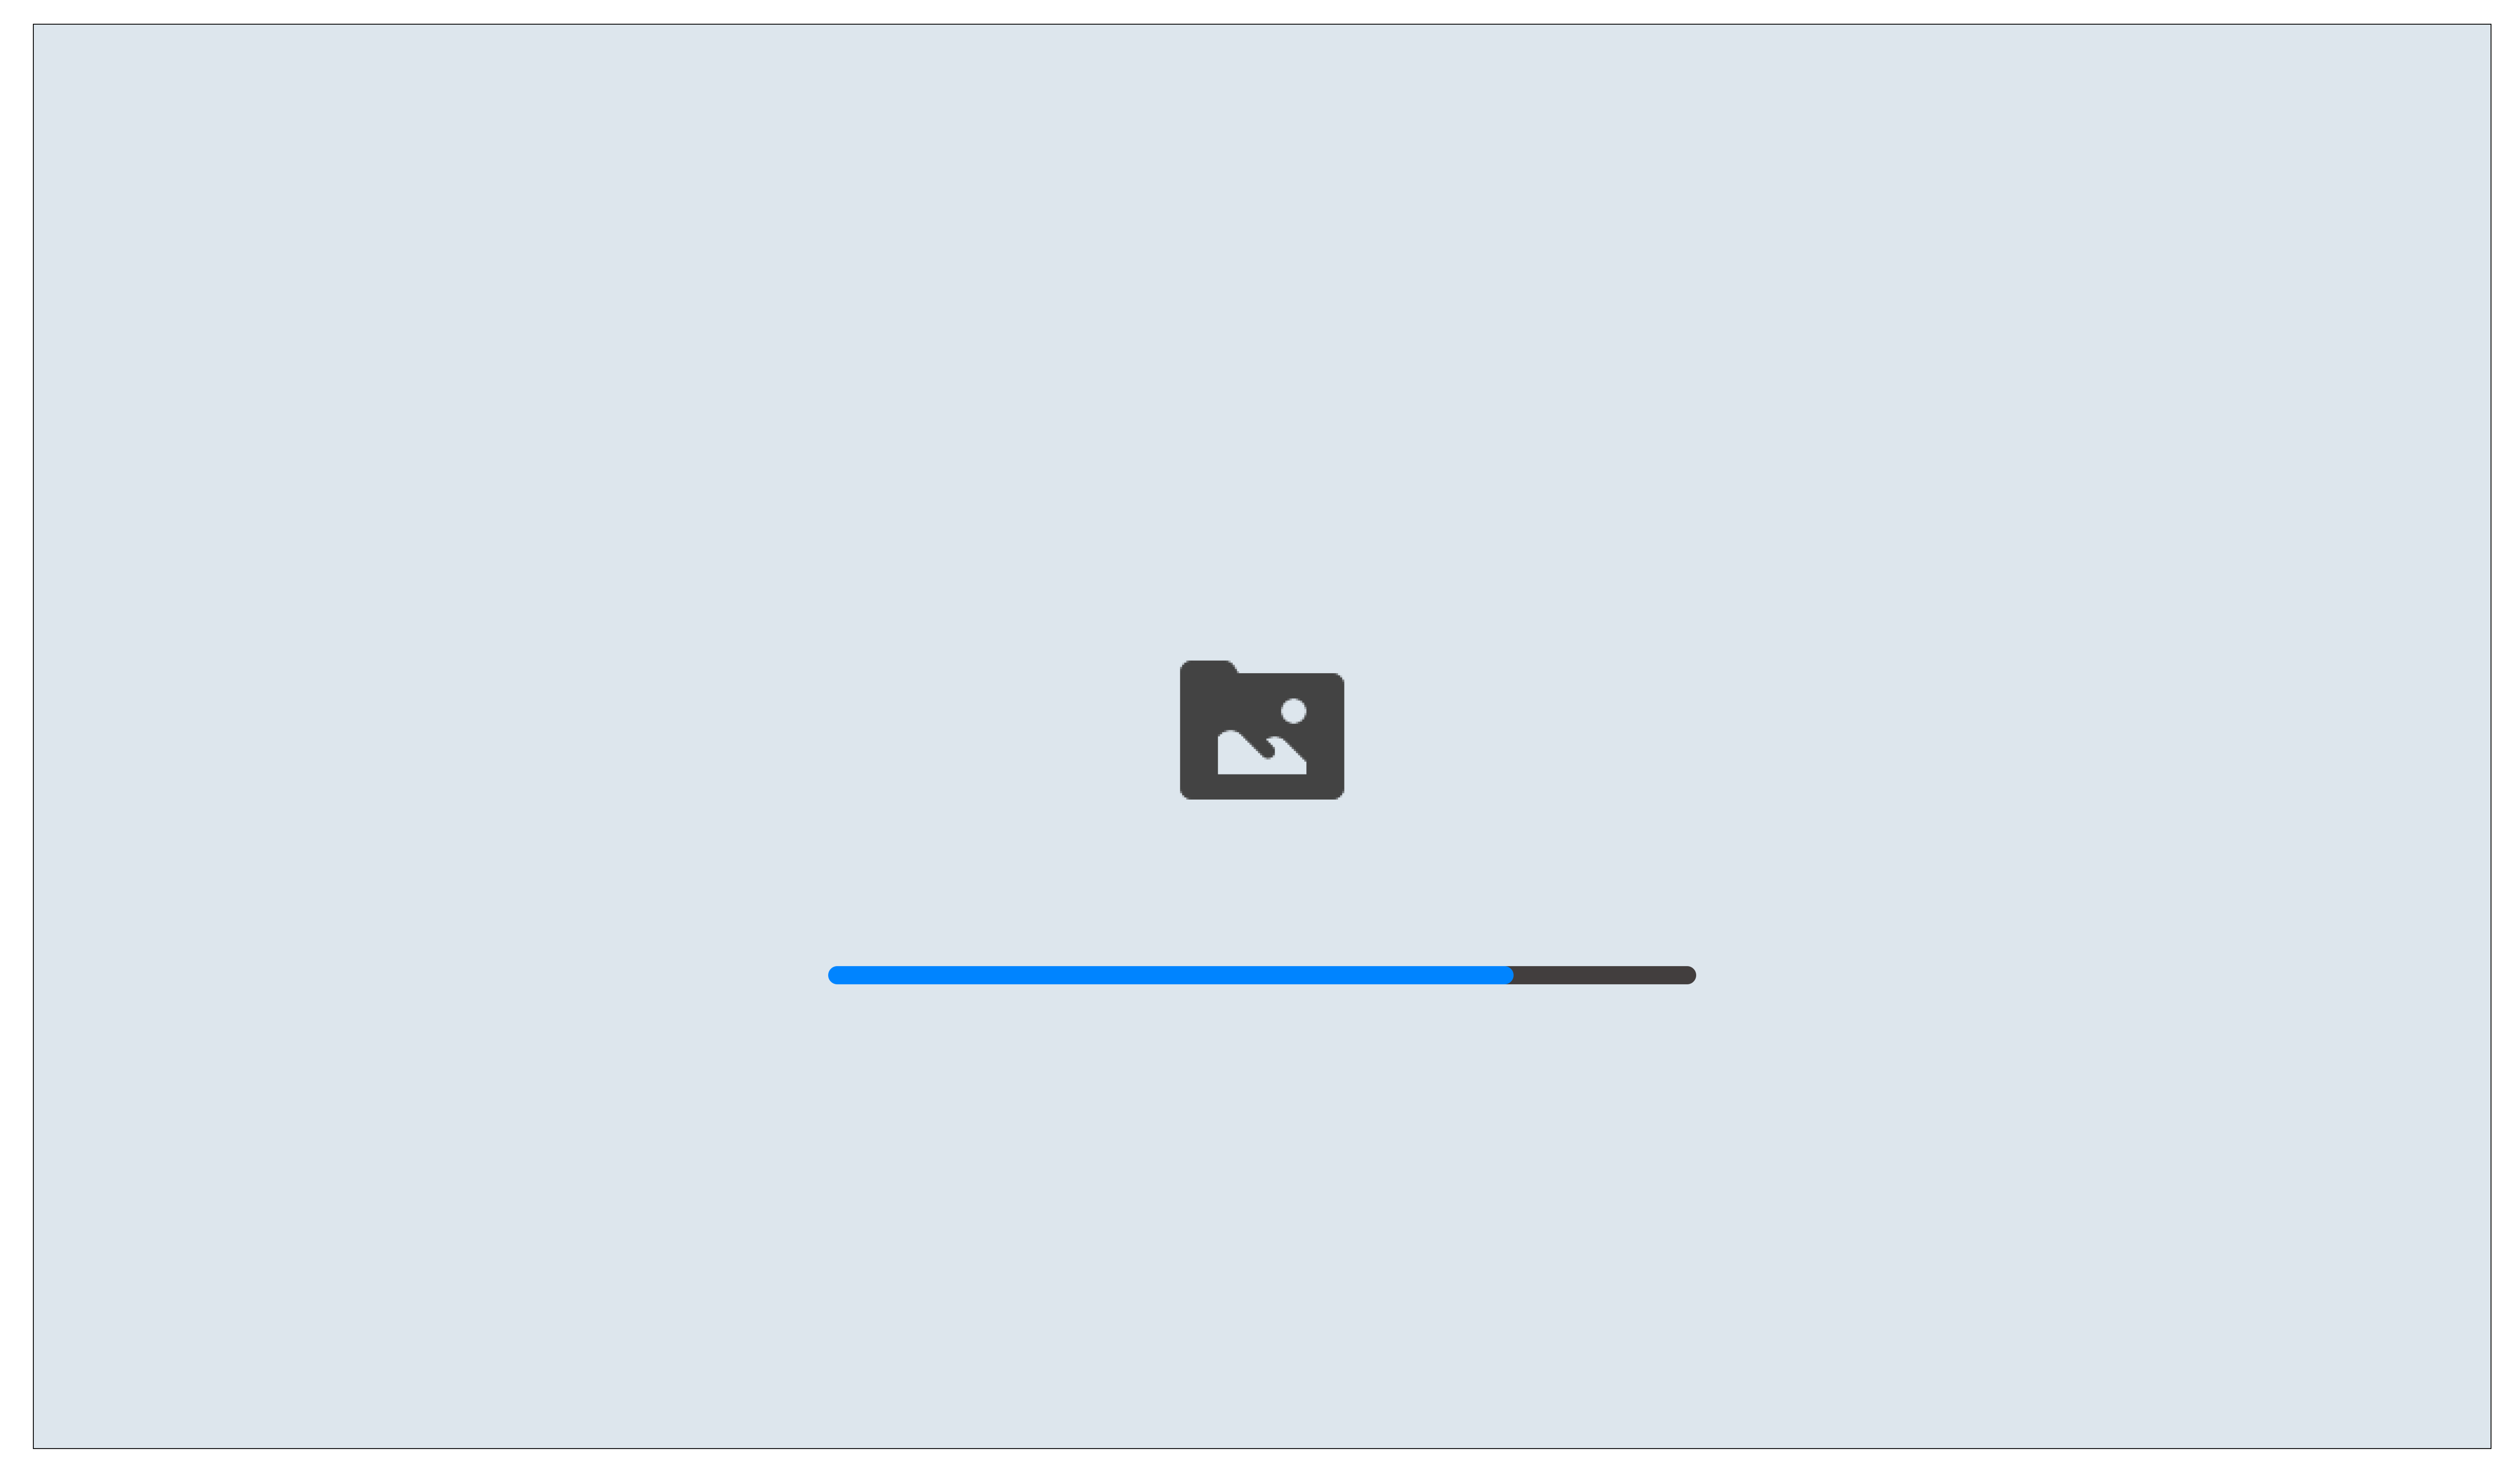
\includegraphics[width=1\textwidth, height=6cm]{chap2.images/splash web.png}
    \caption{Ecran de chargement - Web}
  \end{minipage}
  \hfill
  \begin{minipage}[t]{0.38\textwidth}
    \centering
    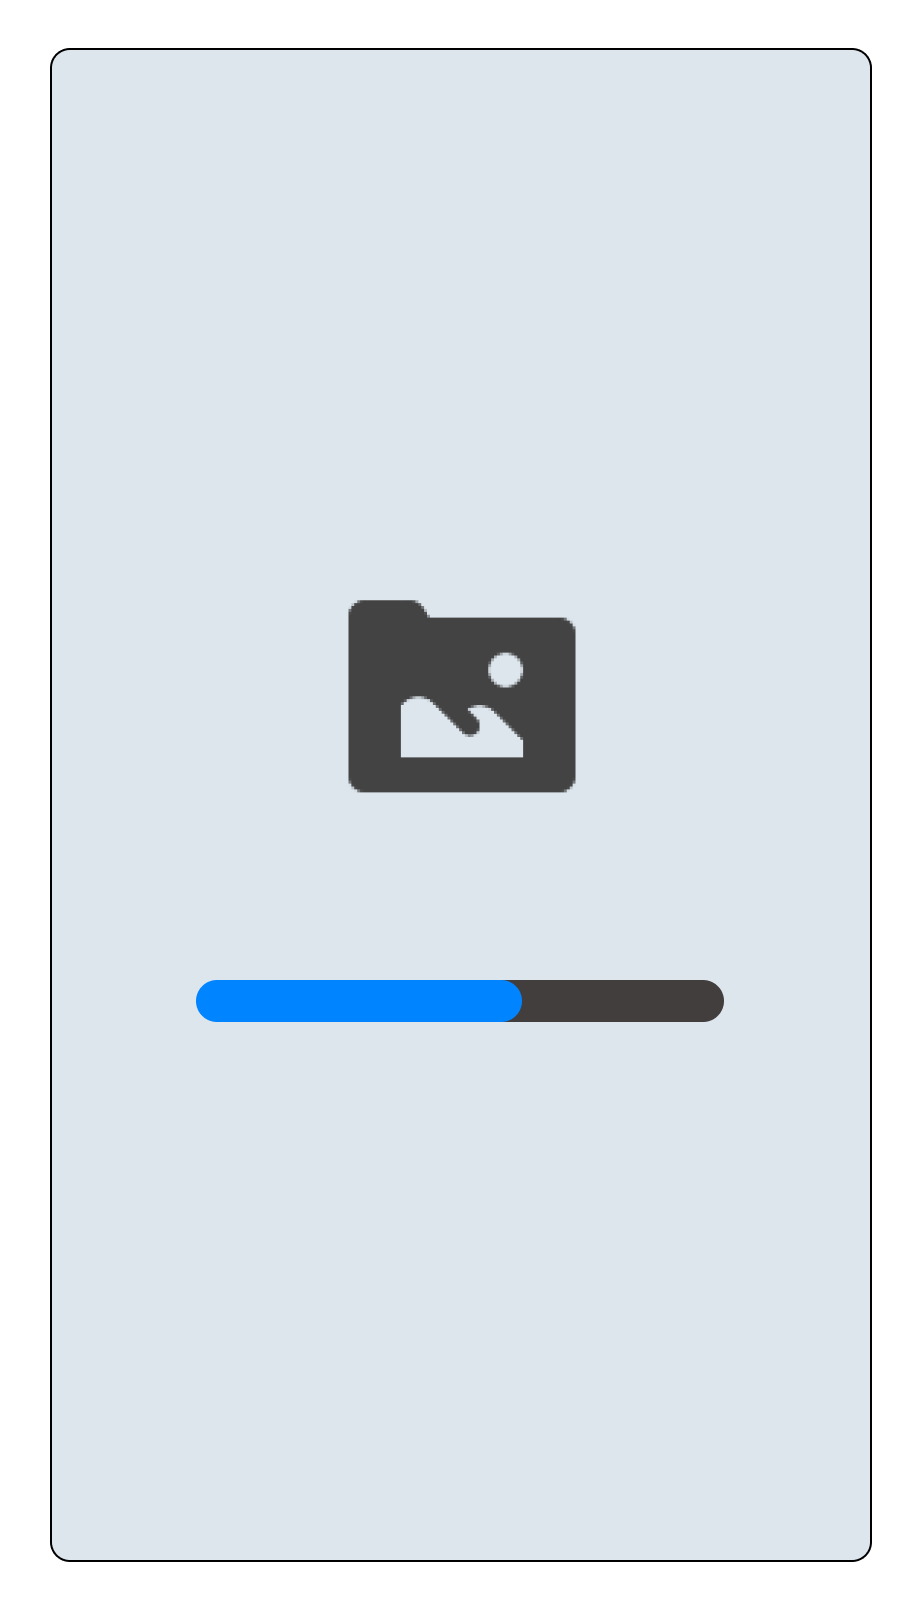
\includegraphics[width=0.6\textwidth, height=6cm]{chap2.images/splash mob.png}
    \caption{\centering{Ecran de chargement - Mobile}}
  \end{minipage}
\end{figure}


\newpage
Les figure 2.5 et 2.6 illustrent les  pages permettant a l'utilisateur de s'authentifier dans l'application.

\begin{figure}[h!]
  \centering
  \begin{minipage}[t]{0.60\textwidth}
    \centering
    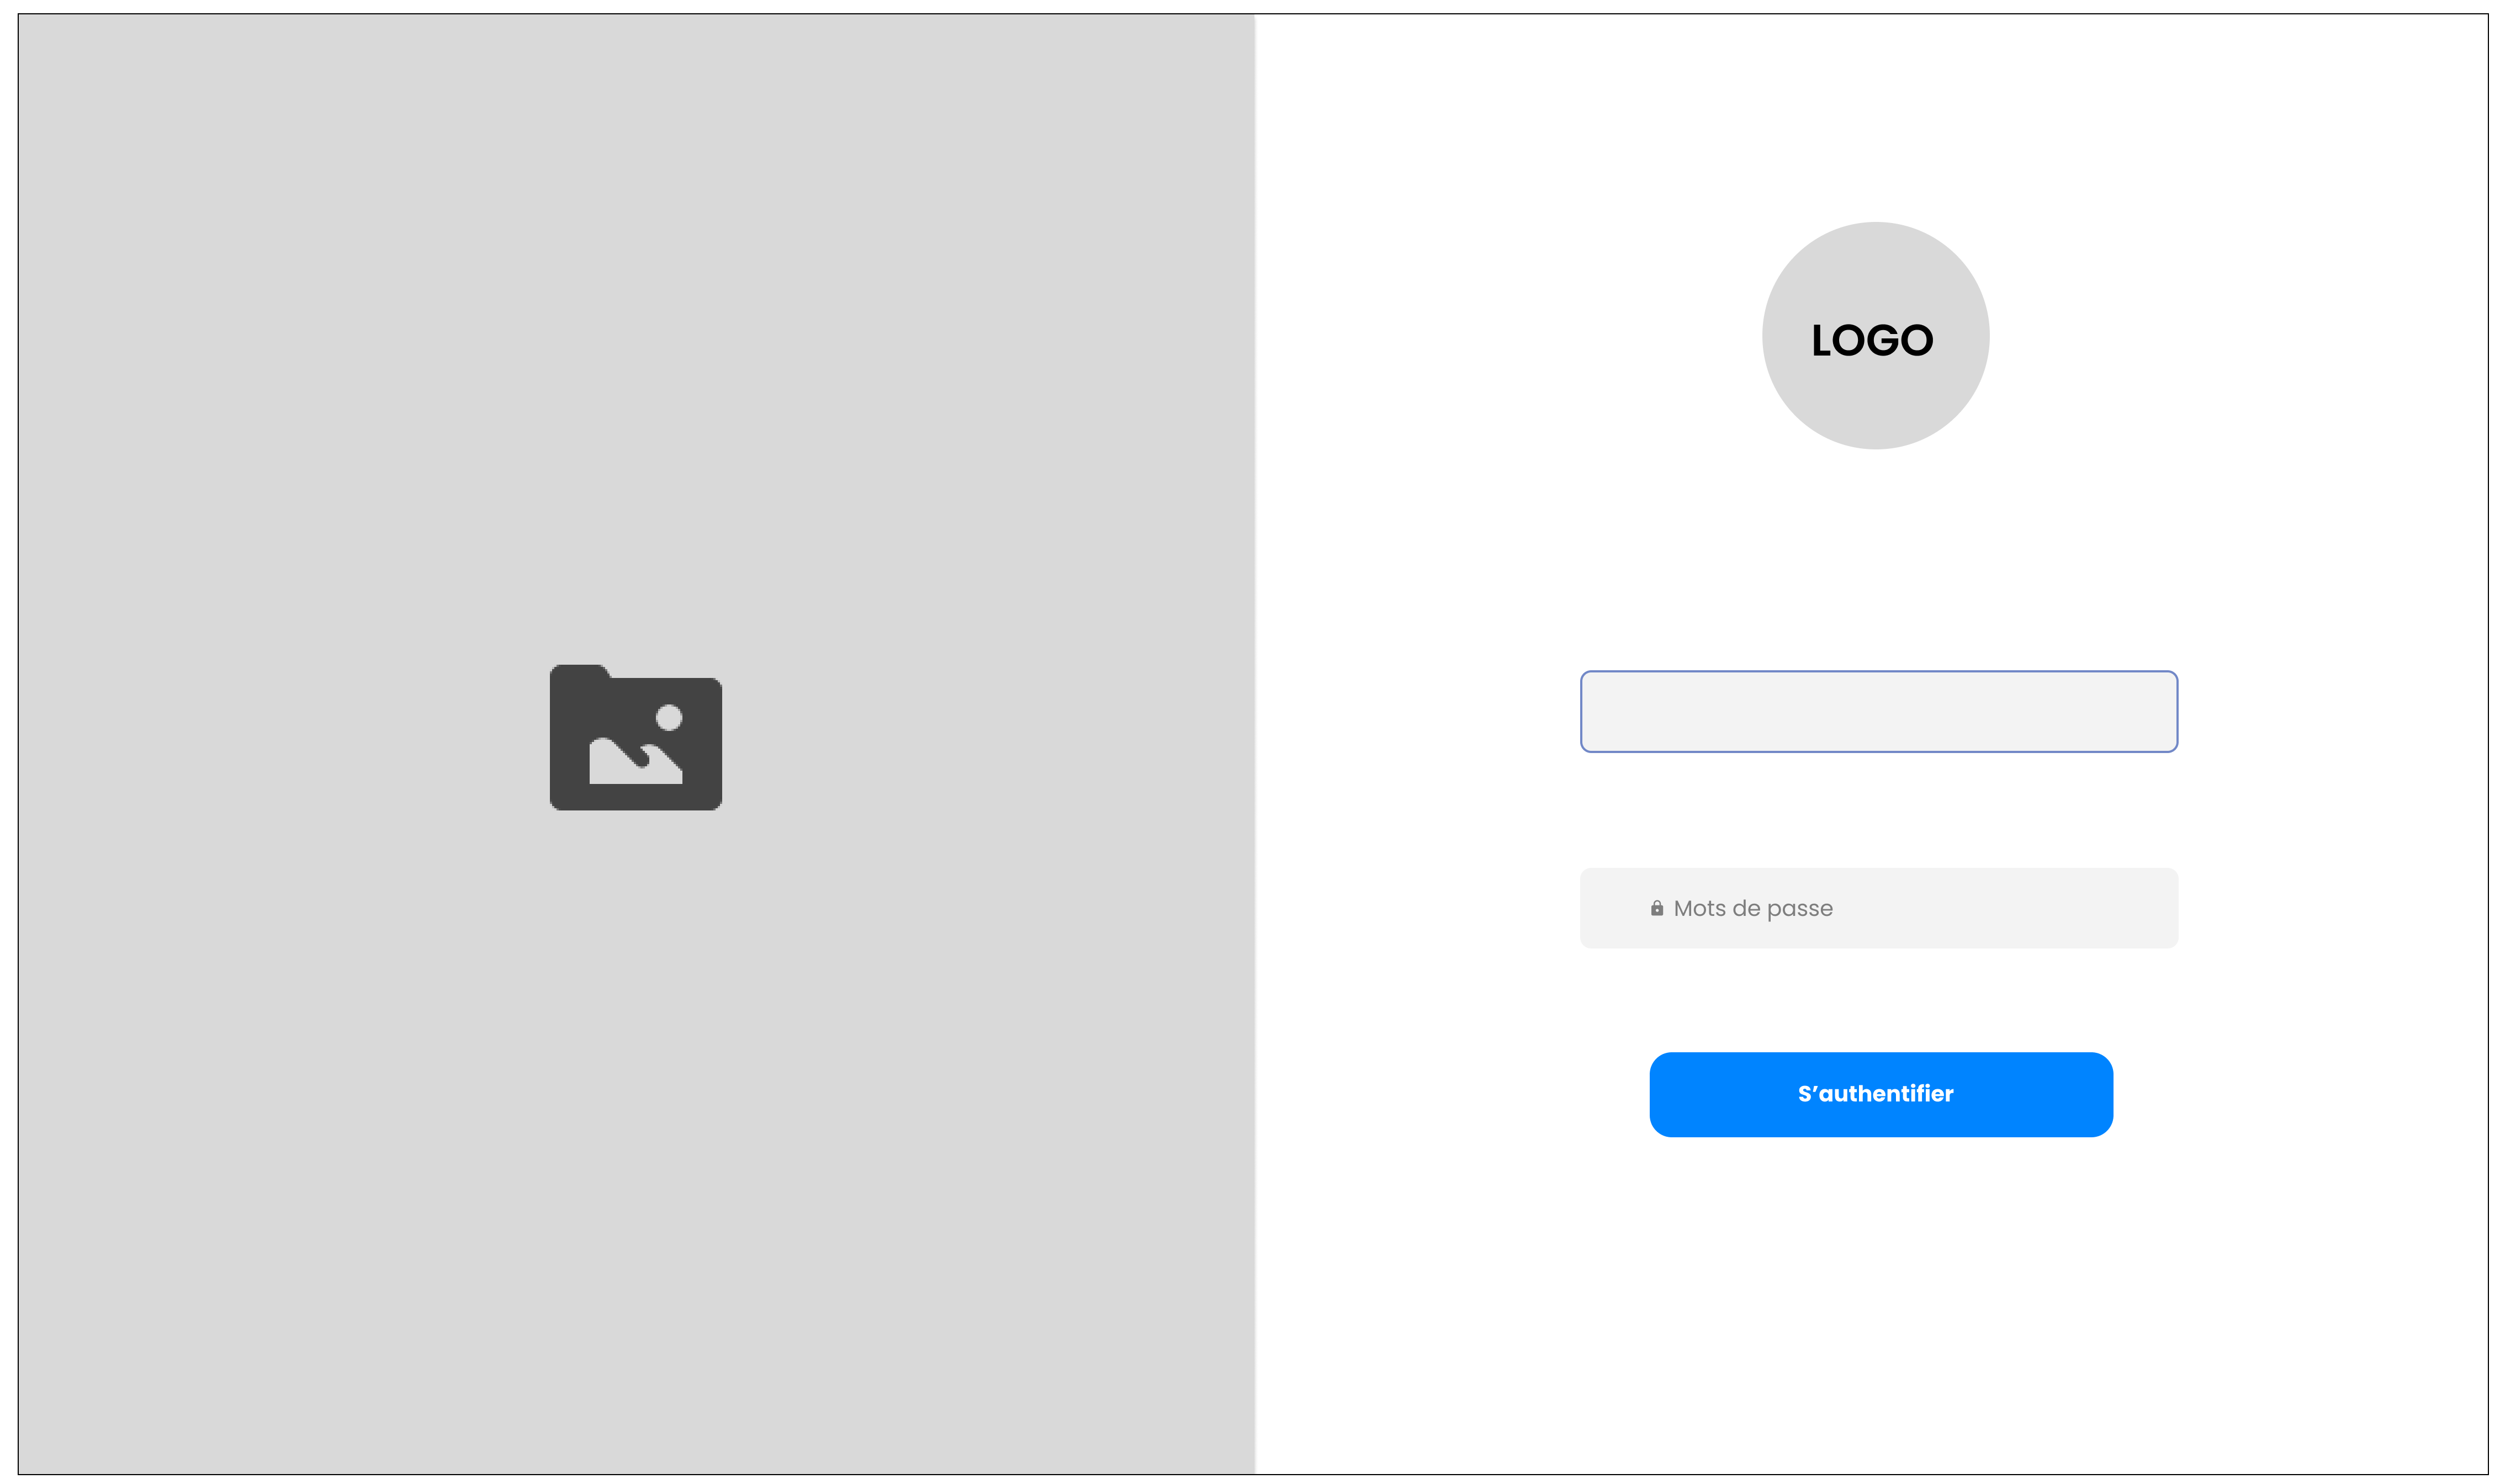
\includegraphics[width=1\textwidth, height=6cm]{chap2.images/prot authentification.png}
    \caption{Interface d'authentification - Web}
  \end{minipage}
  \hfill
  \begin{minipage}[t]{0.38\textwidth}
    \centering
    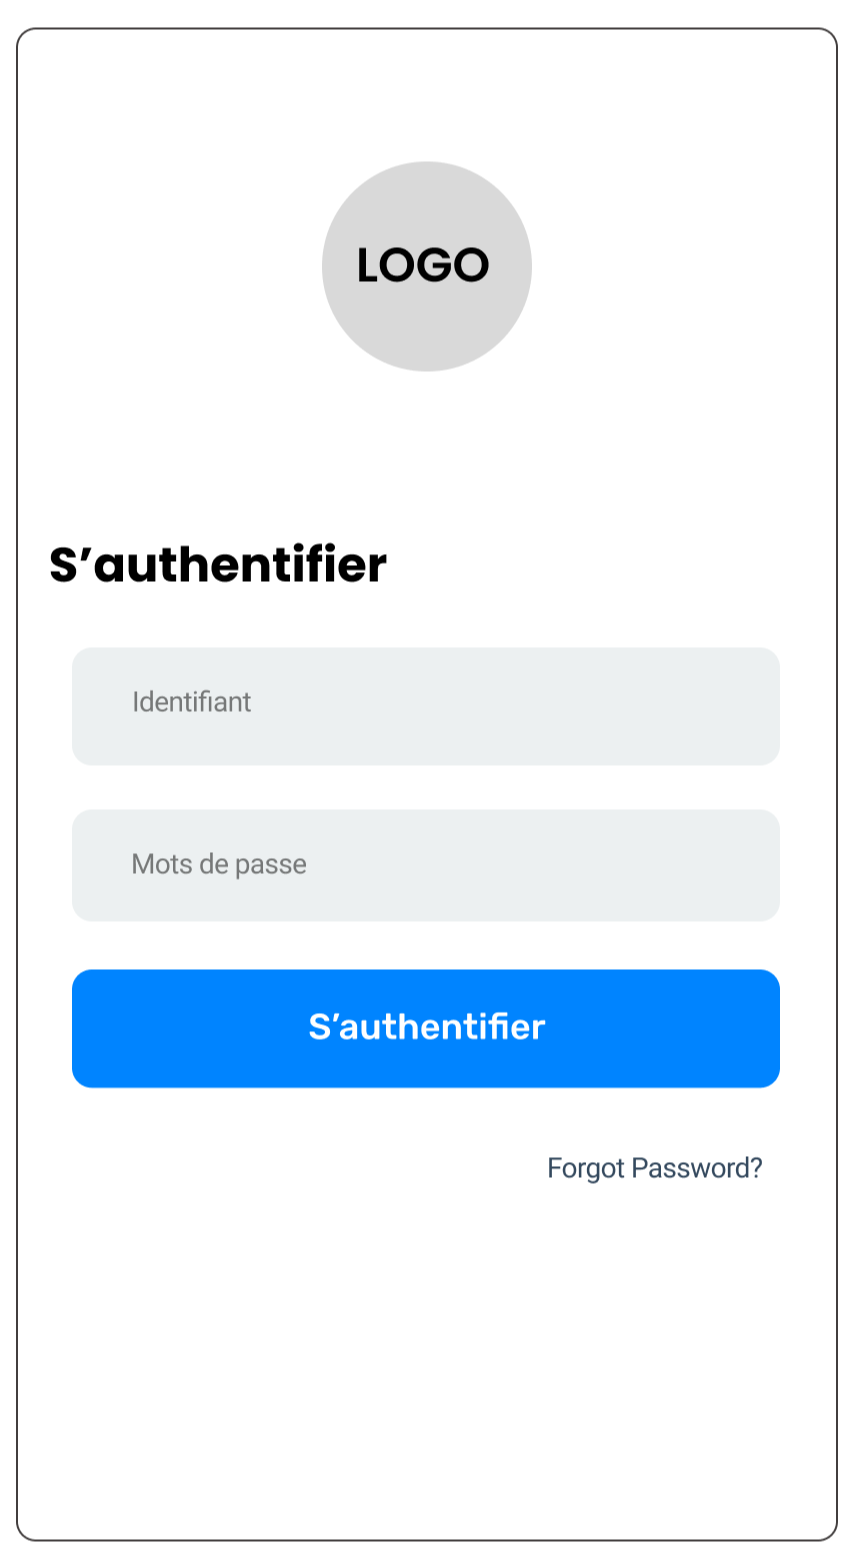
\includegraphics[width=0.6\textwidth, height=6cm]{chap2.images/prot authentification mob.png}
    \caption{\centering{Interface d'authentification - Mobile}}
  \end{minipage}
\end{figure}

\vspace{1.2cm}

Les figure 2.7 et 2.8 illustrent les  pages permettant a l'utilisateur de modifier leur profils.

\begin{figure}[h!]
  \centering
  \begin{minipage}[t]{0.60\textwidth}
    \centering
    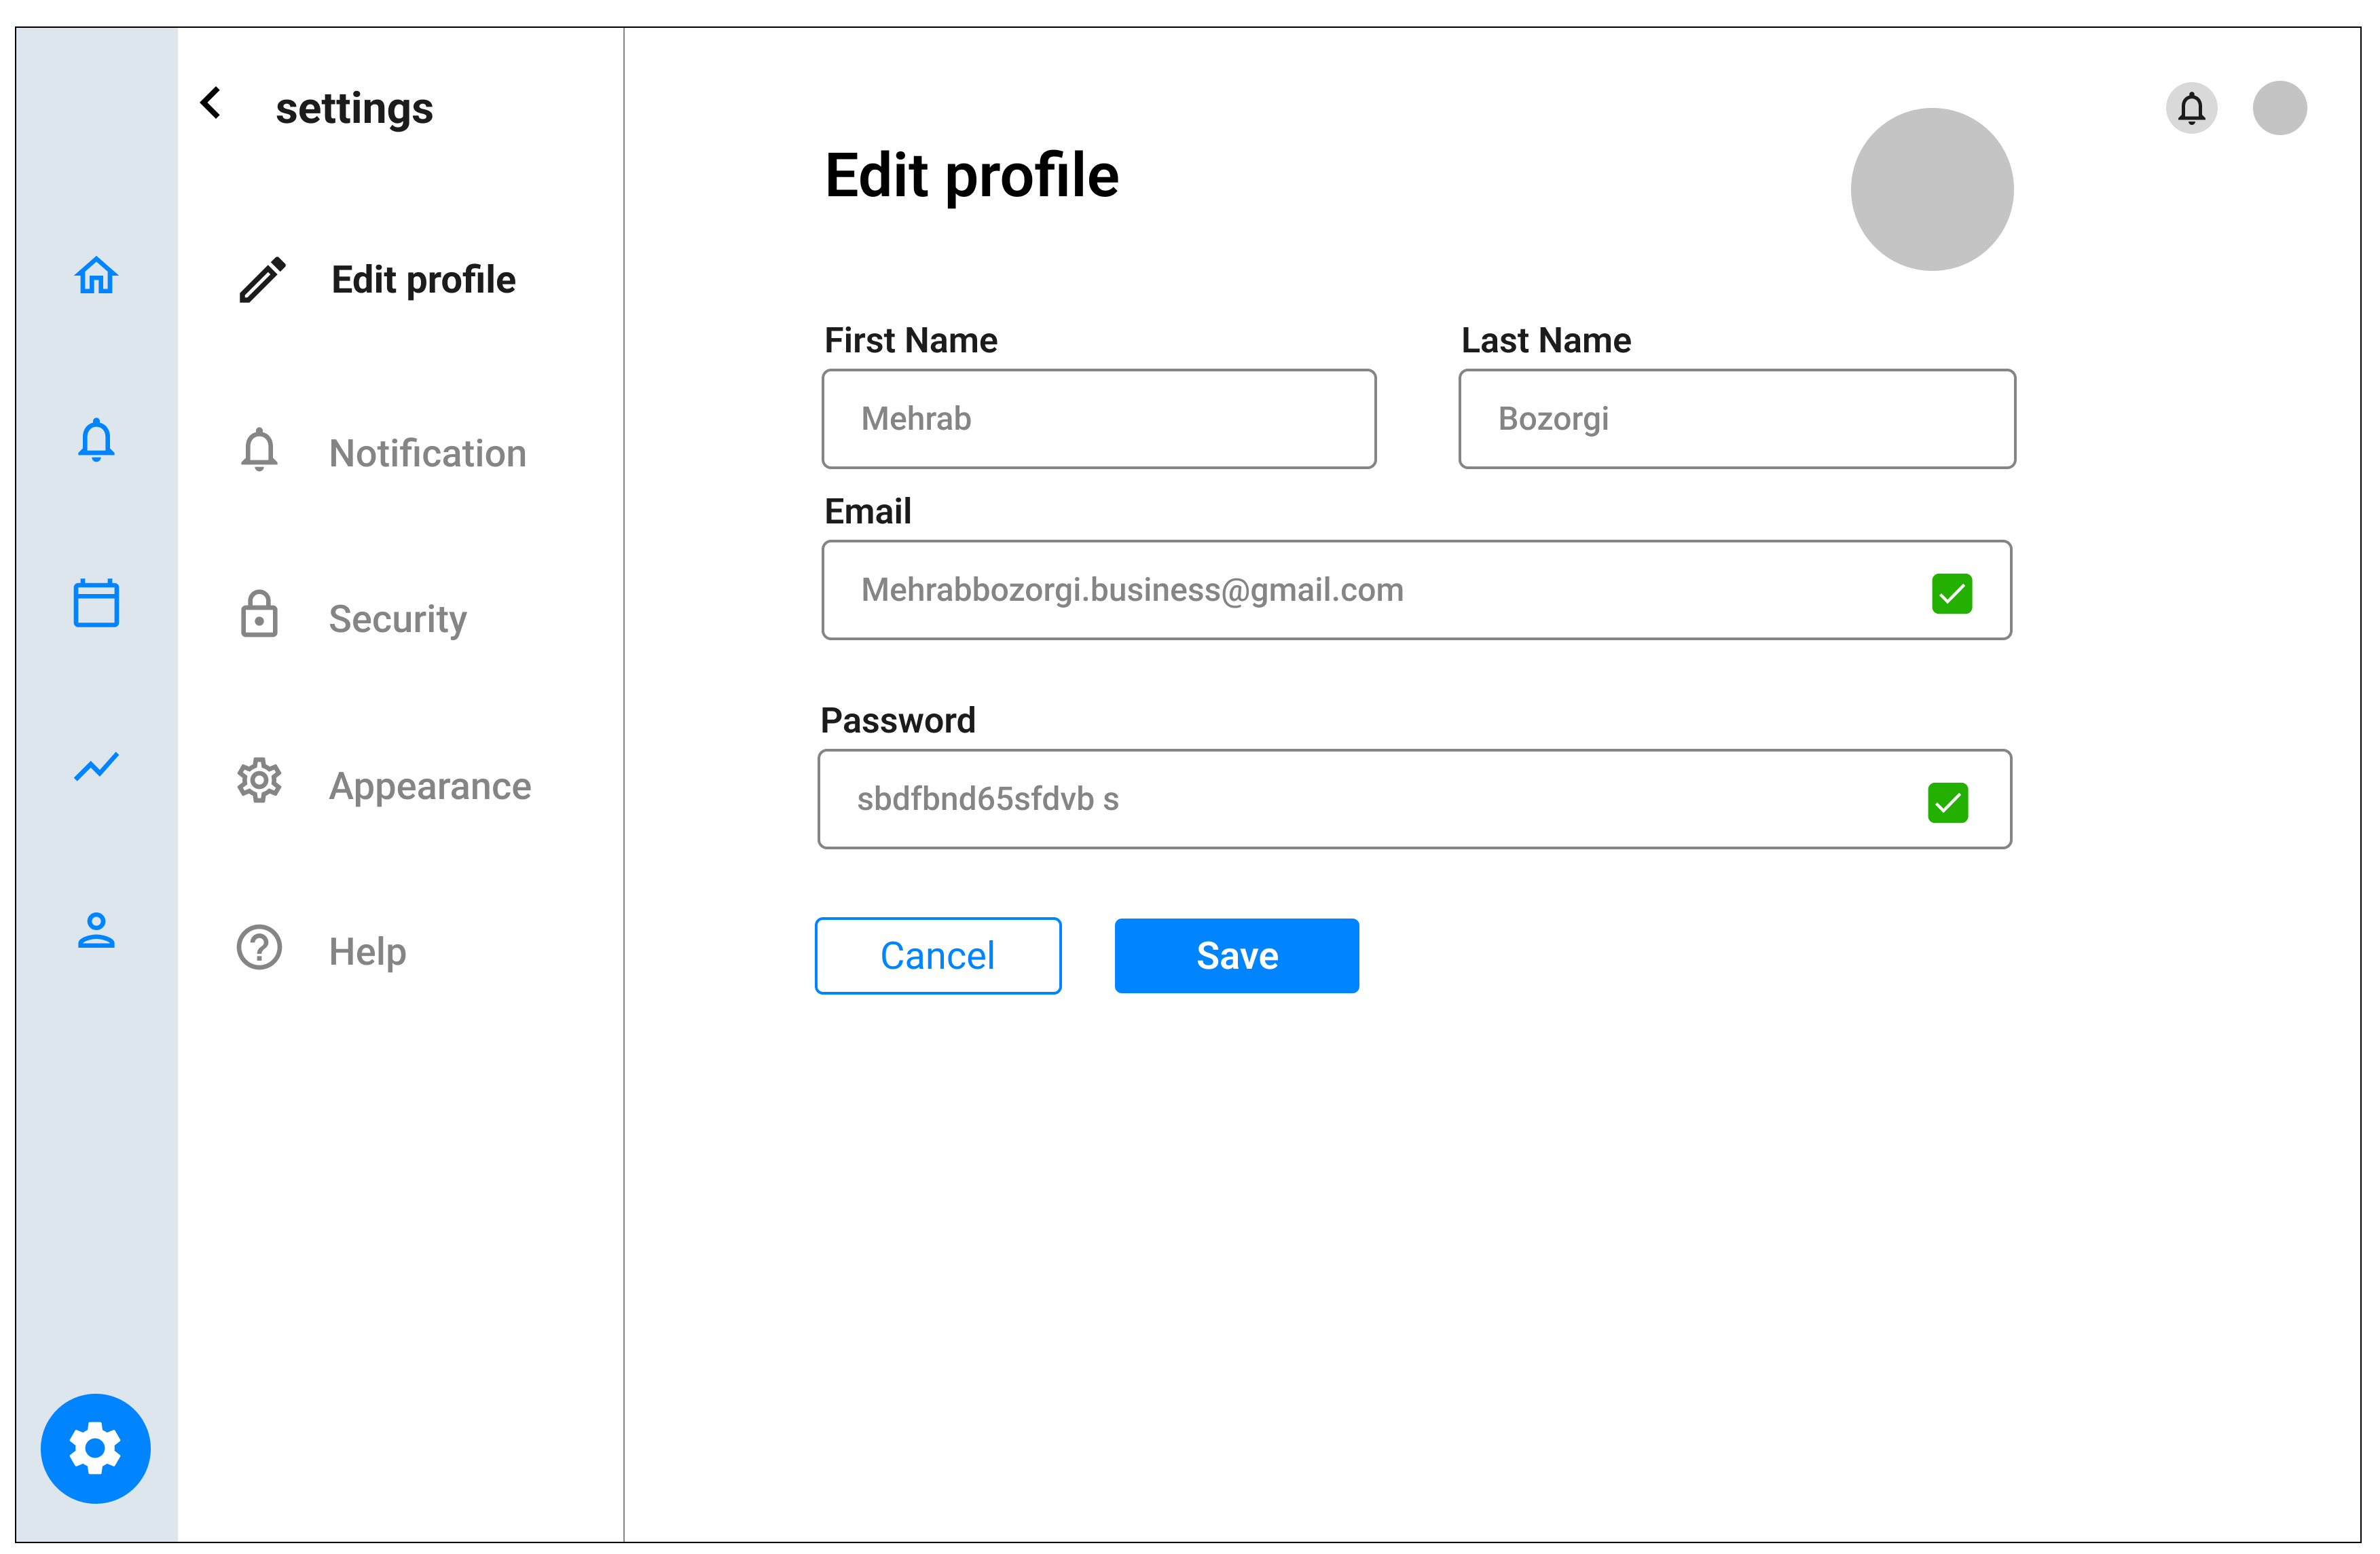
\includegraphics[width=1\textwidth, height=6cm]{chap2.images/prot modifer web.png}
    \caption{Interface de profil- Web}
  \end{minipage}
  \hfill
  \begin{minipage}[t]{0.38\textwidth}
    \centering
    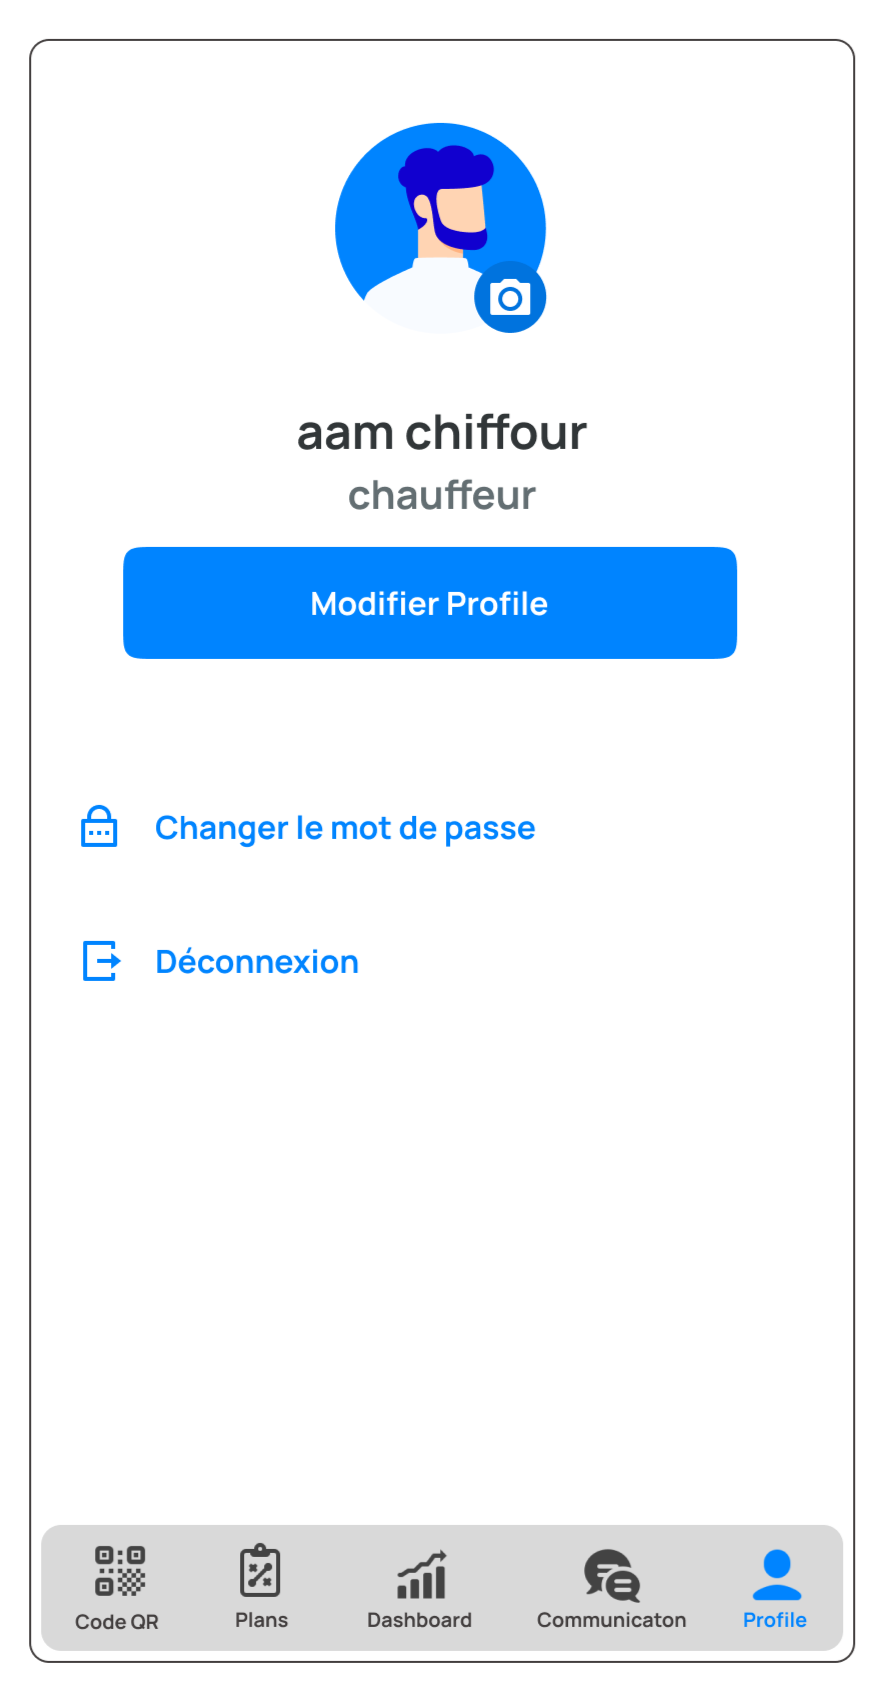
\includegraphics[width=0.6\textwidth, height=6cm]{chap2.images/prot modifier mob.png}
    \caption{\centering{Interface de profil - Mobile}}
  \end{minipage}
\end{figure}





\newpage
En plus, les figure 2.9 et 2.10 illustrent les interfaces de gestion des utilisateurs par l'administrateur.
\begin{figure}[h!]
  \centering
  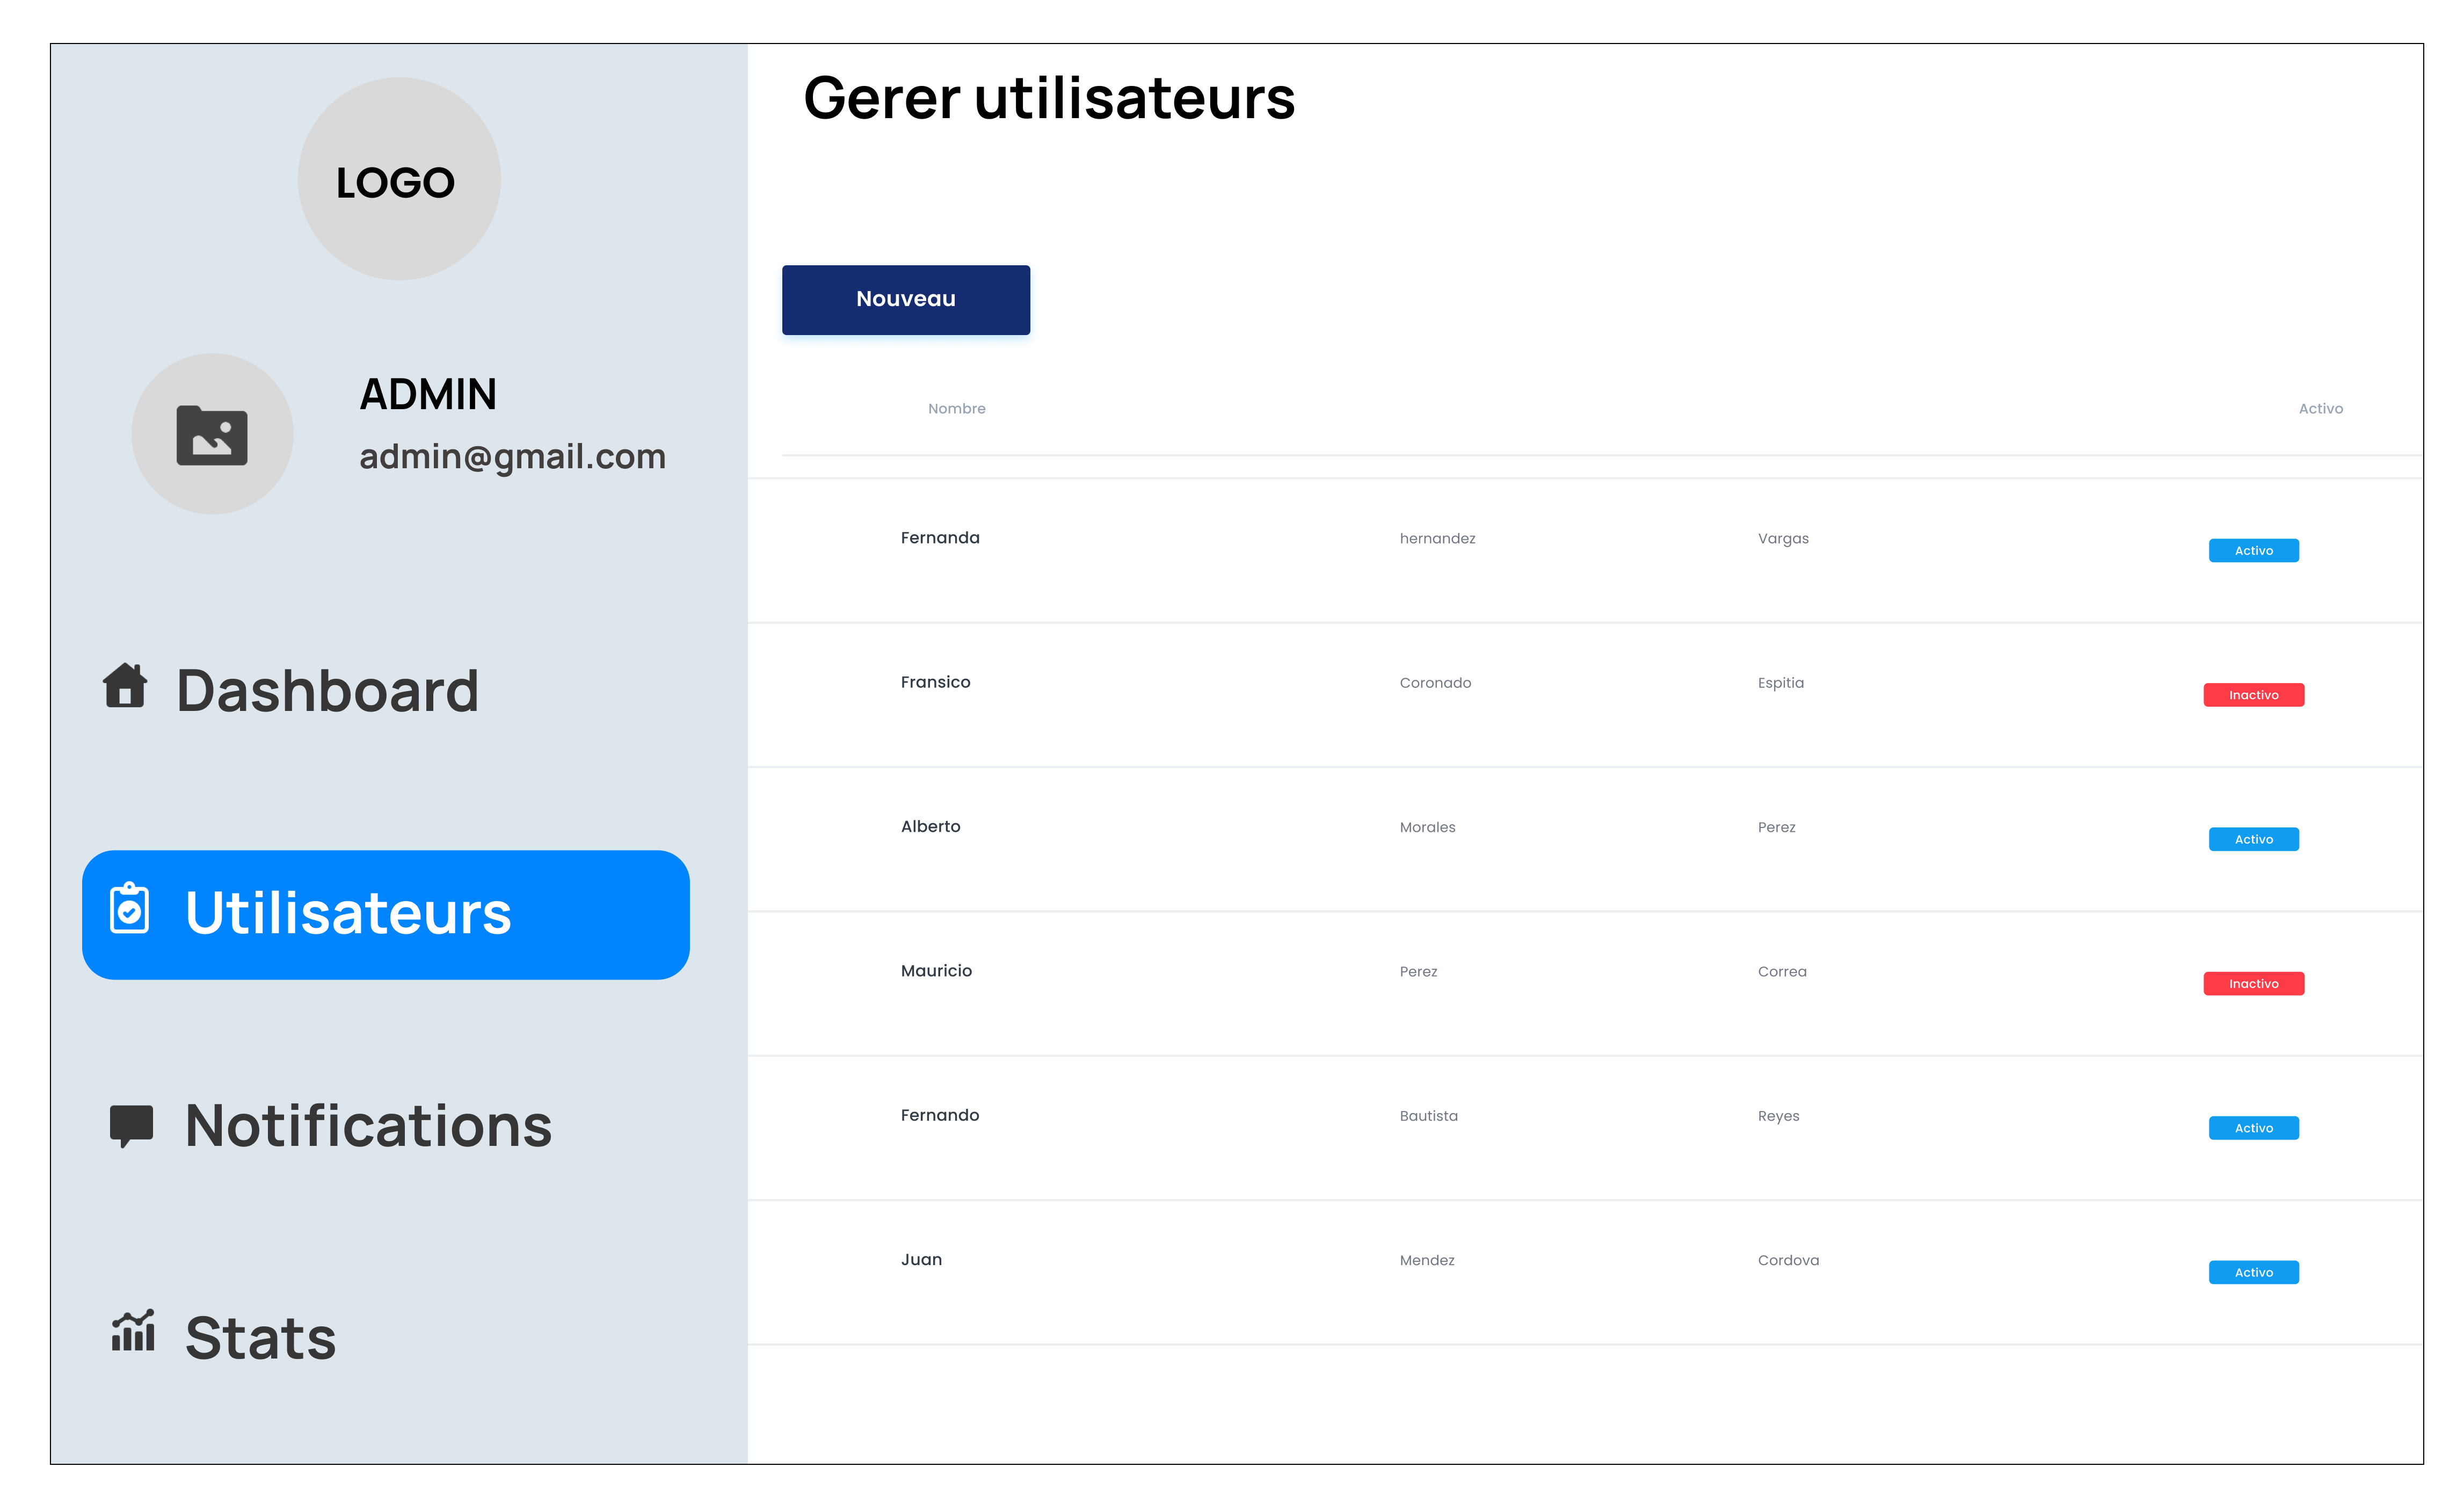
\includegraphics[width=0.9\textwidth, height=8cm]{chap2.images/prot gestion user.png}
  \caption{Interface de gestion des utilisateurs}
\end{figure}
\begin{figure}[h!]
  \centering
  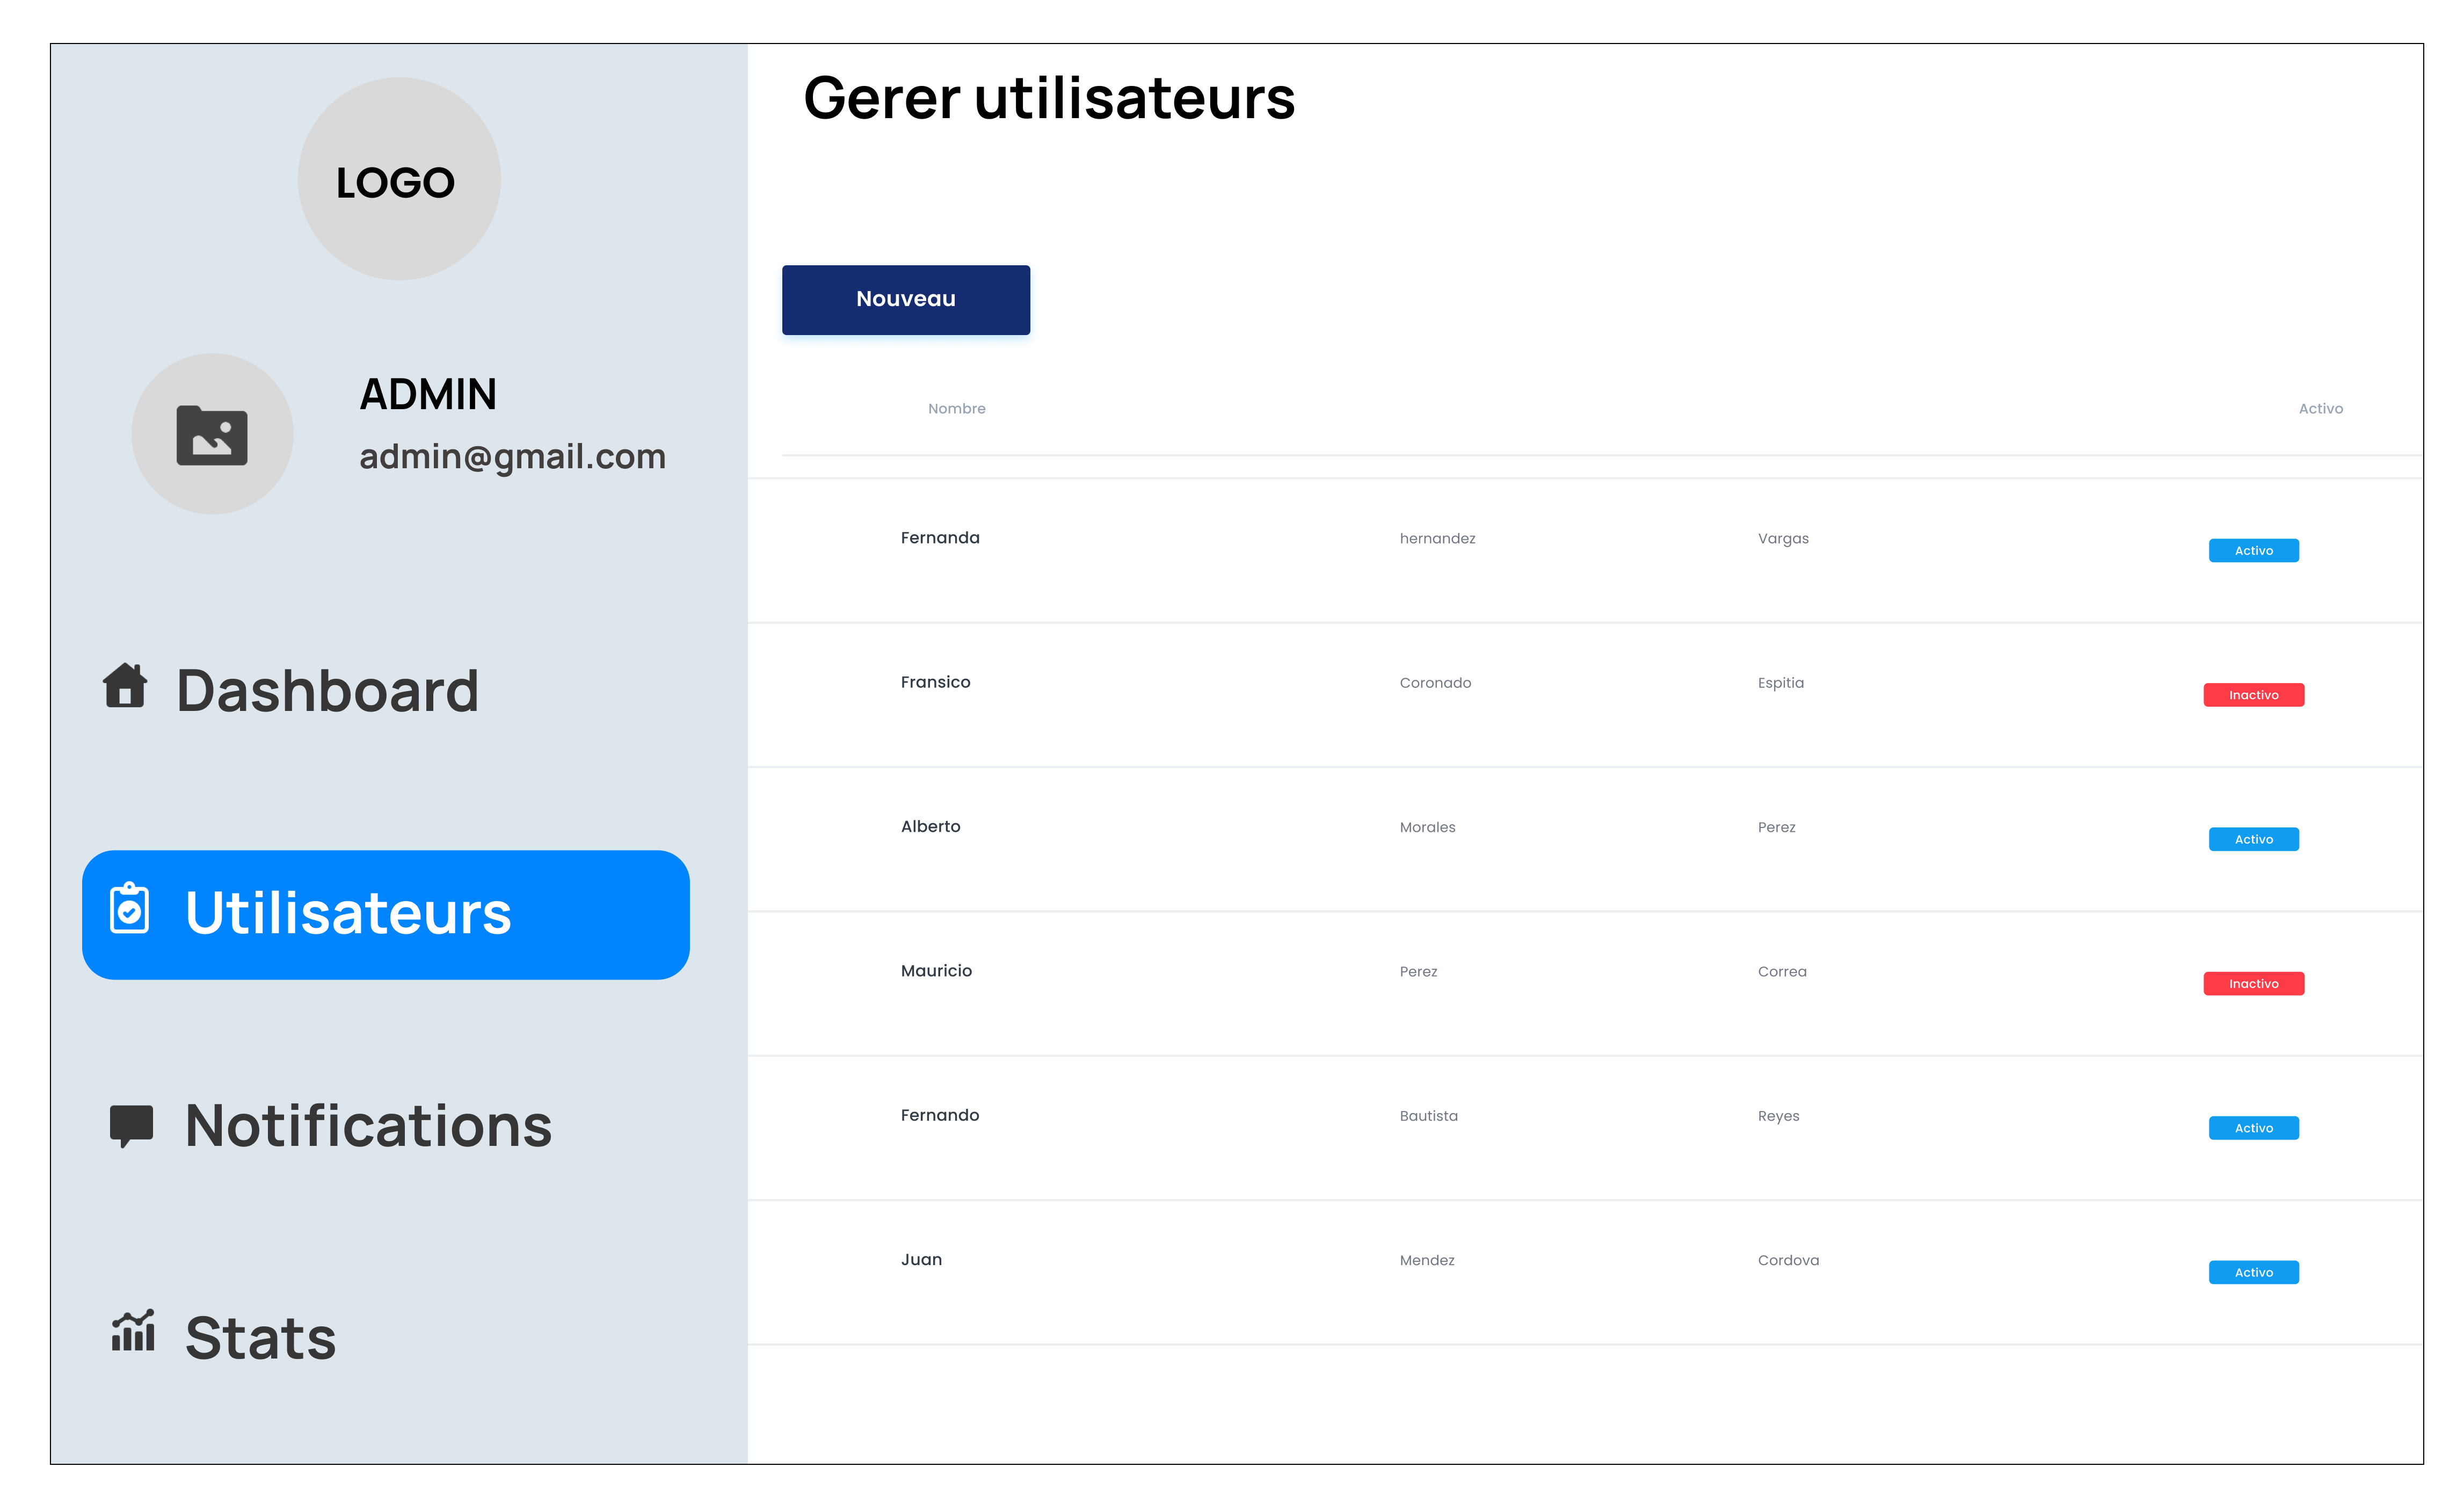
\includegraphics[width=0.9\textwidth, height=8cm]{chap2.images/prot gestion user.png}
  \caption{Interface de création d'un nouvel utilisateur}
\end{figure}

\newpage
Les figure 2.11 et 2.12 illustrent les  pages permettant ....

\begin{figure}[h!]
  \centering
  \begin{minipage}[t]{0.60\textwidth}
    \centering
    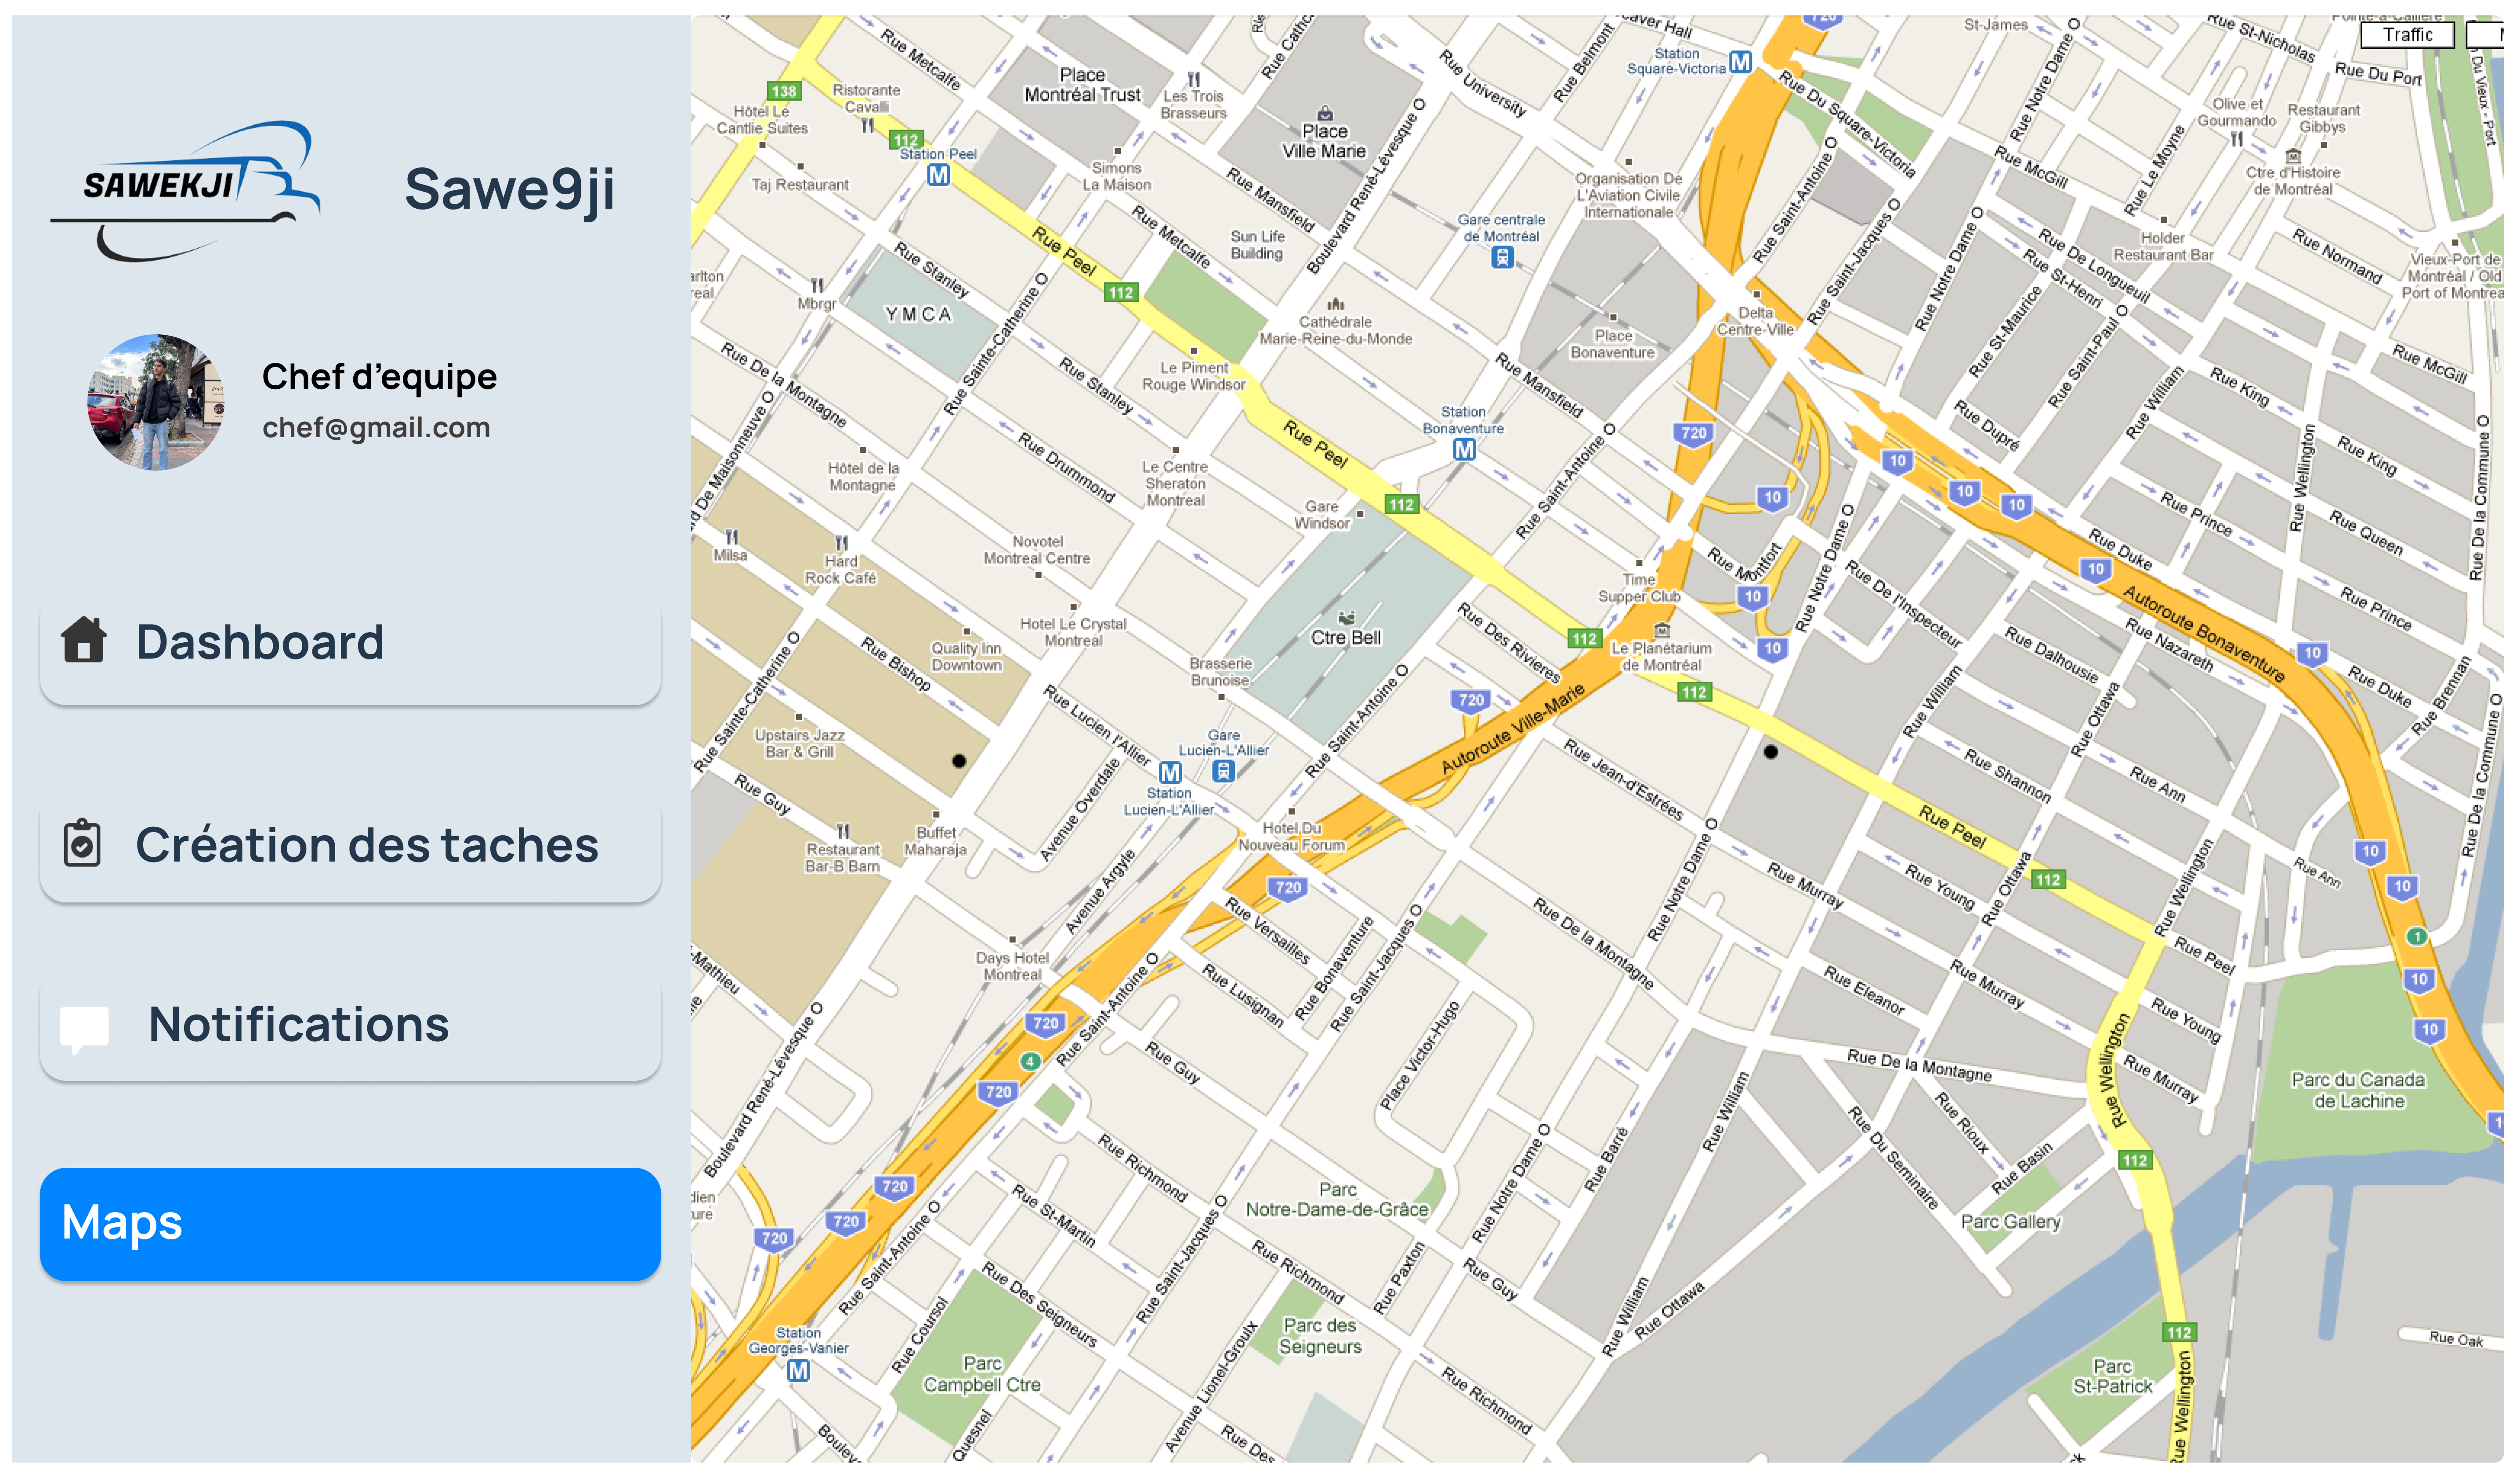
\includegraphics[width=1\textwidth, height=6cm]{chap2.images/maps web.png}
    \caption{map- Web}
  \end{minipage}
  \hfill
  \begin{minipage}[t]{0.38\textwidth}
    \centering
    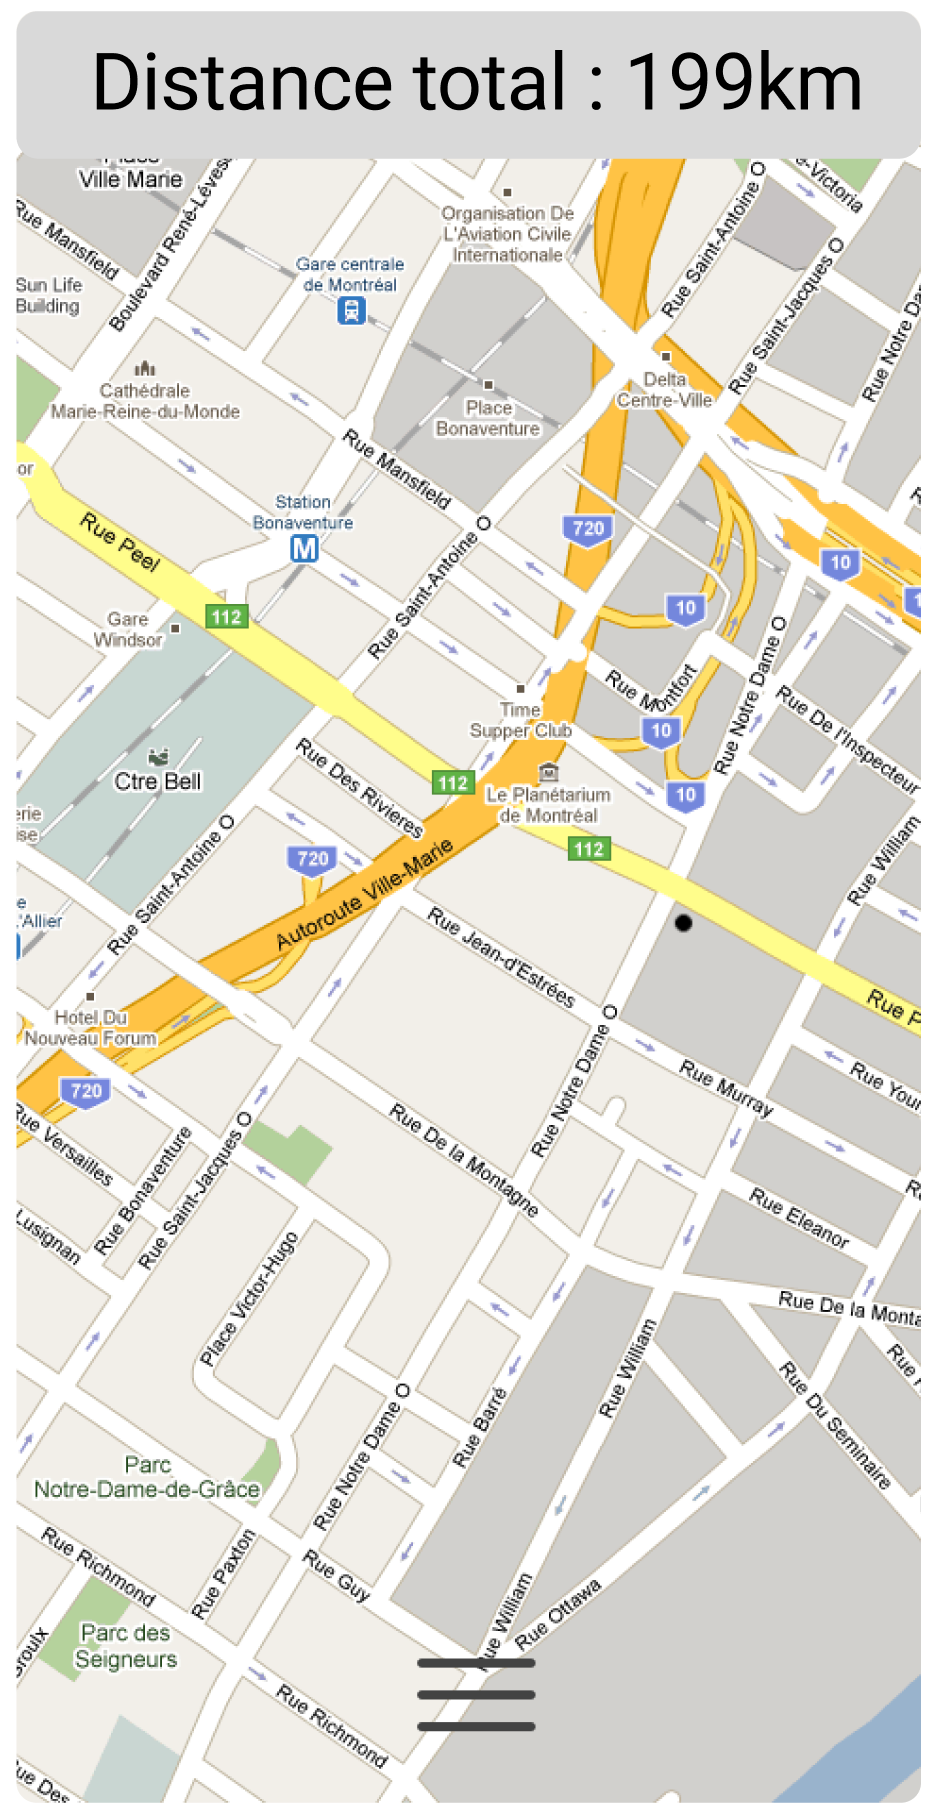
\includegraphics[width=0.6\textwidth, height=6cm]{chap2.images/map mobile.png}
    \caption{\centering{map - Mobile}}
  \end{minipage}
\end{figure}


%__________________________________________________________________________________________________________

\newpage
\subsection{Charte Graphique}

La phase de création de la charte graphique a été précédée par une séance de brainstorming afin de choisir la palette adéquate ainsi que le nom et le logo de l’application.

\begin{figure}[h!]
  \centering
  \begin{minipage}[t]{0.45\textwidth}
    \centering
    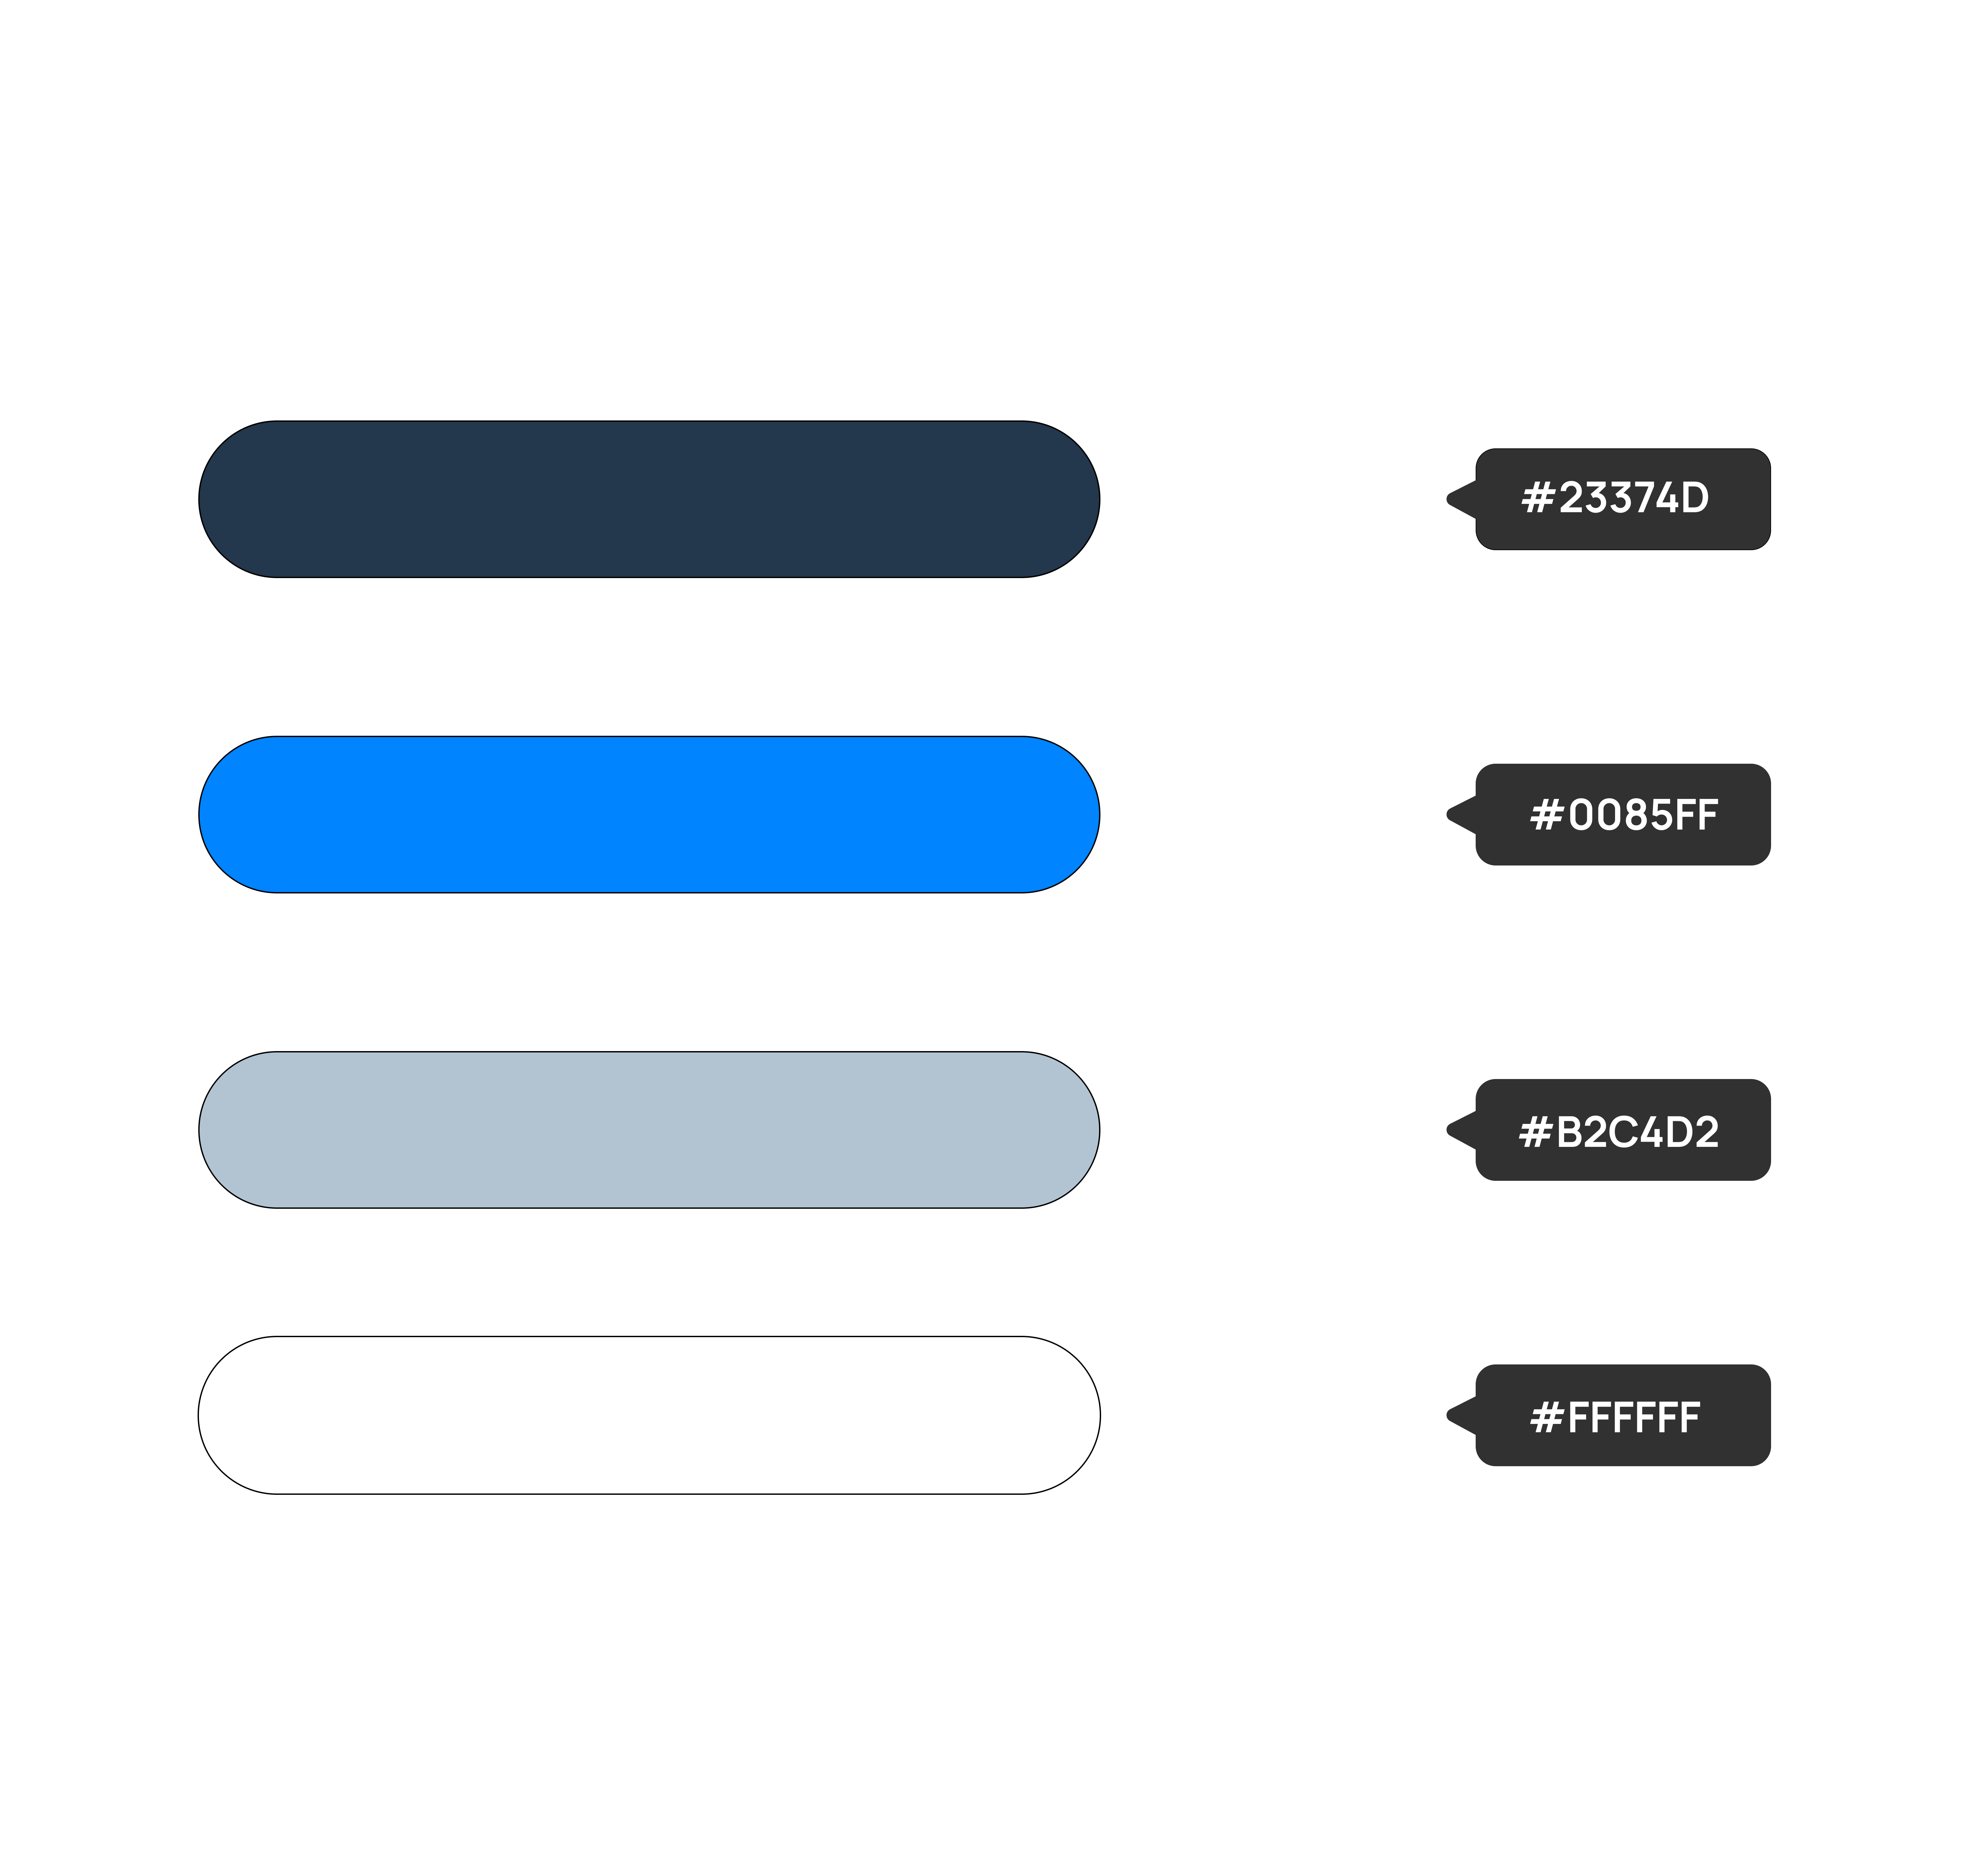
\includegraphics[width=1\textwidth]{chap2.images/palette.png}
    \caption{la palette de couleurs}
  \end{minipage}
  \hfill
  \begin{minipage}[t]{0.45\textwidth}
    \centering
    
\includegraphics[width=0.8\textwidth]{chap2.images/logo.png}
    \caption{\centering{logo}}
  \end{minipage}
\end{figure}
%__________________________________________________________________________________________________________

\subsection{Plan de l'application}
Dans cette section nous exposerons, dans les figures 2.5, 2.6, 2.7 et 2.8 l'organigramme des interfaces de l'application de nos profils d'acteurs à savoir: L'administrateur de l'application, le chauffeur, le mécanicien  et le chef d'equipe .\\

\subsubsection{Diagramme de flux utilisateur}
Le flux utilisateur est une représentation visuelle du chemin qu'un utilisateur suit pour atteindre l’objectif d’application . Voici les éléments d'un flux utilisateur : \\

\begin{itemize}[label=$\bullet$]
  \item \textbf{Flèches d'option de transition}: Ces flèches représentent les différentes options de choix que l'utilisateur peut faire pour avancer ou reculer dans le flux utilisateur.

  \item \textbf{Page}: Cela représente une seule page avec laquelle un utilisateur interagit.

  \item \textbf{Section dans la page}: Il s'agit de zones spécifiques sur une page, telles qu'un formulaire ou un menu de navigation.

  \item \textbf{Point final}: C'est le résultat final du flux utilisateur.

  \item \textbf{Entrée d'informations}: Ce sont les entrées requises de l'utilisateur, telles que remplir un formulaire ou saisir des informations de connexion.

  \item \textbf{Décision}: Ils représentent un choix ou une décision que l'utilisateur doit prendre.

  \item \textbf{Traitement des données}: Cela représente tout traitement de données qui se produit pendant le flux utilisateur.
\end{itemize}

\bigskip
\textbf{Flux utilisateur ( Définition des éléments ):}
\begin{figure}[htbp]
  \centering
  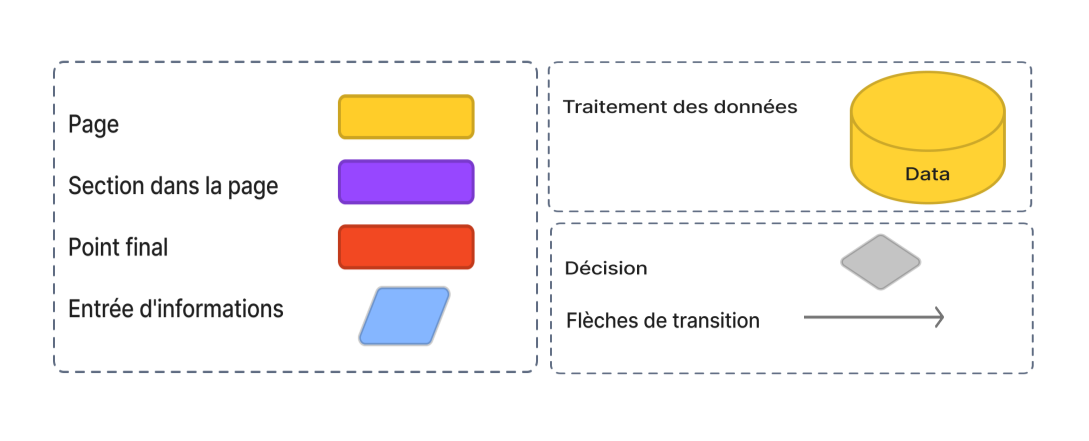
\includegraphics[width=0.9\textwidth]{chap2.images/user flow ( Définition des éléments ).png}
  \caption{Flux utilisateur : Définition des éléments}
\end{figure}


\bigskip
\textbf{Vue globale sur les flux d’utilisateurs :}
\begin{figure}[htbp]
  \centering
  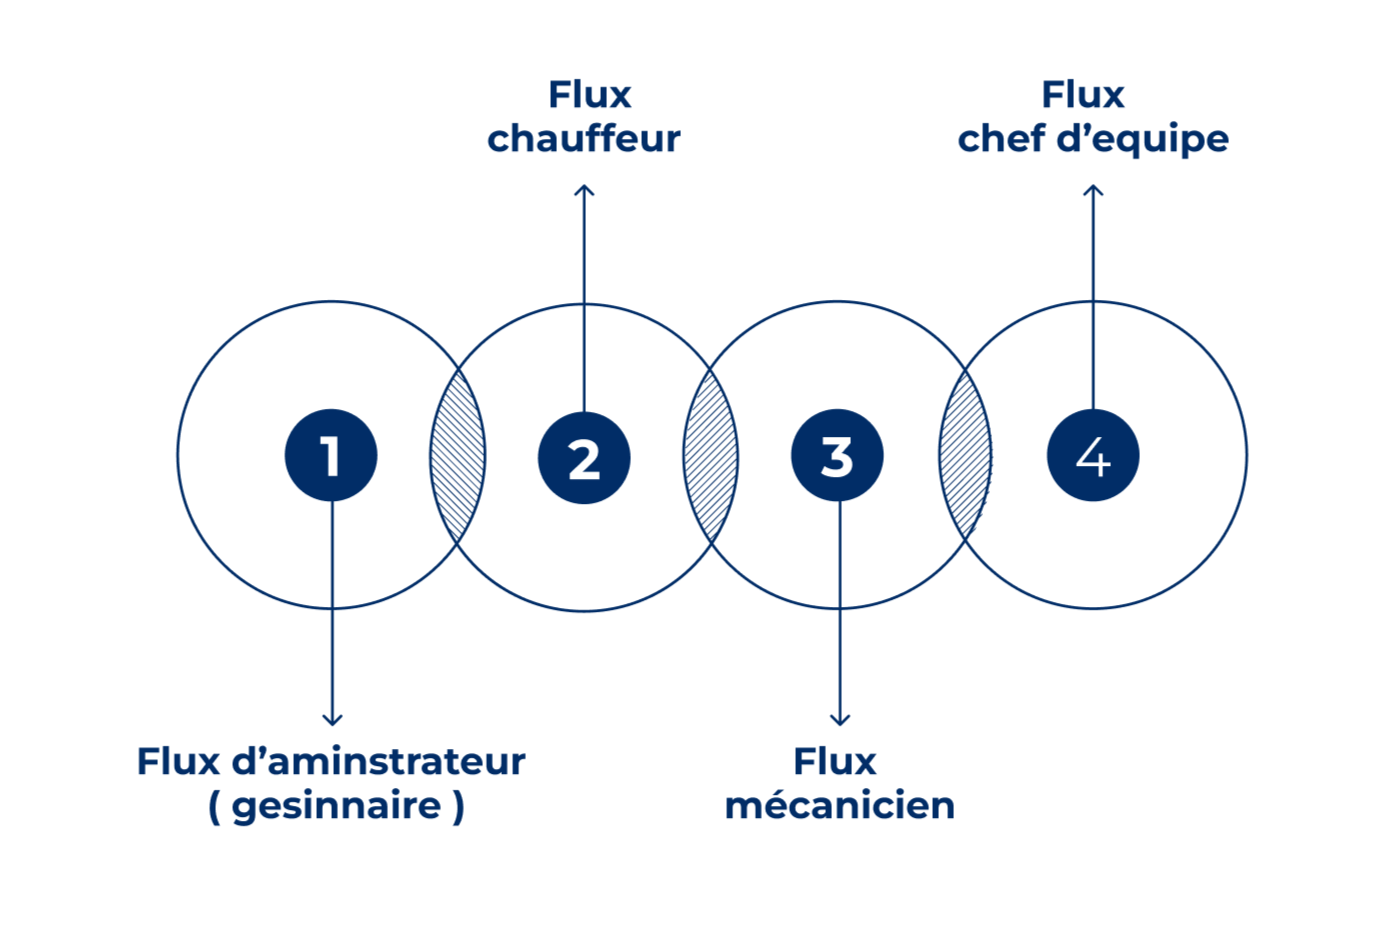
\includegraphics[width=0.7\textwidth]{chap2.images/vue global user flow.png}
  \caption{Vue globale sur les flux d'utilisateurs}
\end{figure}




\newpage
\subsubsection{Flux administrateur}
\begin{figure}[htbp]
  \centering
  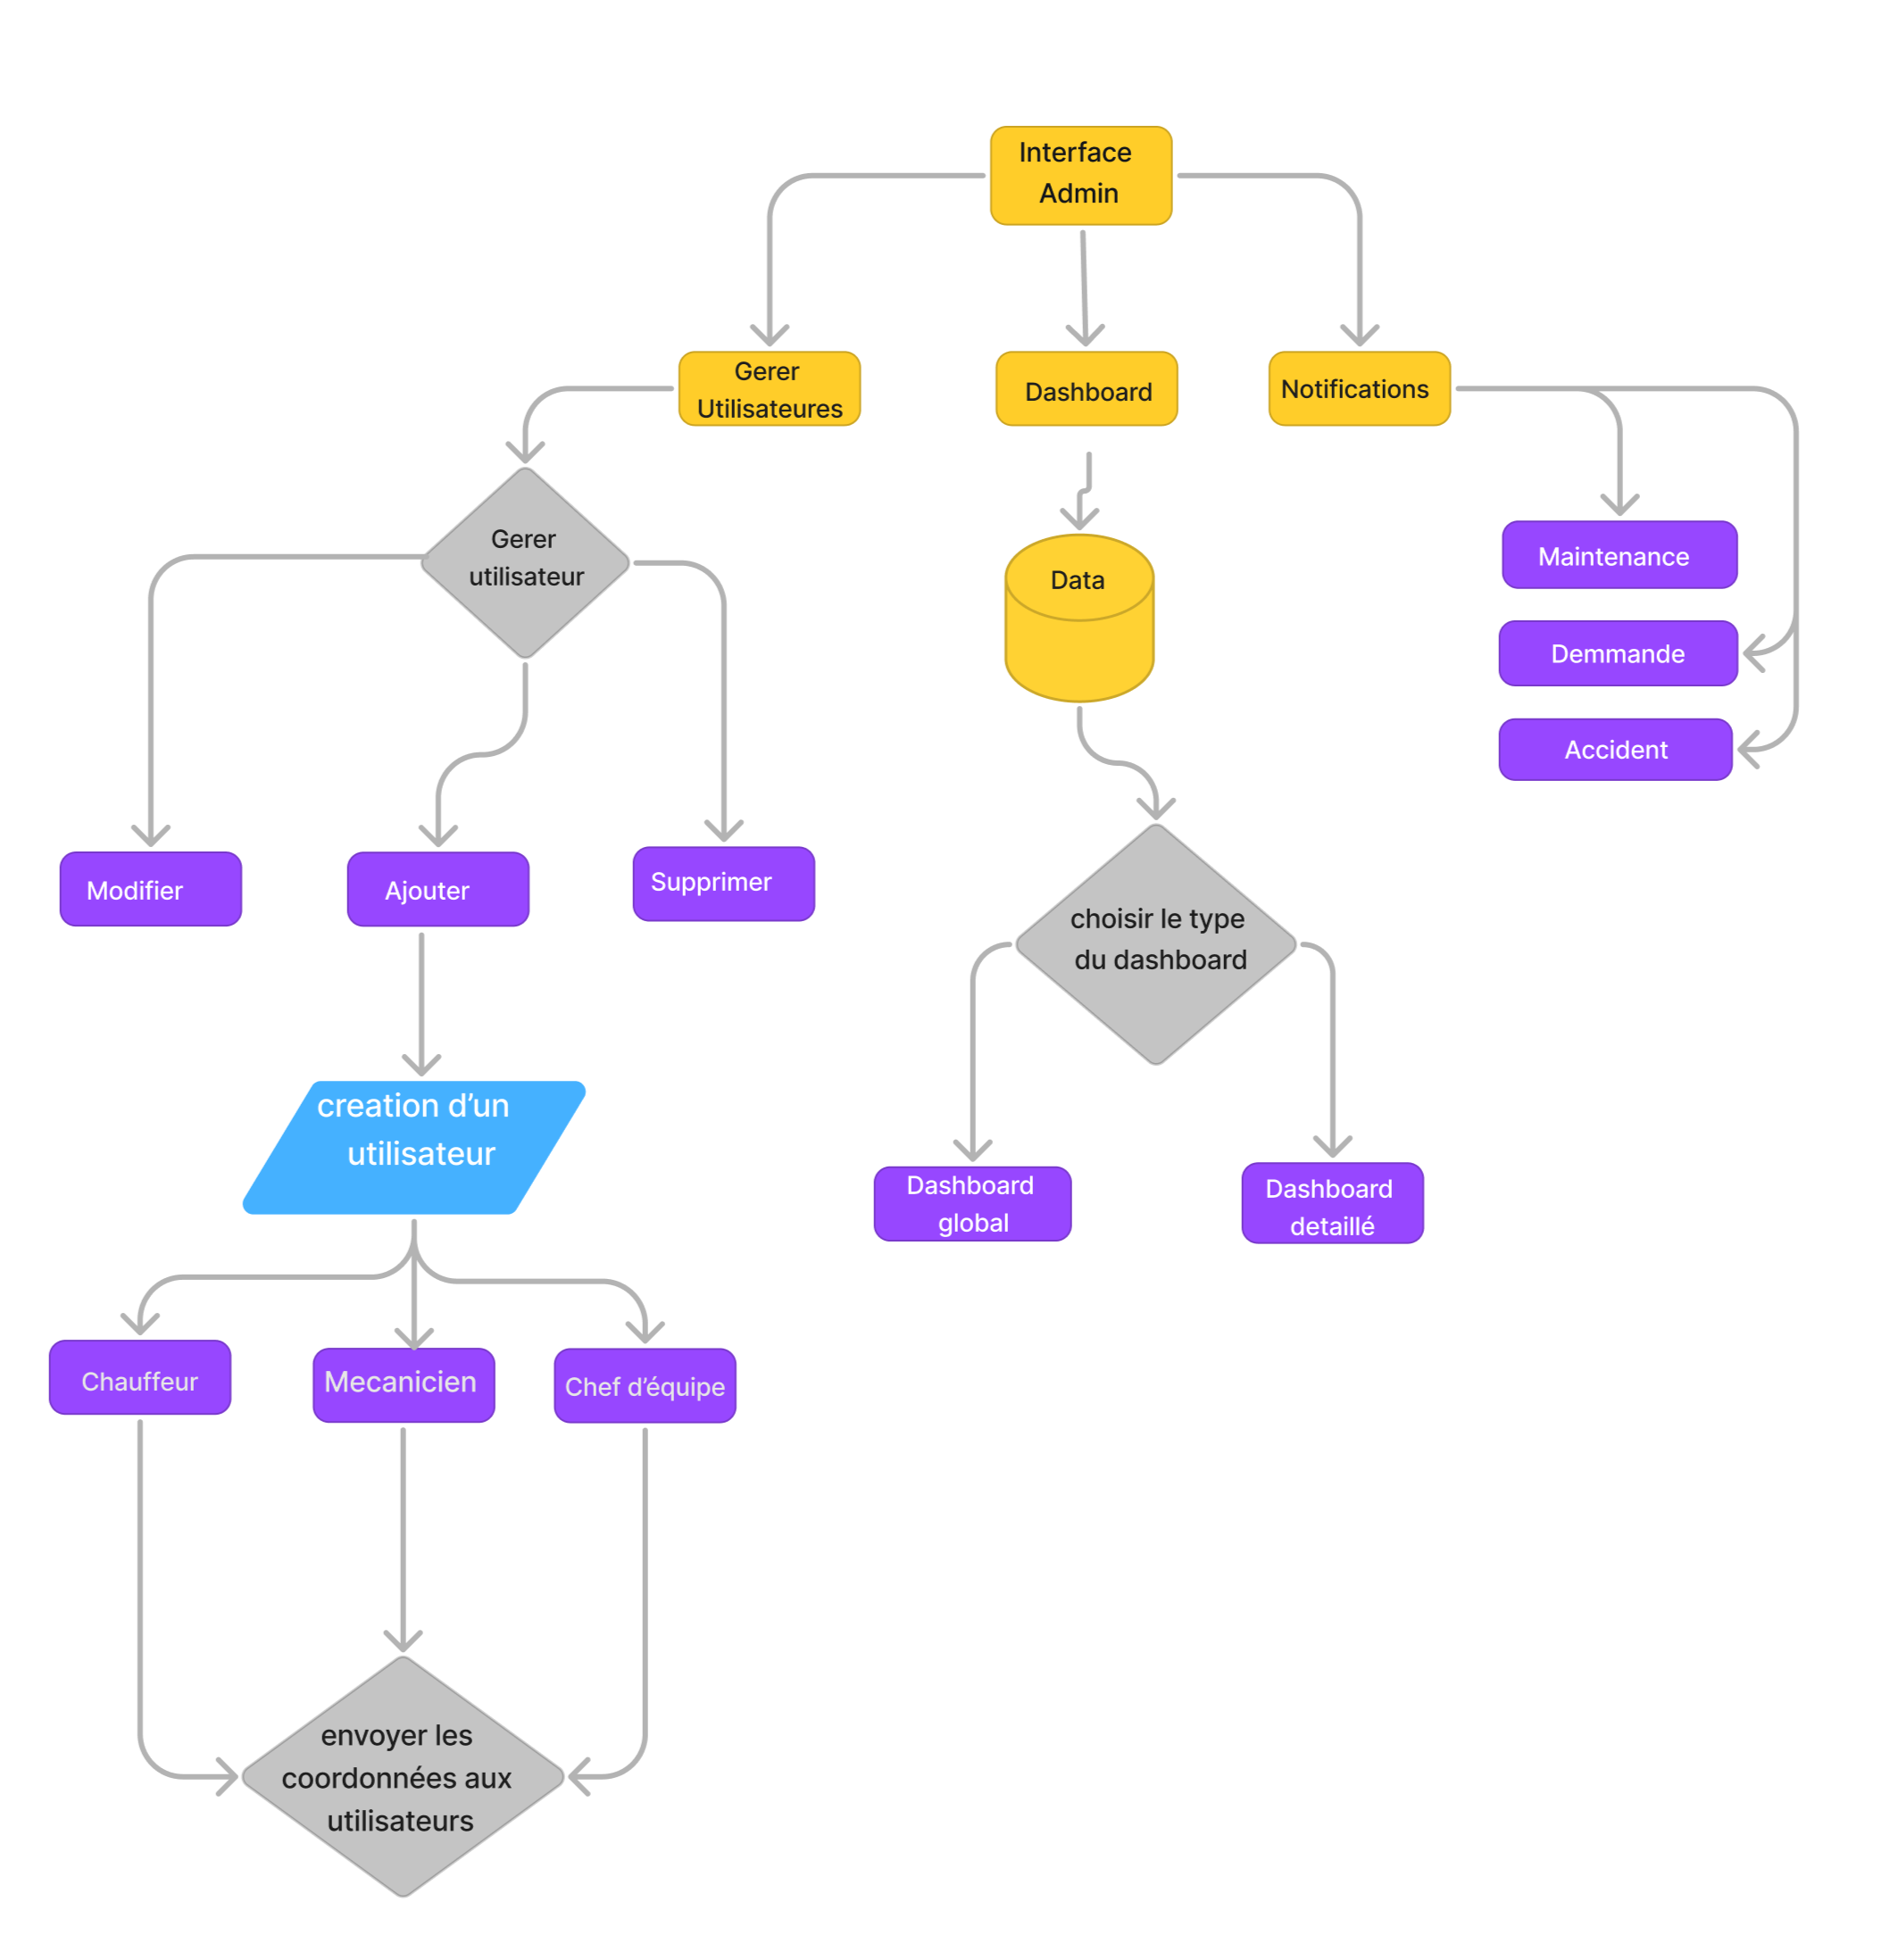
\includegraphics[width=1\textwidth,height=17cm]{chap2.images/org admin.png}
  \caption{Organigramme des interfaces du l'administrateur }
\end{figure}


\newpage
\subsubsection{Flux chauffeur}
\begin{figure}[htbp]
  \centering
  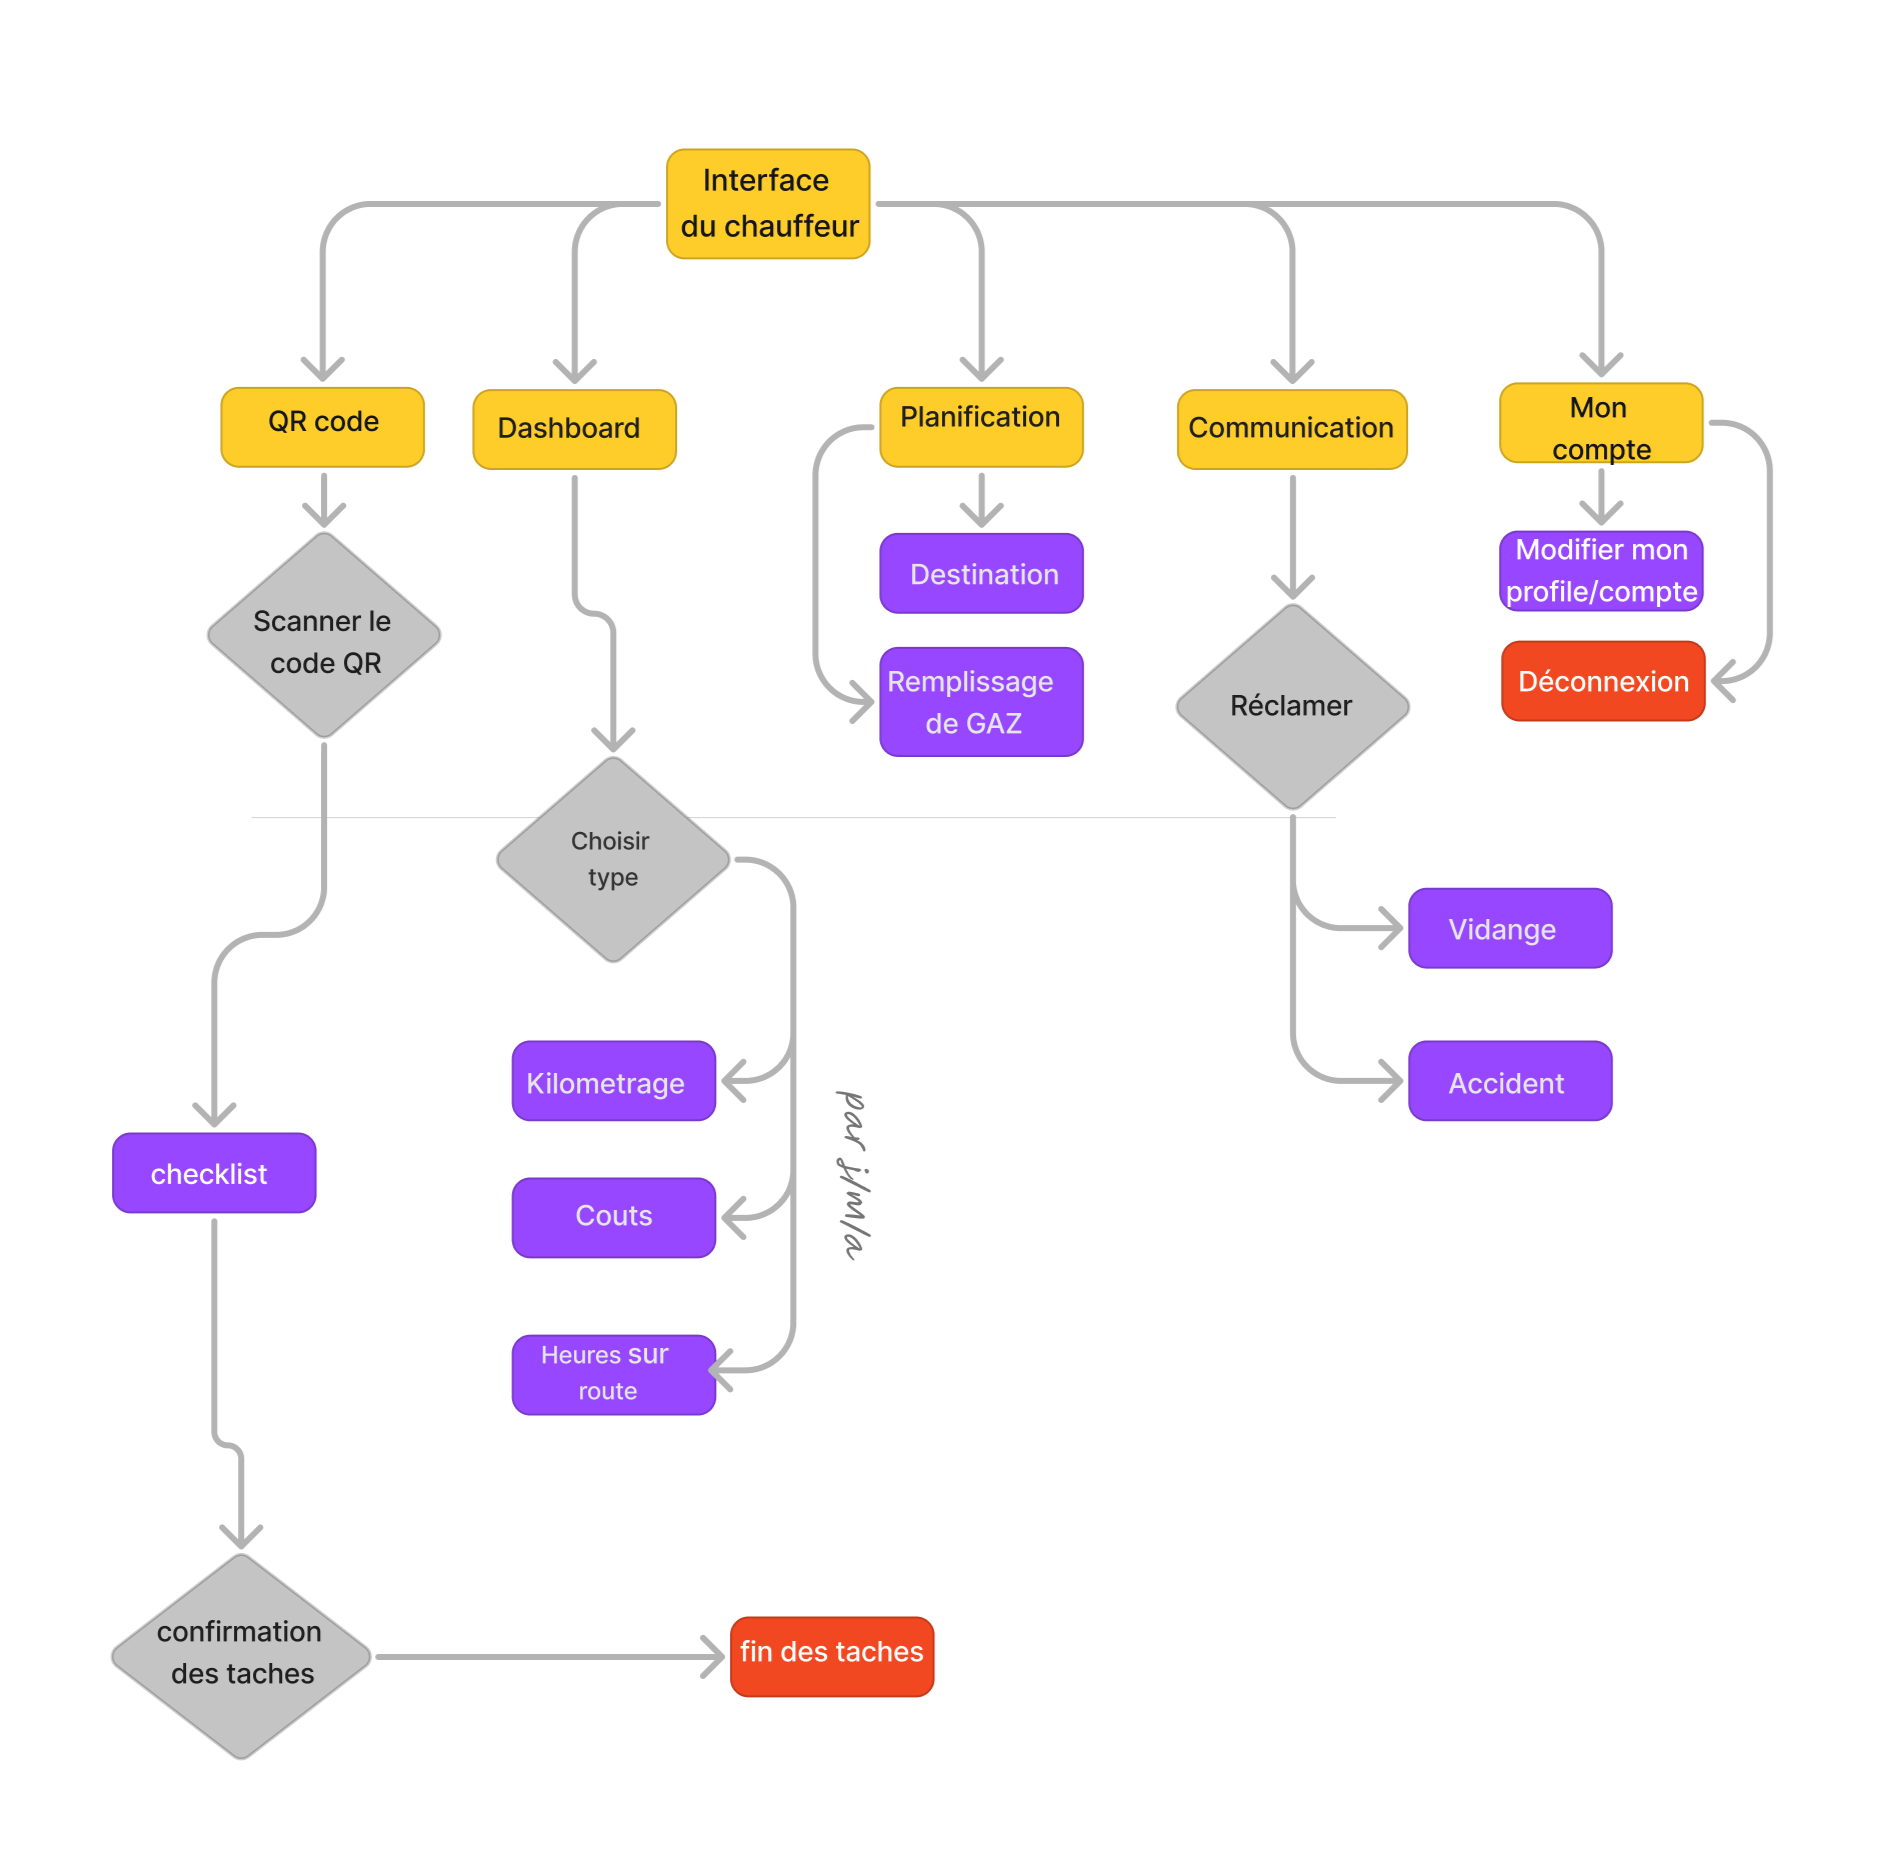
\includegraphics[width=1\textwidth,height=17cm]{chap2.images/org chauffeur.png}
  \caption{Organigramme des interfaces du chauffeur}
\end{figure}

\newpage
\subsubsection{Flux mécanicien}
\begin{figure}[htbp]
  \centering
  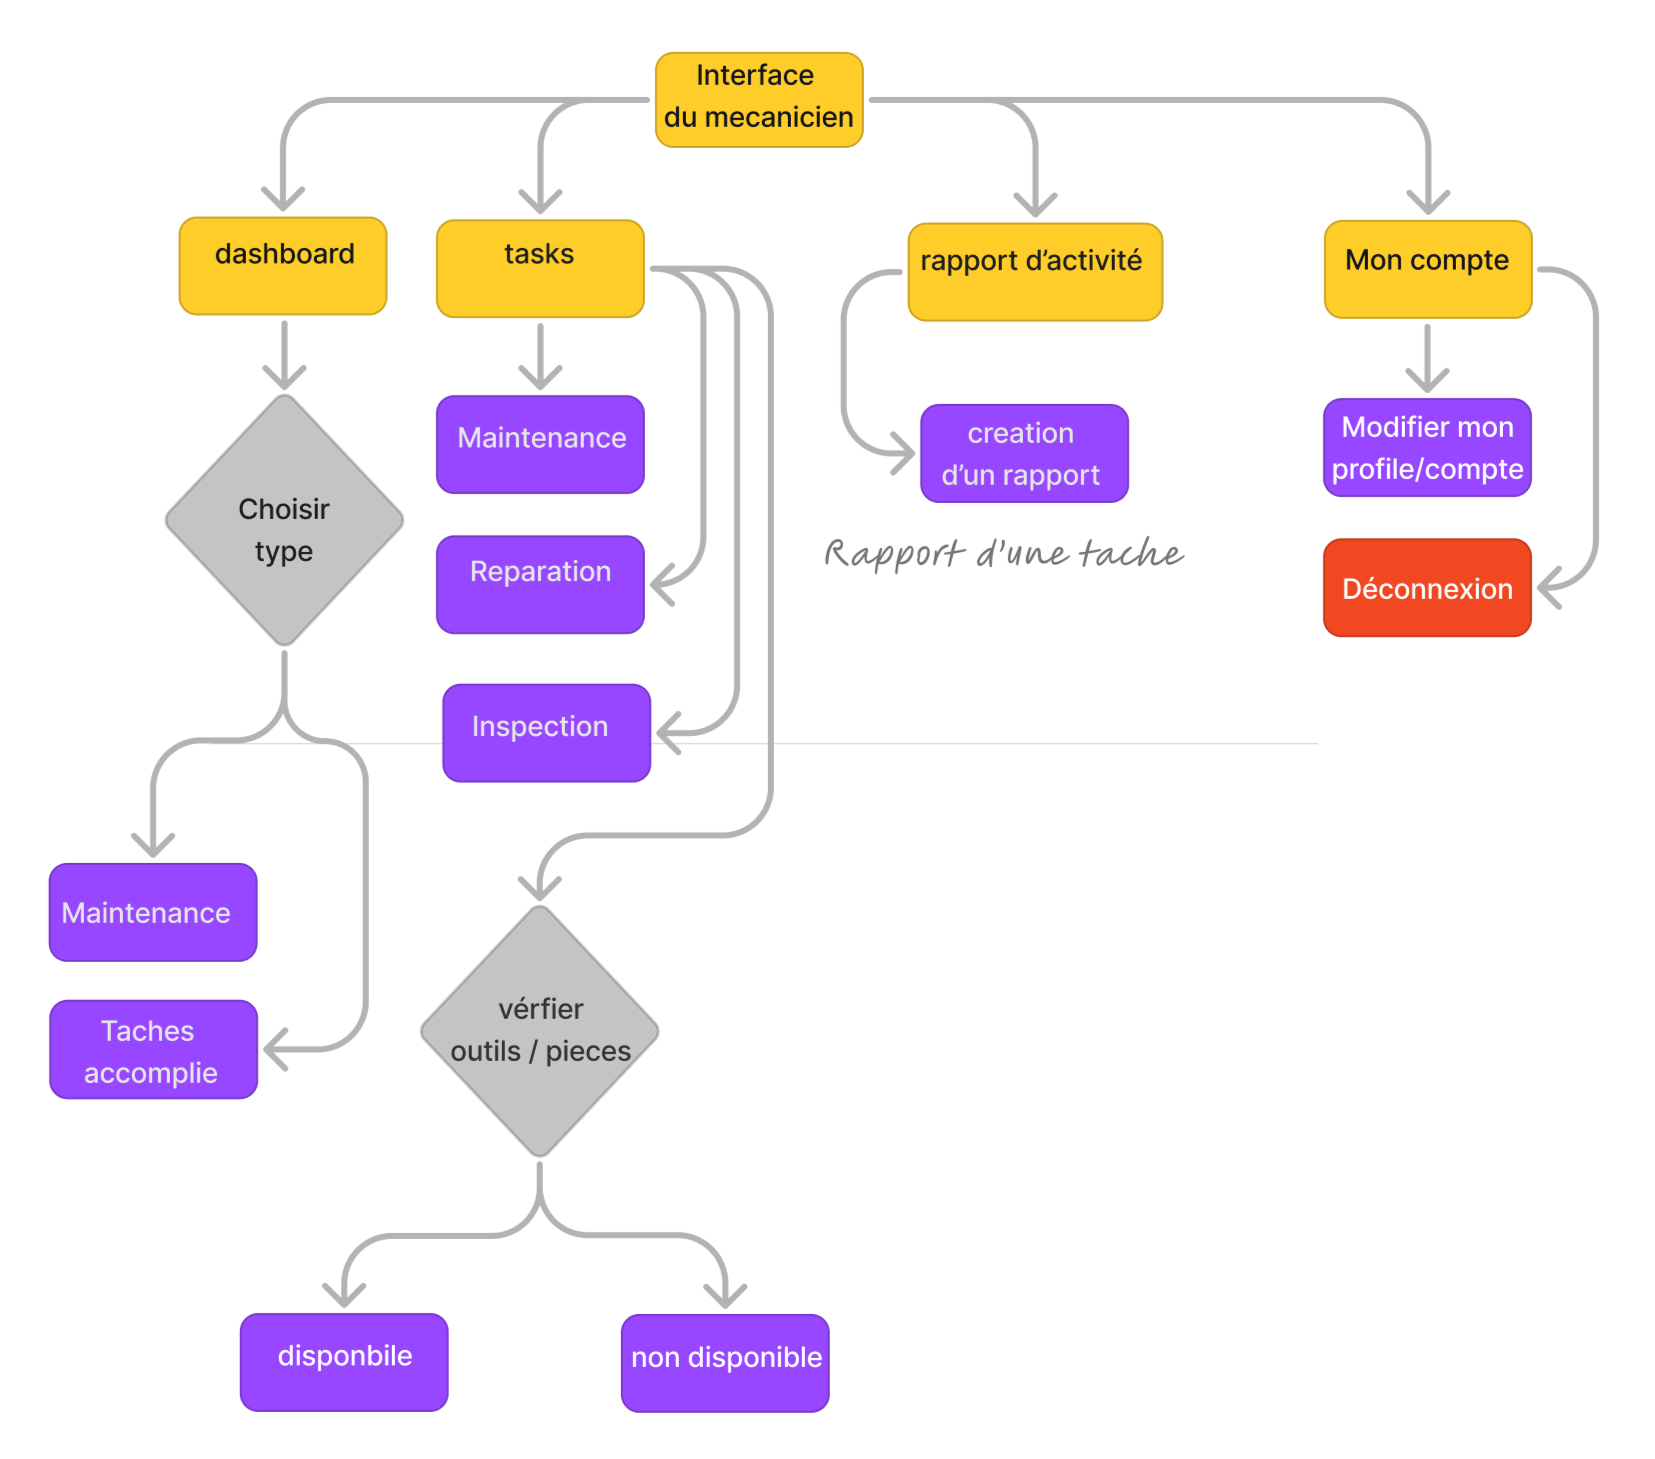
\includegraphics[width=1\textwidth,height=17cm]{chap2.images/org mecanicien.png}
  \caption{Organigramme des interfaces  du mécanicien}
\end{figure}

\newpage
\subsubsection{Flux chef d'équipe}
\begin{figure}[htbp]
  \centering
  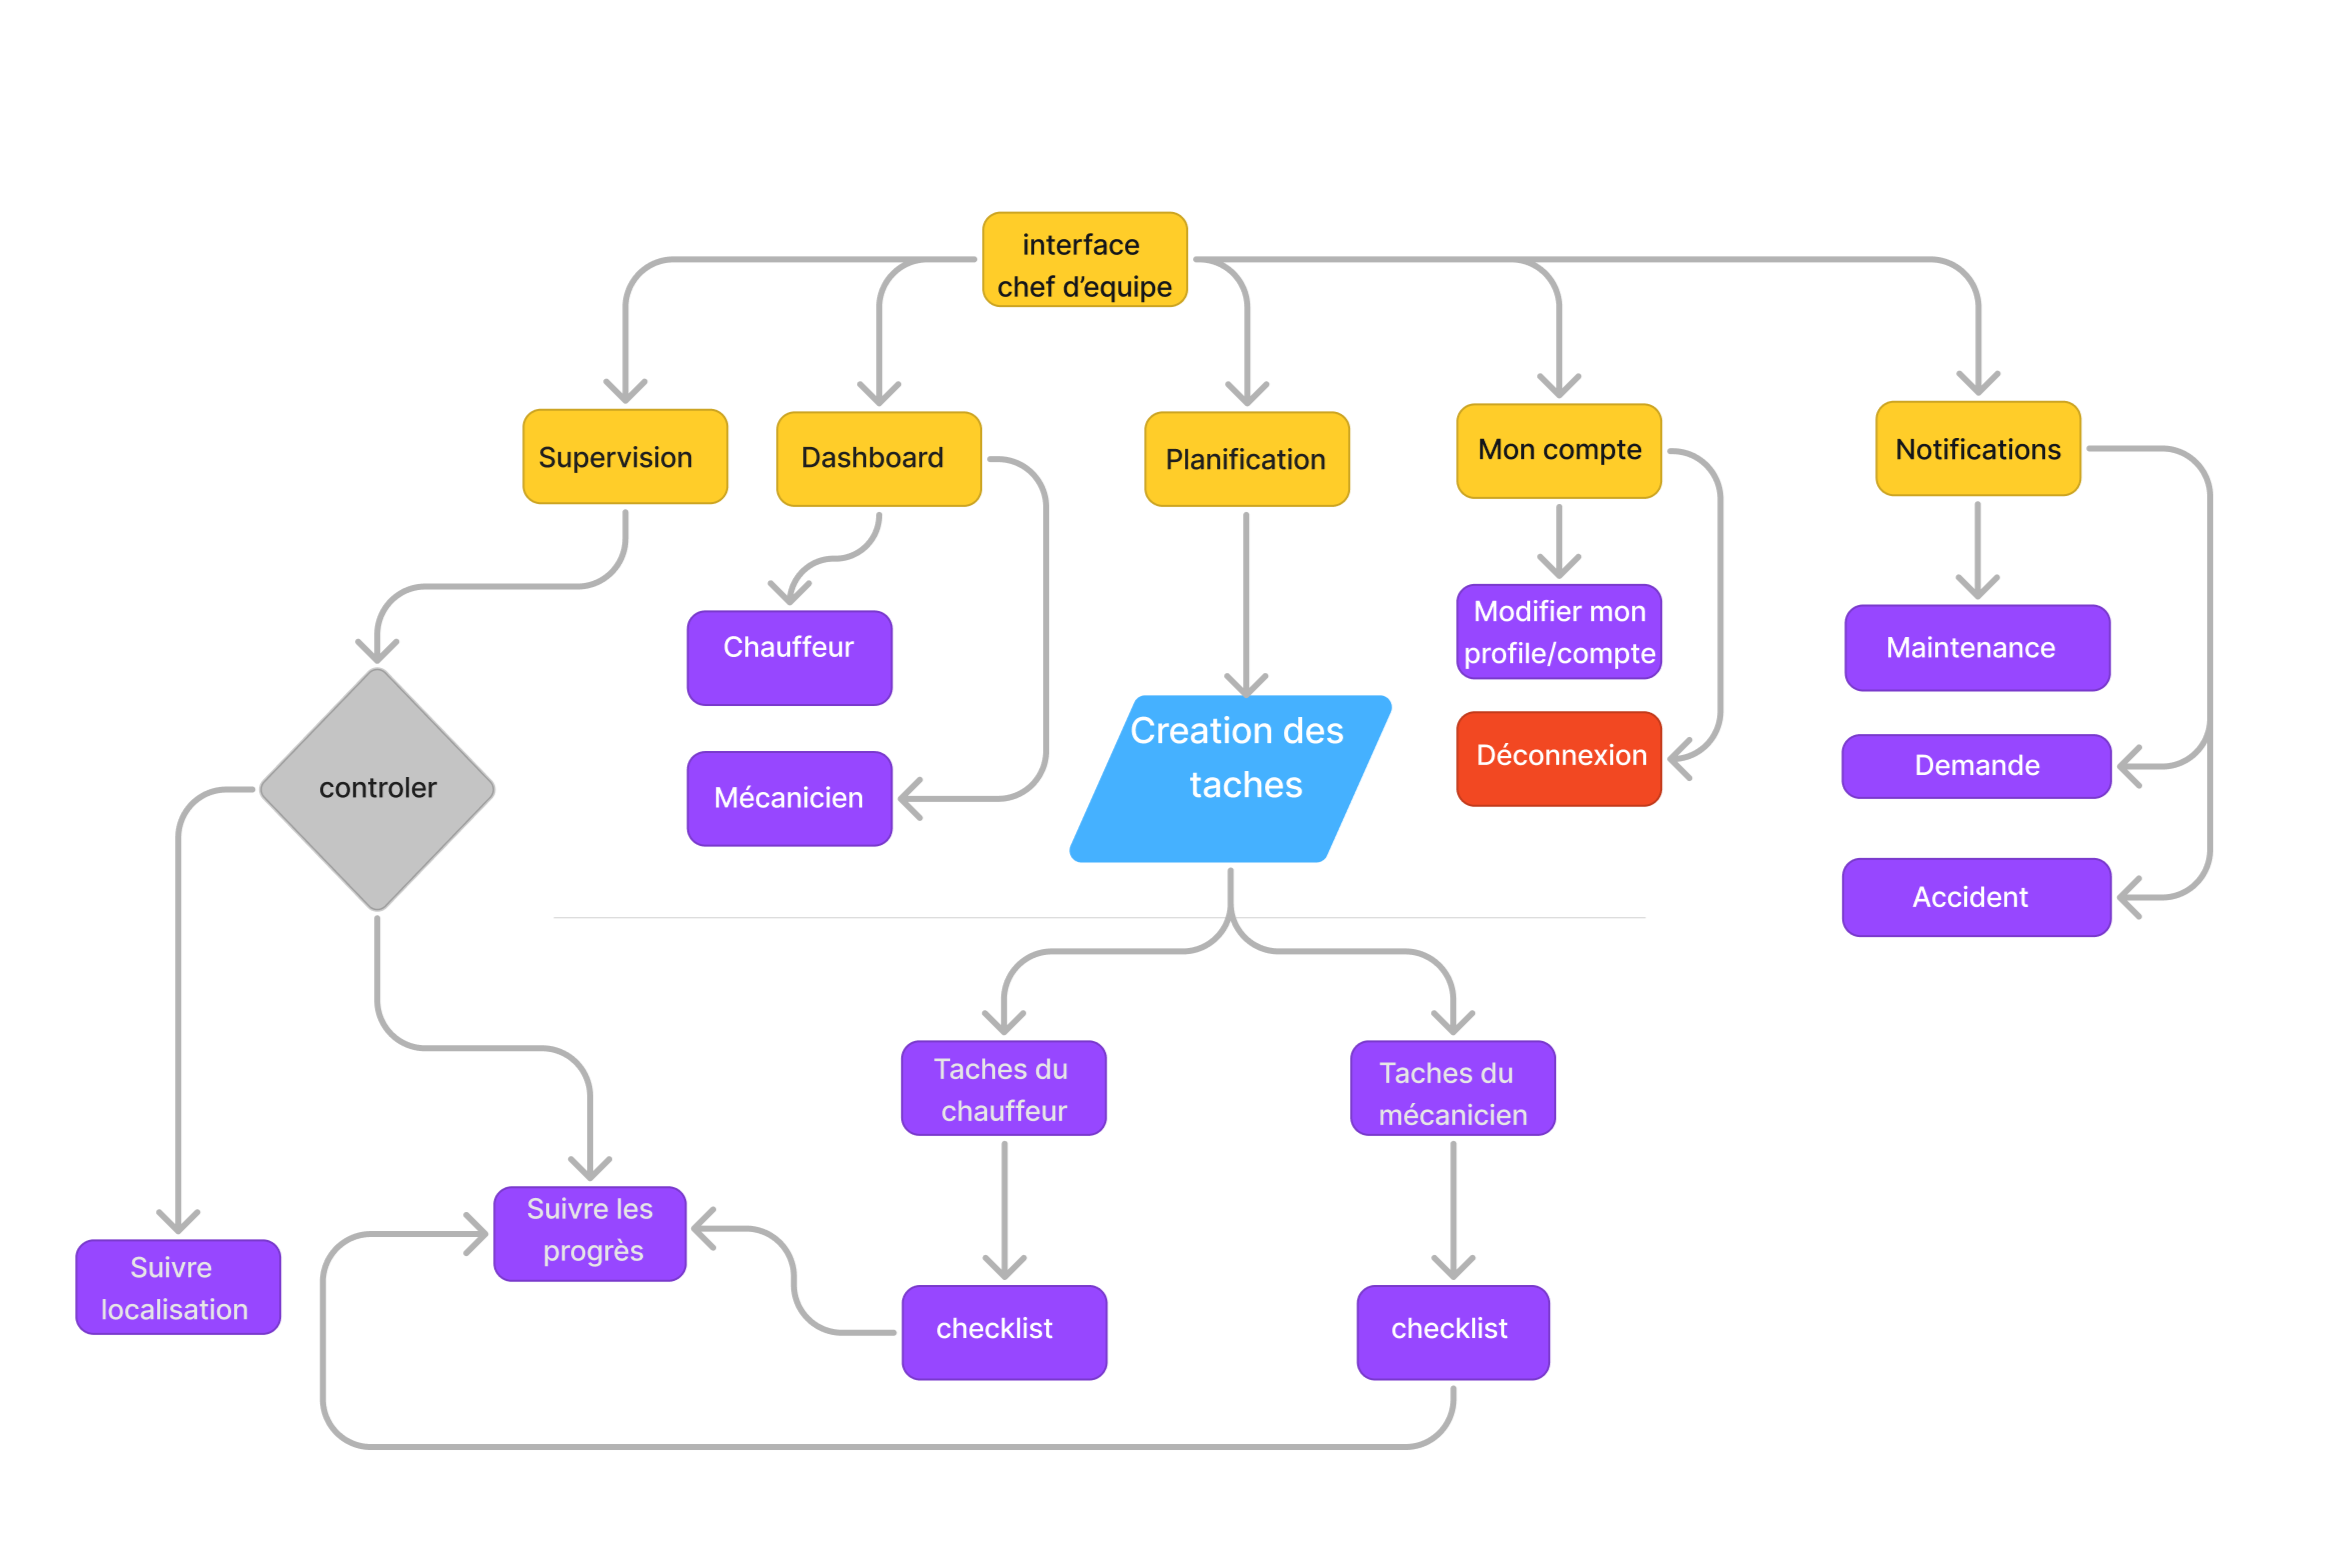
\includegraphics[width=1\textwidth,height=17cm]{chap2.images/org chef d'equipe.png}
  \caption{Organigramme des interfaces du chef d'équipe}
\end{figure}



%_________________________________________________________________________________________________________

\newpage
\subsection{Diagramme de classe du domaine}

La figure 2.21 montre le diagramme de classes du domaine de notre application.








%_________________________________________________________________________________________________________


\newpage
\subsection{Diagramme de Gantt }

Par cette figure 2.20 nous présentons une planification previsionnelle du projet .

\begin{figure}[ht!]
  \centering
  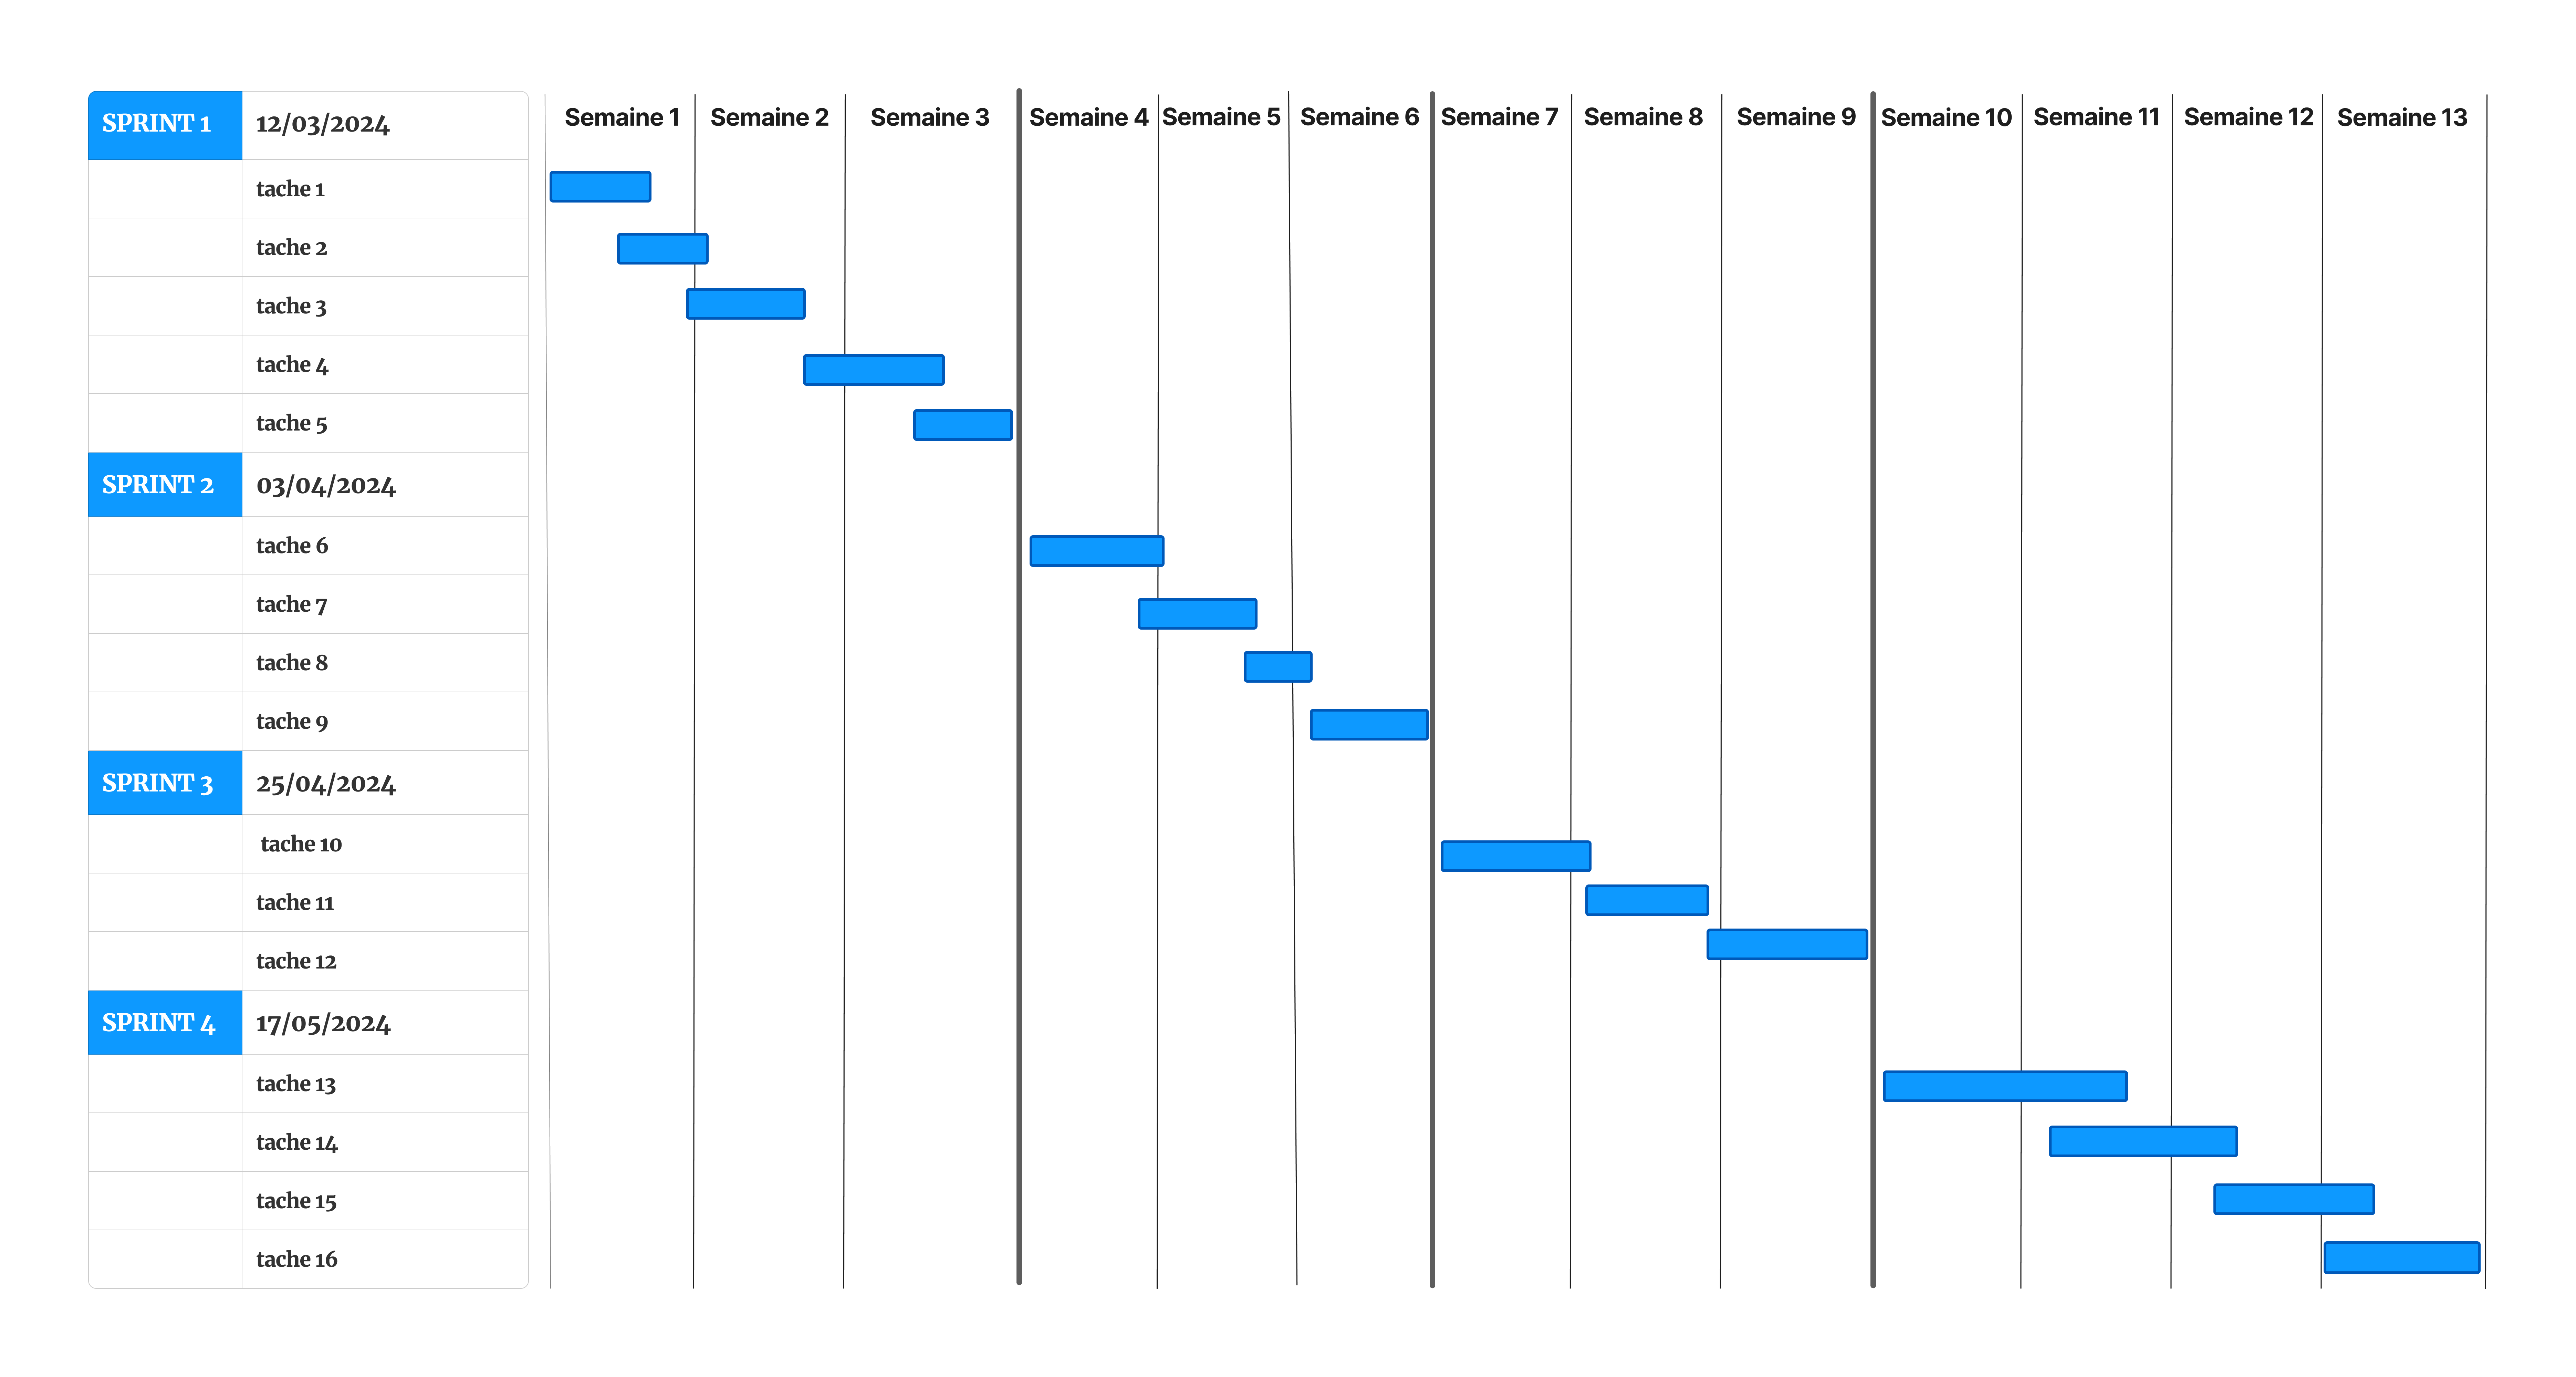
\includegraphics[width=1\textwidth,height=11cm]{chap2.images/diagramme de gantt.png}
  \caption{Diagramme de Gantt}
\end{figure}






%_________________________________________________________________________________________________

\section*{Conclusion}
\addcontentsline{toc}{section}{Conclusion}
\bigskip
\begin{sloppypar}
  Durant ce chapitre, en plus de l'identification  des acteurs, des besoins fonctionnels et non fonctionnels de notre application,  nous avons exposé le premier artéfact de la méthodologie Scrum à savoir le Backlog du produit qui comporte la liste des exigences fonctionnelles et techniques de notre application. Nous avons également identifié les différents rôles au sein de l'équipe du projet et en fin nous avons  exploré le flux utilisateurs de notre application, mettant en évidence les différentes interactions entre les utilisateurs et les fonctionnalités clés de l'application.
  Dans le chapitre suivant, nous allons commencer notre premier sprint.
\end{sloppypar}







\chapter{  Sprint 1 : Gestion des accès}

\section*{Introduction}
\addcontentsline{toc}{section}{Introduction}
Dans ce sprint, l'équipe s'est concentrée sur la mise en place des fonctionnalités de base, notamment l'authentification des utilisateurs, la déconnexion sécurisée, la gestion des utilisateurs et la définition des rôles. Ces éléments sont essentiels pour assurer la sécurité et la convivialité de l'application, ainsi que pour permettre une gestion efficace des utilisateurs et de leurs autorisations.

%________________________________________________________________________________________________________________

\section{Backlog du sprint 1}
Le backlog du sprint présente un ensemble des fonctionnalités extraites par l’équipe scrum à partir du backlog de produit et qui vont être réalisés pendant ce sprint. Les tâches à achever
pendant notre premier sprint sont présentées dans le tableau 3.1 suivant :

\begin{table}[H]
  \centering
  \renewcommand{\arraystretch}{1}
  \begin{tabular}{|c|c|p{7.5cm}|c|}
    \hline
    \textbf{ID}  & \textbf{Fonctionnalités} & \centering \textbf{User Story}                                                                                             & \textbf {Story points} \\
    \hline
    \textbf{US1} & Authentification         & En tant qu'admin, chauffeur, chef d'équipe et mécanicien je veux m'authentifier pour que j'accède à mon espace.            & 3                      \\
    \hline
    \textbf{US2} & Déconnexion              & En tant qu'admin, chauffeur, chef d'équipe et mécanicien je veux me déconnecter pour que je quitte l'application.          & 1                      \\
    \hline
    \textbf{US3} & Modification profil      & En tant qu'admin, chauffeur, chef d'équipe et mécanicien je veux modifier mon profil pour modifier photo et mots de passe. & 3                      \\
    \hline
    \textbf{US4} & Gestion des utilisateurs & En tant qu'admin je veux Gérer les utilisateurs pour que je puisse les ajouter,modifier et supprimer .                     & 5                      \\
    \hline
    \textbf{US5} & Gestion des rôles        & En tant qu'admin, je veux pouvoir gérer les rôles et les autorisations des utilisateurs.                                   & 2                      \\
    \hline
  \end{tabular}
  \caption{Backlog du sprint 1}

\end{table}

%__________________________________________________________________________________________________________________________________________________________________________________
\newpage
\section{Analyse et conception}
La section "Analyse et Conception" présente les méthodes de conception et la structure de notre application. Elle présente les diagrammes de cas d'utilisation, qui identifient les interactions des utilisateurs avec le système, les diagrammes de séquences système, qui illustrent l'ordre des opérations et la coordination entre les composants du système, et les diagrammes de classes participantes, qui dépeignent la structure objet et les relations entre les classes. Ces diagrammes sont essentiels pour comprendre le fonctionnement interne et l'architecture de l'application, afin de  répondre aux besoins des utilisateurs

%________________________________________________________________________________________________________________

\subsection{Diagramme de cas d’utilisation du sprint 1}

Ce diagramme illustre les différentes interactions que les utilisateurs peuvent avoir avec notre application. Il sert à identifier clairement les fonctionnalités accessibles par chaque type d'utilisateur et à définir les exigences système nécessaires pour ces interactions.

\begin{figure}[ht!]
  \centering
  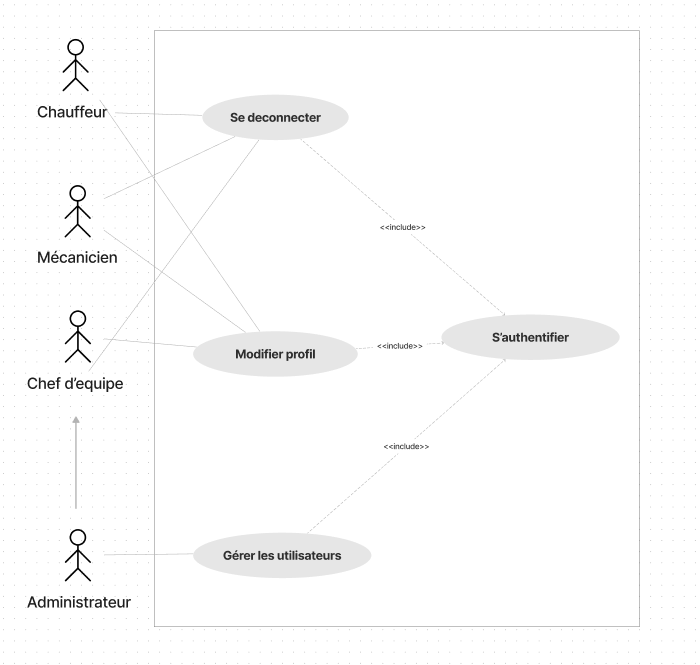
\includegraphics[width=1\textwidth,height=14cm]{chap3.images/usecase global sprint 1.png}
  \caption{Diagramme de cas d’utilisation global du sprint 1}

\end{figure}

%________________________________________________________________________________________________________________



\newpage
\subsection{Description textuelle du cas d’utilisation “S’authentifier”}

\begin{table}[H]
  \centering
  \renewcommand{\arraystretch}{1.2}
  \begin{tabular}{|p{4cm}|p{9cm}|}
    \hline
    \textbf{Cas d'utilisation}   & S'authentifier                                                                                                                   \\
    \hline
    \textbf{Acteur}              & Administrateur, Chef d’équipe, Chauffeur et Mécanicien                                                                           \\
    \hline
    \textbf{Pré-condition}       & L'utilisateur accède à l'interface d'authentification de l'application.                                                          \\
    \hline
    \textbf{Post-condition}      & L'utilisateur est authentifié et accède à son espace sécurisé dans l'application.                                                \\
    \hline
    \textbf{Scenario nominal}    & 1- L'utilisateur saisit son identifiant et son mot de passe.\newline

    2- L'utilisateur appuie sur le bouton de confirmation.\newline

    3- Le système vérifie les informations d'identification fournies par l'utilisateur. \newline

    4- L'utilisateur est redirigé vers son espace sécurisé dans l'application.                                                                                      \\


    \hline
    \textbf{Scénario alternatif} & A1 identifiants / mot de passe erroné :                                                                                 \newline

    l'enchainement A1 démarre au point 3 du scénario nominal. \newline

    4- un message d'erreur va etre afficher. \newline

    Le scénario nominal reprend au point 1.                                                                                                                         \\
    \hline
  \end{tabular}
  \caption{Description textuelle du cas d’utilisation “S’authentifier”}

\end{table}
%________________________________________________________________________________________________________________

\newpage
\subsection{Diagramme de séquence système du cas d’utilisation «S’authentifier»}
Un diagramme de séquences système est une représentation graphique qui illustre les interactions entre les acteurs ou les composants d'un système informatique pour accomplir une série d'actions ou de processus. Il met en évidence la chronologie des échanges de messages entre ces entités, fournissant ainsi une vue détaillée de la façon dont le système fonctionne pour atteindre ses objectifs.

\bigskip
\begin{figure}[ht!]
  \centering
  \includegraphics[width=1\textwidth,height=18cm]{chap3.images/Dss S’authentifier.png}
  \caption{Diagramme de séquence système du cas d’utilisation « S’authentifier » }

\end{figure}

%________________________________________________________________________________________________________________
\newpage

\subsection{Raffinement du cas d'utilisation « Gérer les utilisateurs »}

\begin{figure}[ht!]
  \centering
  \includegraphics[width=1\textwidth,height=6cm]{chap3.images/gerer raf sprint 1.png}
  \caption{Analyse de cas d’utilisation « Gérer les utilisateurs »}

\end{figure}

%________________________________________________________________________________________________________________


\subsection{Description textuelle du cas d’utilisation “Ajouter utilisateur”}
\begin{table}[H]
  \centering
  \renewcommand{\arraystretch}{1.1}
  \begin{tabular}{|p{4cm}|p{9cm}|}
    \hline
    \textbf{Cas d'utilisation}   & Ajouter Utilisateur                                                                                           \\
    \hline
    \textbf{Acteur}              & Administrateur                                                                                                \\
    \hline
    \textbf{Pré-condition}       & L'administrateur est authentifié dans le système .                                                            \\
    \hline
    \textbf{Post-condition}      & Le nouvel utilisateur est ajouté avec succès dans le système et peut accéder aux fonctionnalités appropriées. \\
    \hline
    \textbf{Scenario nominal}    & 1- L'administrateur accède à l'interface de gestion des utilisateurs.\newline

    2- L'administrateur ajoute un nouvel utilisateur en saisissant ses informations dans un formulaire dédié.\newline

    3- Le système vérifie les informations saisies.\newline
    
    4- Le nouvel utilisateur est ajouté à la base de données.\newline

    5- Le système envoie un e-mail au nouvel utilisateur contenant ses informations de connexion pour accéder au système.                        \\
    \hline
    \textbf{Scénario alternatif} & A1 Erreur de saisie des informations : \newline

    l'echainement A1 démarre au point 3 du scenario nominal.                                                                                     \\
  \end{tabular}

\end{table}


\begin{table}[H]
  \centering
  \renewcommand{\arraystretch}{1.1}
  \begin{tabular}{|p{4cm}|p{9cm}|}

     & 4- Le système affiche un message pour verifier les informations saisies.\newline

    Le scénario nominal reprend au point 2.                                             \\

    \hline
  \end{tabular}
  \caption{Description textuelle du cas d’utilisation “Ajouter utilisateur”}



\end{table}

%________________________________________________________________________________________________________________

\subsection{Diagramme de séquence système du cas d’utilisation «Ajouter utilisateur»}

\begin{figure}[ht!]
  \centering
  \includegraphics[width=1\textwidth,height=17.5cm]{chap3.images/DSS ajouter utilisateur.png}
  \caption{ Diagramme de séquence système du cas d’utilisation «Ajouter utilisateur» }
\end{figure}
%________________________________________________________________________________________________________________
%________________________________________________________________________________________________________________
\newpage
\section{Diagramme de classes du sprint 1}

\begin{figure}[ht!]

  \centering
  \includegraphics[width=1\textwidth,height=9cm]{chap3.images/class sprint 1.png}
  \caption{Diagramme de classes du sprint 1}

\end{figure}

%________________________________________________________________________________________________________________
\newpage
\section{ Réalisation}

Dans cette section, nous mettons en lumière les interfaces  de l'application que nous avons développée. À travers des captures d'écran détaillées, nous illustrons les fonctionnalités clés mises à disposition des utilisateurs, démontrant ainsi l'application pratique des concepts et des designs discutés dans les sections précédentes.



\subsection{Authentification}
Cette interface permet au utilisateurs de se connecter à l'application . L'utilisateur est accueilli par un formulaire de connexion simple, comprenant des champs pour saisir son identifiant et son mot de passe. Une fois les informations d'identification saisies, l'utilisateur peut appuyer sur le bouton  'confirmer' pour accéder à son espace sécurisé, si les informations d'identification saisies sont incorrectes, le système affiche un message d'erreur. \\


\begin{figure}[ht!]
  \centering
  \includegraphics[width=0.9\textwidth,height=6.5cm]{chap3.images/Authentification web.png}
  \caption{Interface d'authentification Web }

\end{figure}
\begin{figure}[ht!]
  \centering
  \includegraphics[width=0.9\textwidth,height=6.5cm]{chap3.images/authentification échoué.png}
  \caption{Echec de connexion }

\end{figure}

%________________________________________________________________________________________________________________

\newpage

\begin{figure}[htbp]
  \centering
  \begin{minipage}{0.45\textwidth}
    \centering
    \includegraphics[width=0.7\textwidth,height=8cm]{chap3.images/authentfication mob.png}
    \caption{\centering{Interface d'authentification Mobile}}

  \end{minipage}
  \hfill
  \begin{minipage}{0.45\textwidth}
    \centering
    \includegraphics[width=0.7\textwidth,height=8cm]{chap3.images/echec authentification mob.png}
    \caption{Echec de connexion }

  \end{minipage}
\end{figure}


\vspace{1.2cm}
%________________________________________________________________________________________________________________

\subsection{ Profil}

Permet à l'administrateur, chef d'équipe, chauffeur et mécanicien de changer leur photo de profil et leur mot de passe.

\begin{figure}[h!]
  \centering
  \begin{minipage}[t]{0.59\textwidth}
    \centering
    \includegraphics[width=1\textwidth, height=6cm]{chap3.images/modifier profil (web).png}
    \caption{Interface de profil  - Web}
  \end{minipage}
  \hfill
  \begin{minipage}[t]{0.39\textwidth}
    \centering
    \includegraphics[width=0.7\textwidth, height=7.5cm]{chap3.images/modifier profil mobile.png}
    \caption{\centering{Interface de profil - Mobile}}
  \end{minipage}
\end{figure}

%%%%%%%%%%%%%%%%%%%%%%%%%%%%%%%%%%%%%%%%%
\newpage
\subsection{Gestion des utilisateurs}
Lorsque l'administrateur accède à cette interface, il est présenté avec un tableau répertoriant tous les utilisateurs de l'application. Chaque ligne du tableau représente un utilisateur et affiche des informations telles que le nom, l'adresse e-mail et le rôle. L'administrateur a la possibilité de supprimer un utilisateur en cliquant sur l'icône de suppression correspondante dans la ligne de l'utilisateur. De plus, en cliquant sur l'icône de modification, l'administrateur peut mettre à jour les informations d'un utilisateur existant.
\bigskip

\begin{figure}[ht!]
  \centering
  \includegraphics[width=0.9\textwidth]{chap3.images/Gérer user.png}
  \caption{Interface de gestion des utilisateurs}

\end{figure}

%%%%%%%%%%%%%%%%%%%%%%%%%%%%%%%%%%%%%%%%%

\subsection{Création d'un nouvel utilisateur}
Lorsque l'administrateur clique sur le bouton "Ajouter Utilisateur" dans l'interface précédente, un formulaire d'ajout d'utilisateur s'affiche à l'écran. Ce formulaire permet à l'administrateur de saisir les informations nécessaires pour créer un nouvel utilisateur, telles que le nom, l'adresse e-mail et le mot de passe initial. L'administrateur peut également sélectionner le rôle de l'utilisateur parmi les options disponibles. Une fois que toutes les informations requises sont fournies, l'administrateur peut soumettre le formulaire pour créer un nouvel utilisateur dans le système.\\

\newpage
\begin{figure}[ht!]
  \centering
  \includegraphics[width=0.9\textwidth,height=7cm]{chap3.images/creer user.png}
  \caption{Interface de création d'un nouvel utilisateur}

\end{figure}
%________________________________________________________________________________________________________________
\section{Rétrospective}
Dans cette section de rétrospective, nous examinerons de près les performances de notre équipe pendant le Sprint 1 en utilisant deux outils essentiels de la méthodologie Scrum : le burndown chart et le task board. Ces outils nous permettent de visualiser et d'évaluer notre progression tout au long du sprint.

\subsection{Burdown Chart}
Le burndown chart est un outil essentiel utilisé dans la gestion de projet agile pour suivre la progression des tâches. Il illustre graphiquement la quantité de travail restant à accomplir par l'équipe au cours du sprint. Dans notre cas, nous avons planifié un sprint de 3 semaines, avec une moyenne de 5 heures de travail par jour.

\begin{figure}[ht!]
  \centering
  \includegraphics[width=1\textwidth, height=6.5cm]{chap3.images/burndown chart sprint 1.png}
  \caption{ Burdown Chart du Sprint 1}

\end{figure}
%%%%%%%%%%%%%%%%%%%%%%%%%%%%%%%%%%%%%%%%%

\newpage
\subsection{Task Bord}

La figure 3.14 présente le "Task Bord" correspondant au 6ème jour du sprint 1.

\begin{figure}[ht!]
  \centering
  \includegraphics[width=0.9\textwidth, height=8cm]{chap3.images/task board sprint 1.png}
  \caption{ Task board du Sprint 1 }

\end{figure}
%_______________________________________________________________________________________________
\section{Tests unitaires}
Dans cette section, nous utiliserons l'outil Postman pour effectuer des tests unitaires sur notre application. Les tests unitaires consistent à vérifier le bon fonctionnement de chaque unité de code de manière isolée. Nous définirons des scénarios de test, configurerons des requêtes HTTP dans Postman, et écrirons des scripts pour valider les résultats renvoyés par chaque unité de code. Ces tests nous permettront de détecter les erreurs dès le stade de développement .\\\\
%_______________________________________________________________________________________________
\bigskip
\textbf{Test unitaires du cas d’utilisation « S'authentifier » :}\\
Nous présentons ci-dessous le code source et le résultat de deux cas de test :

1. Toutes les données sont valides.\newline
2. Mots de passe incorrecte .

\begin{figure}[ht!]
  \centering
  \includegraphics[width=0.7\textwidth, height=3.5cm]{chap3.images/code source test.png}
  \caption{ Code souce du test unitaire du cas d’utilisation «S’authentifier » }

\end{figure}

\newpage
\begin{figure}[ht!]
  \centering
  \includegraphics[width=0.7\textwidth, height=6.5cm]{chap3.images/cas1.png}
  \caption{ Resultat du premier test }

\end{figure}

\begin{figure}[ht!]
  \centering
  \includegraphics[width=0.7\textwidth, height=6.5cm]{chap3.images/cas2.png}
  \caption{ Resultat du deuxieme test }

\end{figure}
%_______________________________________________________________________________________________

\section*{Conclusion}
\addcontentsline{toc}{section}{Conclusion}
\bigskip
\begin{sloppypar}
  Dans ce chapitre, nous avons examiné en détail le premier Sprint, en décrivant le contenu du Sprint Backlog, le diagramme de cas d'utilisation et les séquences système des cas d'utilisation principaux. Nous avons également illustré quelques fonctionnalités de l'application à travers un scénario, et présenté d'autres outils de Scrum comme le Task Board et le burndown Chart. Dans le prochain chapitre, nous continuerons à explorer les fonctionnalités du deuxième Sprint.
\end{sloppypar}


\chapter{  Sprint 2 : Gestion des Tâches }

\section*{Introduction}
\addcontentsline{toc}{section}{Introduction}

Dans ce sprint, nous nous concentrons sur le développement des fonctionnalités de création et de consultation des tâches dans notre application. Nous avons élaboré un backlog, des cas d'utilisation, des diagrammes de séquence et des descriptions textuelles pour guider notre travail. Nous avons également conçu un diagramme de classe participantes pour planifier l'implémentation des fonctionnalités, ainsi que des captures d'écran des interfaces utilisateur. Nous examinerons également le burndown chart et le task board pour suivre l'avancement du sprint et discuterons de la mise en œuvre des tests unitaires pour garantir la qualité du code.
%________________________________________________________________________________________________________________

\section{Backlog du sprint 2}


\begin{table}[H]
  \centering
  \renewcommand{\arraystretch}{1} % Facteur d'étirement des lignes
  \begin{tabular}{|c|c|p{7.8cm}|c|}
    \hline
    \textbf{ID}   & \textbf{Fonctionnalités} & \centering \textbf{User Story}                                                                                                                      & \textbf {Story points} \\
    \hline
    \textbf{US6}  & Gestion des véhicules    & En tant qu'administrateur, je veux ajouter, supprimer et visualiser les véhicules pour que la gestion du parc soit efficace et à jour.              & 5                      \\
    \hline
    \textbf{US7}  & Créations des taches     & En tant que Chef d'équipe je veux Créer des taches pour les chauffeurs et les mécanicien.                                                           & 5                      \\
    \hline
    \textbf{US8}  & Consultation des taches  & En tant que Chauffeur je veux consulter la checklist pour que je puisse vérifier tous les éléments essentiels et confirmer l'exécution des tâches . & 3                      \\
    \hline
    \textbf{US9}  & Consultation des taches  & En tant que Mécanicien je veux Consulter les détails des interventions pour que je puisse obtenir toutes les informations sur les tâches assignées. & 3                      \\
    \hline
    \textbf{US10} & Validation des taches    & En tant que Chef d'équipe je veux valider les taches du mécanicien                                                                                  & 3                      \\
    \hline
  \end{tabular}
  \caption{Backlog du sprint 2}

\end{table}

%________________________________________________________________________________________________________________
\newpage
\section{Analyse et conception}

Dans cette section, nous détaillerons le processus d'analyse et de conception pour les fonctionnalités de création et de consultation des tâches.

%________________________________________________________________________________________________________________
\subsection{Diagramme de cas d’utilisation du sprint 2 }

\begin{figure}[h!]
  \centering
  \includegraphics[width=1\textwidth,height=10cm]{chap4.images/dcu global sprint 2.png}
  \caption{Diagramme de cas d’utilisation global du sprint 2}

\end{figure}

%________________________________________________________________________________________________________________
%________________________________________________________________________________________________________

\subsection{Raffinement du cas d'utilisation « Gérer les véhicules »}

\begin{figure}[h!]
  \centering
  \includegraphics[width=1\textwidth,height=6cm]{chap4.images/raf Gérer les véhicules.png}
  \caption{Raffinement de cas d’utilisation « Gérer les véhicues »}

\end{figure}


%________________________________________________________________________________________________________________

\subsection{Description textuelle du cas d’utilisation « Ajouter véhicules »}

\begin{table}[H]
  \centering
  \renewcommand{\arraystretch}{1.2} % Facteur d'étirement des lignes
  \begin{tabular}{|p{4cm}|p{9cm}|}
    \hline
    \textbf{Cas d'utilisation}   & Ajouter des Véhicules                                                                    \\
    \hline
    \textbf{Acteur}              & Administrateur                                                                           \\
    \hline
    \textbf{Pré-condition}       & 1- L'administrateur doit étre connecté .                                                 \\
    \hline
    \textbf{Post-condition}      & Le véhicule est ajouté à la base de données.                                             \\
    \hline
    \textbf{Scenario nominal}    & 1- L'administrateur accède à la section "Gestion des Véhicules" dans le système.\newline

    2- L'administrateur remplit les champs requis pour le nouveau véhicule.\newline

    3- L'administrateur clique sur "Confirmer" pour envoyer les informations du nouveau véhicule.\newline

    4- Le système vérifie que la plaque d'immatriculation n'est pas déjà utilisée.\newline

    5- Le système ajoute le véhicule à la base de données. \newline

    6- Le systéme affiche un message de confirmation indiquant que le véhicule a été ajouté avec succès.                    \\

    \hline
    \textbf{Scénario alternatif} & A1 Immatriculation déjà utilisée : \newline

    L'echainement A1 démarre au point 4 du scenario nominal.\newline

    5- Le système affiche un message pour vérifier les informations du nouveau véhicule .\newline

    Le scénario nominal reprend au point 2. \newline

    A2 Ajout du véhicule échoué dans la base de données :\newline

    L'echainement A2 démarre au point 5 du scenario nominal.                                                                \\
  \end{tabular}

\end{table}



\begin{table}[H]
  \centering
  \renewcommand{\arraystretch}{1.1} % Facteur d'étirement des lignes
  \begin{tabular}{|p{4cm}|p{9cm}|}


     & 6- Le système affiche un message que le véhicule n'a pas été ajouté à la base de données\newline

    Le scénario nominal reprend au point 4.                                                             \\

    \hline
  \end{tabular}
  \caption{Description textuelle du cas d’utilisation “Ajouter véhicules ”}

\end{table}

\subsection{Diagramme de séquence système du cas d’utilisation « Ajouter des véhicules »}
\begin{figure}[h!]
  \centering
  \includegraphics[width=1\textwidth,height=18cm]{chap4.images/dss ajouter vehicule.png}
  \caption{Raffinement de cas d’utilisation « Ajout des véhicules »}

\end{figure}


%________________________________________________________________________________________________________________
\newpage
\subsection{Raffinement du cas d'utilisation « Créer les taches »}

\begin{figure}[h!]
  \centering
  \includegraphics[width=1\textwidth,height=5cm]{chap4.images/raf creer taches.png}
  \caption{Raffinement de cas d’utilisation « Créer les taches »}

\end{figure}


%________________________________________________________________________________________________________________



\subsection{Description textuelle du cas d’utilisation « Créer des Tâches pour les Mécaniciens  »}

\begin{table}[H]
  \centering
  \renewcommand{\arraystretch}{1} % Facteur d'étirement des lignes
  \begin{tabular}{|p{4cm}|p{9cm}|}
    \hline
    \textbf{Cas d'utilisation} & Créer des Tâches pour les Mécaniciens                                                        \\
    \hline
    \textbf{Acteur}            & Chef d'Équipe                                                                                \\
    \hline
    \textbf{Pré-condition}     & 1-Le chef d'équipe est authentifié dans le système.\newline

    2-Il existe une liste de mécaniciens disponibles dans le système.                                                         \\
    \hline
    \textbf{Post-condition}    & Les tâches sont créées et assignées aux mécaniciens sélectionnés avec succès.                \\
    \hline
    \textbf{Scenario nominal}  & 1- Le chef d'équipe accède à l'interface de création de tâches pour les mécaniciens.\newline


    2- Le chef d'équipe choisit une date pour laquelle les tâches seront planifiées.\newline

    3-  Le système vérifie la disponibilité de cette date.\newline

    4- Le système affiche une liste des mécaniciens disponibles pour cette date.\newline

    5- Le chef d'équipe sélectionne un mécanicien parmi la liste pour lui assigner une tâche.\newline

    6- Le chef d'équipe saisit les détails de la tâche, y compris le titre, la description.                                   \\
  \end{tabular}

\end{table}


\begin{table}[H]
  \centering
  \renewcommand{\arraystretch}{1} % Facteur d'étirement des lignes
  \begin{tabular}{|p{4cm}|p{9cm}|}


                                 & 6- Le chef d'équipe confirme la création de la tâche et l'assignation du mécanicien.\newline

    7- Le système enregistre la tâche créée et envoie une notification au mécanicien assigné.                                   \\
    \hline
    \textbf{Scénario alternatif} & A1 Date non disponible \newline

    L’enchaînement A1 démarre au point 3 du scénario nominal.\newline

    4- un message d’erreur indiquant que pas de mécanicien disponible pour cette date.\newline

    Le scénario nominal reprend au point 2.                                                                                     \\


    \hline
  \end{tabular}
  \caption{Description textuelle du cas d’utilisation “Créer des Tâches pour les Mécaniciens ”}

\end{table}

\bigskip

\subsection{Description textuelle du cas d’utilisation « Créer des Tâches pour les Chauffeurs »}

\begin{table}[H]
  \centering
  \renewcommand{\arraystretch}{1.2}
  \begin{tabular}{|p{4cm}|p{9cm}|}
    \hline
    \textbf{Cas d'utilisation} & Créer des Tâches pour les Chauffeurs                                                              \\
    \hline
    \textbf{Acteur}            & Chef d'Équipe                                                                                     \\
    \hline
    \textbf{Pré-condition}     & 1- Le chef d'équipe est authentifié .\newline

    2- Les véhicules et les chauffeurs choisis sont disponibles dans le système.                                                   \\
    \hline
    \textbf{Post-condition}    & La tâche est correctement créée et assignée au chauffeur avec toutes les informations nécessaires \\
    \hline
    \textbf{Scenario nominal}  & 1- Le chef d'équipe accède à l'interface de création des tâches pour les chauffeurs.\newline


    2- Le chef sélectionne le modèle de véhicule souhaité pour la tâche.                                                           \\
  \end{tabular}
\end{table}


\begin{table}[H]
  \centering
  \renewcommand{\arraystretch}{1.1}
  \begin{tabular}{|p{4cm}|p{9cm}|}

                                 & 3- Le chef choisit la date pour laquelle la tâche est à planifier.\newline

    4- Le système affiche les véhicules disponibles qui correspondent au modèle sélectionné et sont libres à la date choisie.\newline

    5- Le chef d'équipe sélectionne un véhicule par sa matricule, puis saisit l'ID de la tâche et une description détaillée de celle-ci. \newline

    6- Le chef d’équipe recherche les chauffeurs qualifiés pour conduire le modèle de véhicule choisi et qui sont disponibles à la date spécifiée.\newline

    7- Le système vérifie les choix du chef d’équipe.\newline

    8- Le chef assigne la tâche à un chauffeur sélectionné et met à jour le QR code du véhicule pour refléter les détails de la nouvelle tâche.\newline

    9- Le système enregistre la tâche avec toutes les informations nécessaires et informe le chauffeur assigné. \\

    \hline
    \textbf{Scénario alternatif} & A1 Chauffeur qualifié non disponible \newline

    L’enchaînement A1 démarre au point 7 du scénario nominal.\newline

    4- un message d’erreur pour refaire le choix du chauffeur.\newline

    Le scénario nominal reprend au point 6.                                                                     \\


    \hline
  \end{tabular}
  \caption{Description textuelle du cas d’utilisation “Créer des Tâches pour les chauffeurs ”}

\end{table}



\newpage
\subsection{Diagramme de séquence système du cas d’utilisation «Créer les tâches pour les chauffeurs»}

\begin{figure}[ht!]
  \centering
  \includegraphics[width=1\textwidth,height=19cm]{chap4.images/dss créer taches des chauffeur.png}
  \caption{ Diagramme de séquence système du cas d’utilisation «Créer les tâches pour les chauffeurs» }
\end{figure}

%________________________________________________________________________________________________________________

\newpage
\subsection{Raffinement du cas d'utilisation « Consulter les taches pour les chauffeurs »}

\begin{figure}[h!]
  \centering
  \includegraphics[width=0.9\textwidth,height=5cm]{chap4.images/raf consulter chauf.png}
  \caption{Analyse de cas d’utilisation « Consulter les taches pour les chauffeurs »}

\end{figure}

\subsection{Description textuelle du cas d’utilisation « Consulter les taches pour les chauffeurs »}

\begin{table}[H]
  \centering
  \renewcommand{\arraystretch}{1} % Facteur d'étirement des lignes
  \begin{tabular}{|p{4cm}|p{9cm}|}
    \hline
    \textbf{Cas d'utilisation}    & Consulter les taches des chauffeurs                                                                                 \\
    \hline
    \textbf{Acteur Principal }    & Chauffeur                                                                                                           \\
    \hline
    \textbf{Acteurs Secondaires } & Chef d’Équipe                                                                                                       \\
    \hline
    \textbf{Pré-condition}        & 1- Le chauffeur doit être connecté à l'application .\newline

    2-  Des tâches doivent être assignées au chauffeur.                                                                                                 \\
    \hline
    \textbf{Post-condition}       & 1- Le chauffeur a consulté les détails de ses tâches.\newline

    2- Le chauffeur peut confirmer la réalisation des tâches.\newline

    3- Le chef d’équipe est informé de l’avancement ou de l’achèvement des tâches.                                                                      \\

    \hline
    \textbf{Scenario nominal}     & 1- Lorsqu’une nouvelle tâche est assignée, le chauffeur reçoit une notification sur son application mobile.
    \newline


    2- Le chauffeur est invité à scanner un code QR pour accéder à sa checklist quotidienne.\newline

    3- Le système affiche la checklist quotidienne du chauffeur, comprenant toutes les tâches assignées avec des détails spécifiques pour chaque tâche. \\
  \end{tabular}

\end{table}

\begin{table}[htbp]
  \centering
  \renewcommand{\arraystretch}{1.7} % Facteur d'étirement des lignes
  \begin{tabular}{|p{4cm}|p{9cm}|}

                                 & 4- Une fois qu’une tâche est accomplie, le chauffeur confirme sa réalisation directement depuis l’application en marquant la tâche comme "Terminée". \newline

    5- Le système notifie automatiquement le chef d’équipe de l’avancement ou de l’achèvement des tâches confirmées par le chauffeur.                                                            \\


    \hline
    \textbf{Scénario alternatif} & A1 Absence de Checklist \newline

    L'enchainement démarre au point 3 du scénario nominal.\newline

    4- Un message d'erreur s'affiche pour réaccéder à la checklist. \newline

    Le scénario reprend au point 2.                                                                                                                                                              \\                                                                                                                                                        

    \hline
  \end{tabular}
  \caption{Description textuelle du cas d’utilisation “Consulter les taches des chauffeurs”}

\end{table}


\newpage
\subsection{Diagramme d'activité du cas d’utilisation «Consulter les taches des chauffeurs» }

\begin{figure}[ht!]
  \centering
  \includegraphics[width=0.9\textwidth,height=10cm]{chap4.images/taches activité.png}
  \caption{ Diagramme d'activité du cas d’utilisation « Consulter les taches des chauffeurs » }
\end{figure}


%________________________________________________________________________________________________________________
%________________________________________________________________________________________________________________

\newpage
\subsection{Raffinement du cas d'utilisation « Consulter les taches pour les mécaniciens »}
\begin{figure}[h!]
  \centering
  \includegraphics[width=0.9\textwidth,height=5cm]{chap4.images/raf consulter mec.png}
  \caption{Analyse de cas d’utilisation « Consulter les taches pour les mécaniciens »}

\end{figure}

\subsection{Description textuelle du cas d’utilisation « Consulter les taches pour les mécaniciens »}

\begin{table}[htbp]
  \centering
  \renewcommand{\arraystretch}{1.7} % Facteur d'étirement des lignes
  \begin{tabular}{|p{4cm}|p{9cm}|}
    \hline
    \textbf{Cas d'utilisation}    & Consulter les tâches des  mécaniciens                                                                                            \\
    \hline
    \textbf{Acteur Principal}     & Mécanicien                                                                                                                       \\
    \hline
    \textbf{Acteurs Secondaires } & Chef d’Équipe                                                                                                                    \\
    \hline
    \textbf{Pré-condition}        & 1- Le mécanicien doit être authentifié dans le système.\newline

    2- Des tâches doivent être assignées au mécanicien.                                                                                                              \\
    \hline
    \textbf{Post-condition}       & 1- Le mécanicien est informé des nouvelles tâches.\newline

    2- Les tâches sont consultées et confirmées une fois réalisées.             \newline

    3- Le chef d’atelier est notifié de la réalisation des tâches.                                                                                                   \\

    \hline
    \textbf{Scenario nominal}     & 1- Le mécanicien reçoit une notification sur son appareil mobile lui indiquant qu'une nouvelle tâche lui a été assignée.\newline


    2- Il accède à la liste des tâches disponibles.\newline

    3- Après avoir pris connaissance des détails, le mécanicien se met au travail pour effectuer la tâche.                                                           \\
  \end{tabular}

\end{table}


\begin{table}[htbp]
  \centering
  \renewcommand{\arraystretch}{1.7} % Facteur d'étirement des lignes
  \begin{tabular}{|p{4cm}|p{9cm}|}

                                 & 4- Une fois la tâche terminée, il marque la tâche comme réalisée dans l'application.\newline

    5- Le système envoie automatiquement une notification à son chef pour l'informer de l'achèvement de la tâche.\newline

    6- Le chef vérifie la réalisation de la tâche dans le système et valide l'achèvement.                                       \\


    \hline
    \textbf{Scénario alternatif} & A1 Absence de taches \newline

    L'enchainement démarre au point 3 du scénario nominal.\newline

    4- Un message d'erreur s'affiche pour réaccéder à la checklist. \newline

    Le scénario reprend au point 2.                                                                                             \\                                                                                           

    \hline
  \end{tabular}
  \caption{Description textuelle du cas d’utilisation “Consulter les tâches des mécaniciens”}

\end{table}

%________________________________________________________________________________________________________________



\newpage
\section{Diagramme de classes du sprint 2}

\begin{figure}[ht!]
  \centering
  \includegraphics[width=1.1\textwidth,height=11cm]{chap4.images/class sprint 2.png}
  \caption{Diagramme de classes du sprint 2}

\end{figure}

%________________________________________________________________________________________________________________
\newpage
\section{ Réalisation}

Dans cette section, nous présentons les avancées réalisées durant le sprint 2. À travers des captures d’écran et des descriptions détaillées, nous illustrons les nouvelles fonctionnalités intégrées et les améliorations apportées aux interfaces existantes.

%%%%%%%%%%%%%%%%%%%%%%%%%%%%%%%%%%%%%%%%%

\subsection{Interface de création des taches}

Cette interface permet au chef d'équipe de créer des tâches pour les chauffeurs et les mécaniciens. Le chef d'équipe peut choisir le type de tâche à créer en sélectionnant soit une tâche pour un chauffeur, soit une tâche pour un mécanicien.

\begin{figure}[h!]
  \centering
  \includegraphics[width=0.9\textwidth,height=6.5cm]{chap4.images/creer taches.png}
  \caption{interface de création des taches}

\end{figure}


%%%%%%%%%%%%%%%%%%%%%%%%%%%%%%%%%%%%%%%%%

Cette interface permet au chef d'équipe de créer des tâches spécifiques pour les chauffeurs. Le processus inclut la sélection du modèle de voiture, la date de la tâche, une description détaillée de la tâche, et enfin, l'assignation de la tâche à un chauffeur spécifique. Cette capture d'écran montre les différentes options et champs à remplir pour une création de tâche complète et précise

\begin{figure}[h!]
  \centering
  \includegraphics[width=0.9\textwidth,height=6.5cm]{chap4.images/Création des taches mec.png}
  \caption{Création des taches pour les chauffeurs}

  \newpage
\end{figure}
\bigskip
Cette interface est dédiée à la création de tâches pour les mécaniciens. Le chef d'équipe peut sélectionner la date de la tâche, puis visualiser la liste des mécaniciens disponibles pour cette date. Ensuite, il peut assigner la tâche à un mécanicien particulier. Cette capture d'écran met en évidence les étapes de sélection et d'assignation, offrant une vue claire et fonctionnelle pour la gestion des interventions mécaniques.
\begin{figure}[h!]
  \centering
  \includegraphics[width=0.9\textwidth]{chap4.images/Création des taches chauff.png}
  \caption{Création des taches pour les mécaniciens}

\end{figure}
%________________________________________________________________________________________________________________

\subsection{Consultation du checklist du chauffeur}

\begin{figure}[htbp]
  \centering
  \begin{minipage}{0.58\textwidth}
    \raggedright
    Cette interface mobile permet aux chauffeurs de consulter leurs tâches assignées. Lorsqu'une nouvelle tâche est créée, le chauffeur reçoit une notification et est invité à scanner un code QR pour accéder à sa checklist quotidienne. Cette checklist comprend toutes les tâches à accomplir, avec des détails spécifiques pour chaque tâche. Le chauffeur peut alors confirmer la réalisation des tâches directement depuis l'application, ce qui notifie automatiquement le chef d'équipe de l'avancement ou de l'achèvement des tâches.
  \end{minipage}
  \hfill
  \begin{minipage}{0.39\textwidth}
    \centering
    \includegraphics[width=0.8\textwidth,height=8cm]{chap4.images/consultation du checklist.png}
    \caption{interface de consultation du checklist pour les chauffeurs }
  \end{minipage}
\end{figure}

\newpage

\subsection{Consulation des taches du mécanicien }

\begin{figure}[htbp]
  \centering
  \begin{minipage}{0.58\textwidth}
    \raggedright
    Cette interface mobile est destinée aux mécaniciens pour la gestion de leurs tâches assignées. À chaque nouvelle tâche, le mécanicien reçoit une notification l'invitant à consulter les détails de la tâche sur l'application. L'interface affiche les nouvelles tâches avec les informations nécessaires. Le mécanicien peut alors confirmer la réalisation de chaque tâche, ce qui envoie une notification au chef d'équipe pour informer de l'état d'avancement.
  \end{minipage}
  \hfill
  \begin{minipage}{0.39\textwidth}
    \centering
    \includegraphics[width=0.8\textwidth,height=7.5cm]{chap4.images/consulation des taches.png}
    \caption{interface de consulation des taches pour les mécaniciens }
  \end{minipage}
\end{figure}
\bigskip
\subsection{Validation des taches du mécanicien par le chef d'équipe }

\begin{figure}[htbp]
  \centering
  \begin{minipage}{0.58\textwidth}
    \raggedright
    Cette interface permet au chef d'équipe de confirmer les tâches effectuées par les mécaniciens. Elle affiche une liste des tâches en attente de validation. Chaque tâche est présentée  par ca description et Le nom du mécanicien responsable de la tâche.\\

    Le chauffeur, après avoir vérifié sur le terrain l'accomplissement de la tâche, il peut confirmer la tâche en appuyant sur le bouton "Confirm Tache" correspondant.
  \end{minipage}
  \hfill
  \begin{minipage}{0.39\textwidth}
    \centering
    \includegraphics[width=0.8\textwidth,height=7.5cm]{chap4.images/valider taches.png}
    \caption{interface de consulation des taches pour les mécaniciens }
  \end{minipage}
\end{figure}


%________________________________________________________________________________________________________________

\newpage
\section{Rétrospective}
Dans cette rétrospective du Sprint 2, nous évaluerons les performances de notre équipe en utilisant le burndown chart et le task board. Ces outils nous aident à identifier les succès, les défis rencontrés, et les possibilités d'amélioration pour les prochains sprints.

\subsection{Burdown Chart}
Nous avons planifié un sprint de 3 semaines, avec une moyenne de 6 heures de travail par jour.


\begin{figure}[h!]
  \centering
  \includegraphics[width=1\textwidth, height=6.7cm]{chap4.images/Burndown chart sprint 2.png}
  \caption{ Burdown Chart du Sprint 2}

\end{figure}
%%%%%%%%%%%%%%%%%%%%%%%%%%%%%%%%%%%%%%%%%
\subsection{Task Bord}

La figure 4.14 présente le "Task Bord" correspondant au 9ème jour du sprint 2.

\begin{figure}[h!]
  \centering
  \includegraphics[width=0.9\textwidth, height=6.7cm]{chap4.images/task board sprint 2.png}
  \caption{ Task board du Sprint 2 }

\end{figure}

%_______________________________________________________________________________________________
\newpage
\section{tests unitaires}
\textbf{Test unitaires du cas d’utilisation « Créer taches  » :}\\
\bigskip
Nous présentons ci-dessous le code source et le résultat de deux cas de test :
\bigskip


\textbf{1. Test de réussite :} Le test est considéré comme réussi lorsque le chef d'équipe crée des tâches en utilisant des ID valides existants.

\textbf{2. Test d'échec :} Le test est considéré comme échoué si le chef d'équipe tente d'utiliser un ID inexistant lors de la création d'une nouvelle tâche.

\bigskip

\begin{figure}[h!]
  \centering
  \includegraphics[width=0.8\textwidth, height=5cm]{chap4.images/source test.png}
  \caption{ Code souce du test unitaire du cas d’utilisation « Créer taches » }

\end{figure}

\bigskip

\begin{figure}[h!]
  \centering
  \includegraphics[width=0.8\textwidth, height=7cm]{chap4.images/reussite.png}
  \caption{ Resultat du test de réussite}

\end{figure}
\newpage
\begin{figure}[h!]
  \centering
  \includegraphics[width=0.8\textwidth, height=7cm]{chap4.images/echec.png}
  \caption{ Resultat du test d'échec }

\end{figure}


%_______________________________________________________________________________________________

\section*{Conclusion}
\addcontentsline{toc}{section}{Conclusion}
\bigskip
\begin{sloppypar}
  Dans le sprint 2, nous avons implémenté avec succès la création des tâches par le chef d'équipe et leur consultation par les chauffeurs et les mécaniciens. Les diagrammes de cas d'utilisation et les séquences système ont été efficacement déployés, accompagnés de descriptions textuelles et de captures d'interfaces qui illustrent clairement les avancées réalisées. Les tests unitaires ont confirmé la fiabilité des nouvelles fonctionnalités.Dans le prochain chapitre, nous explorerons le Sprint 3 : 'Suivi et Création des Rapports'.
\end{sloppypar}



\chapter{Sprint 3 : Suivi et Création des Rapports}

\section*{Introduction}
\addcontentsline{toc}{section}{Introduction}

Le sprint 3 se concentre sur l'amélioration de la communication et de la visibilité au sein de l'équipe à travers quatre principales fonctionnalités : les notifications, le suivi en temps réel des véhicules, la planification des déplacements et la génération de rapports détaillés pour les interventions. Ce sprint inclut des sections détaillées avec des diagrammes pour clarifier les besoins et processus. La phase de "Réalisation" se concentre sur l'implémentation des fonctionnalités, tandis que la "Rétrospective" et les "Tests unitaires" évaluent les méthodes de développement pour assurer la qualité du produit.

%________________________________________________________________________________________________________________

\section{Backlog du sprint 3}

\begin{table}[htbp]
    \centering
    \renewcommand{\arraystretch}{1.2} % Facteur d'étirement des lignes
    \begin{tabular}{|c|c|p{7.8cm}|p{1cm}|}
        \hline
        \textbf{ID}   & \textbf{Fonctionnalités}       & \centering \textbf{User Story}                                                                                                                          & \textbf { Story points} \\
        \hline

        \textbf{US11} & Suivi en temps réel            & En tant que Chef d'équipe je veux suivre le progrès et la localisation des voiture .                                                                    & 8                       \\
        \hline
        \textbf{US12} & Planification des déplacements & En tant que chauffeur, je veux planifier des voyages pour optimiser mes itinéraires et mes arrêts.                                                      & 5                       \\
        \hline
        \textbf{US13} & Notifications                  & En tant qu’administrateur, chauffeur, mécanicien ou chef d’équipe, je veux recevoir des notifications pour être informé en temps réel des mises à jour. & 5                       \\
        \hline
        \textbf{US14} & Création des rapports          & En tant que Mécanicien je veux Générer des rapports pour que je puisse documenter les détails de chaque intervention .                                  & 3                       \\
        \hline
    \end{tabular}
    \caption{Backlog du sprint 3}

\end{table}
%________________________________________________________________________________________________________________

\section{Analyse et conception}

Nous mettrons en avant le diagramme de cas d'utilisation globale, illustrant les interactions principales des utilisateurs avec le système. Ensuite, pour chaque fonctionnalité identifiée, nous élaborerons des cas d'utilisation spécifiques, accompagnés de diagrammes de séquence système pour détailler l'ordre des opérations. Enfin, nous fournirons une description textuelle détaillée pour chaque cas d'utilisation, décrivant les étapes, les actions et les résultats attendus.
%________________________________________________________________________________________________________________

\subsection{Diagramme de cas d’utilisation du sprint 3}

Ce diagramme de cas d'utilisation présente les interactions des différents acteurs avec le système pour le Sprint 3, qui se concentre sur les fonctionnalités de suivi en temps réel, de consultation des notifications et de création de rapports. \\
Les actions des utilisateurs nécessitent une authentification avant d'accéder à leurs fonctionnalités spécifiques.

\begin{figure}[h!]
    \centering
    \includegraphics[width=1\textwidth,height=14cm]{chap5.images/dcu global sprint 3.png}
    \caption{Diagramme de cas d’utilisation global du sprint 3}

\end{figure}

%________________________________________________________________________________________________________________

\newpage
\subsection{Description textuelle du cas d’utilisation « Suivi en Temps Réel par Géolocalisation »}


\begin{table}[H]
    \centering
    \renewcommand{\arraystretch}{0.9}
    \begin{tabular}{|p{4cm}|p{9cm}|}
        \hline
        \textbf{Cas d'utilisation} & Suivre en temps réel                                                                                           \\
        \hline
        \textbf{Acteur}            & Chef d'équipe et Chauffeur                                                                                     \\
        \hline
        \textbf{Pré-condition}     & 1- Le chauffeur doit être authentifié dans l'application mobile.\newline

        2- Le chauffeur doit avoir activé le suivi GPS sur son téléphone.\newline

        3-Le chef d'équipe doit être authentifié dans l'application mobile et avoir accès à l'interface de suivi en temps réel.                     \\


        \hline
        \textbf{Post-condition}    & 1- Le chef peut suivre la position du camion en temps réel sur la carte.
        \newline

        2- Le chauffeur peut pinner les lieux où il fait une pause ou où il remplit du carburant.\newline

        3- Les pins apparaissent en temps réel sur la carte du chef.                                                                                \\
        \hline
        \textbf{Scénario nominal}  & 1- Le chauffeur s'authentifie dans l'application mobile (appel au cas d'utilisation "S'authentifier").\newline

        2- Le chauffeur active le suivi GPS.\newline

        3- Le chauffeur planifie les déplacements avant son départ (appel au cas d’utilisation "Planifier les déplacements").\newline

        4- Le chef s'authentifie dans l'application (appel au cas d'utilisation "S'authentifier").\newline

        5- Le chef accède à l'interface de suivi en temps réel.\newline

        6- Le système vérifie la position actuelle du camion et l'affiche sur la carte.\newline
        \\
    \end{tabular}

\end{table}





\begin{table}[H]
    \centering
    \renewcommand{\arraystretch}{1}
    \begin{tabular}{|p{4cm}|p{9cm}|}



                                     & 7- Le chef voit l'emplacement marqué en temps réel sur la carte. \\


        \hline
        \textbf{Scénario alternatif} & A1 Position GPS non disponible : \newline

        l'enchainement A1 démarre au point 5 du scénario nominal.\newline

        6- Un message d'erreur s'affiche, indiquant que la position GPS n'est pas disponible.. \newline

        Le scénario nominal reprend au point 2.                                                         \\

        \hline
    \end{tabular}
    \caption{Description textuelle du cas d’utilisation “Suivi en Temps Réel par Géolocalisation”}

\end{table}



%________________________________________________________________________________________________________________

\subsection{Description textuelle du cas d’utilisation « Planifier les déplacements »}

\begin{table}[htbp]
    \centering
    \renewcommand{\arraystretch}{1.5}
    \begin{tabular}{|p{4cm}|p{9.5cm}|}
        \hline
        \textbf{Cas d'utilisation}   & Planifier les déplacements                                                                                 \\
        \hline
        \textbf{Acteur}              & Chauffeur                                                                                                  \\
        \hline
        \textbf{Pré-condition}       & Le chauffeur doit être connecté à l'application  .                                                         \\


        \hline
        \textbf{Post-condition}      & Les détails du trajet choisi, des pauses et des arrêts pour le carburant sont enregistrés dans le système. \\
        \hline
        \textbf{Scénario nominal}    & 1- Le chauffeur sélectionne le trajet optimal sur la carte .\newline

        2- Pendant le trajet, le chauffeur peut localiser les différentes stations de carburant à proximité du trajet prévu.\newline

        3- Le système vérifie le trajet, l'enregistre, et le marque sur la carte.\newline

        4- Toutes les actions sont mises à jour en temps réel sur la carte.
        \\
        \hline
        \textbf{Scénario alternatif} & A1 Erreur de vérification du trajet : \newline

        l'enchainement A1 démarre au point 3 du scénario nominal.\newline

        4- Un message d'erreur s'affiche pour vérifier le trajet sélectionné. \newline

        Le scénario nominal reprend au point 1.                                                                                                   \\
        \hline
    \end{tabular}
    \caption{Description textuelle du cas d’utilisation “ Planifier les déplacements ”}
\end{table}



%________________________________________________________________________________________________________________
\newpage

\subsection{Description textuelle du cas d’utilisation « Consulter Notifications »}

\begin{table}[htbp]
    \centering
    \renewcommand{\arraystretch}{1.5}
    \begin{tabular}{|p{4cm}|p{9.5cm}|}
        \hline
        \textbf{Cas d'utilisation} & Consulter les notifications                                                                              \\
        \hline
        \textbf{Acteur}            & Administrateur, Chef d’équipe, Chauffeur et Mécanicien                                                   \\
        \hline
        \textbf{Pré-condition}     & 1- L'utilisateur doit être authentifié dans l'application mobile.\newline

        2- L'utilisateur doit avoir accès à l'interface de consultation des notifications.                                                    \\


        \hline
        \textbf{Post-condition}    & L'utilisateur peut voir toutes les notifications.                                                        \\
        \hline
        \textbf{Scénario nominal}  & 1- L'utilisateur s'authentifie dans l'application (appel au cas d'utilisation "S'authentifier").\newline

        2- L'utilisateur accède à l'interface de consultation des notifications.\newline

        3- Le système affiche la liste des notifications, triées par ordre chronologique.                                                     \\

        \hline
    \end{tabular}
    \caption{Description textuelle du cas d’utilisation “ Consulter Notifications ”}

\end{table}


\subsection{Diagramme d'activité du cas d’utilisation « Consulter Notifications »}


\begin{figure}[ht!]
    \centering
    \includegraphics[width=0.9\textwidth,height=10cm]{chap5.images/notif activité.png}
    \caption{ Diagramme d'activité du cas d’utilisation « Consulter Notifications » }
\end{figure}




%________________________________________________________________________________________________________________
\newpage
\subsection{Raffinement du cas d'utilisation « Générer des rapports »}

\begin{figure}[h!]
    \centering
    \includegraphics[width=1\textwidth,height=5.5cm]{chap5.images/raff generer rapport.png}
    \caption{ Raffinement du cas d'utilisation « Générer des rapports » }
\end{figure}

\subsection{Description textuelle du cas d’utilisation « Générer des rapports »}

\begin{table}[H]
    \centering
    \renewcommand{\arraystretch}{1}
    \begin{tabular}{|p{4cm}|p{9cm}|}
        \hline
        \textbf{Cas d'utilisation} & Écrire des rapports                                                                                              \\
        \hline
        \textbf{Acteur}            & Mécanicien                                                                                                       \\
        \hline
        \textbf{Pré-condition}     & Le mécanicien doit être authentifié dans l'application mobile et a l'accès à l'interface de saisie des rapports. \\


        \hline
        \textbf{Post-condition}    & 1-Le rapport est enregistré dans le système avec tous les détails requis.\newline

        2- Les rapports existants s'affichent dans l'interface en dessous du formulaire de saisie.                                                    \\
        \hline
        \textbf{Scénario nominal}  & 1- Le mécanicien s'authentifie dans l'application mobile (appel au cas d'utilisation "S'authentifier").\newline

        2- Le mécanicien accède à l'interface de saisie des rapports.\newline

        3- Le mécanicien saisit la matricule du véhicule.\newline

        4- Le mécanicien entre les détails de l'intervention (description des travaux effectués, pièces remplacées).\newline

        5- Le mécanicien appuie sur le bouton "Confirmer le rapport".\newline

        6- Le système vérifie la matricule du véhicule.                                                                                               \\
    \end{tabular}
\end{table}

\newpage

\begin{table}[H]
    \centering
    \renewcommand{\arraystretch}{0.9}
    \begin{tabular}{|p{4cm}|p{9cm}|}



                                     & 7- Le système enregistre les informations saisies et génère un rapport. \\

        \hline
        \textbf{Scénario alternatif} & A1 Erreur de saisie de la matricule :\newline

        l'enchainement A1 démarre au point 6 du scénario nominal.\newline

        4- un message d'erreur va etre afficher. \newline

        Le scénario nominal reprend au point 3.                                                                \\

        \hline
    \end{tabular}
    \caption{Description textuelle du cas d’utilisation “ Générer des rapports ”}

\end{table}

\subsection{Diagramme de séquence système du cas d’utilisation « Générer des rapports »}

\begin{figure}[h!]
    \centering
    \includegraphics[width=1\textwidth,height=14cm]{chap5.images/dss rapport.png}
    \caption{Diagramme de séquence système du cas d’utilisation « Générer des rapports »}

\end{figure}


%________________________________________________________________________________________________________________
\newpage
\section{Diagramme de classes du sprint 3}

\begin{figure}[ht!]
    \centering
    \includegraphics[width=1.1\textwidth,height=12cm]{chap5.images/class sprint 3.png}
    \caption{Diagramme de classes du sprint 3}

\end{figure}


%________________________________________________________________________________________________________________

\newpage
\section{Réalisation}

Cette section présente les interfaces développées lors du sprint 3.

\subsection{Suivi en Temps Réel par Géolocalisation}

L'interface web permet au chef d'équipe de suivre en temps réel la position des véhicules sur la carte et de surveiller les itinéraires des chauffeurs.

\begin{figure}[h!]
    \centering
    \includegraphics[width=0.9\textwidth,height=7cm]{chap5.images/map weeeb.png}
    \caption{Suivi en Temps Réel par Géolocalisation}
\end{figure}

\subsection{La planification des déplacements }

\begin{figure}[htbp]
    \centering
    \begin{minipage}{0.39\textwidth}
        \centering
        \includegraphics[width=0.8\textwidth,height=7cm]{chap5.images/trajettt.png}
        \caption{\centering{Vue du trajet}}

    \end{minipage}
    \hfill
    \begin{minipage}{0.58\textwidth}
        \raggedright
        Cette interface offre une vue d'ensemble du trajet, avec le chemin complet mis en surbrillance, la distance totale du voyage affichée en haut, et des informations sur les points de passage et la destination finale.
    \end{minipage}
\end{figure}


\newpage

\begin{figure}[htbp]
    \centering
    \begin{minipage}{0.58\textwidth}
        \raggedright
        Cette interface affiche une carte avec des stations-service (icônes de pompe à essence) pour les ravitaillements, des aires de repos pour les pauses du chauffeur, et la position actuelle du véhicule .
    \end{minipage}
    \hfill
    \begin{minipage}{0.39\textwidth}
        \centering
        \includegraphics[width=0.8\textwidth,height=7cm]{chap5.images/mazout.png}
        \caption{Carte de voyage}

    \end{minipage}
\end{figure}



\subsection{Les Notifications}

L'interface web est principalement destinée au chef d'équipe et permet de consulter les notifications relatives à l'avancement des chauffeurs et des mécaniciens. Lorsqu'un chauffeur ou un mécanicien réalise une tâche, une notification est envoyée au chef d'équipe, qui peut alors confirmer la réalisation de la tâche. Cela permet un suivi en temps réel des activités . L'interface mobile, quant à elle, est destinée aux chauffeurs, aux mécaniciens et au chef d'équipe. Elle permet de notifier ces utilisateurs à chaque fois qu'une tâche leur est assignée ou lorsqu'ils doivent accomplir une tâche spécifique. Le chef d'équipe reçoit également des notifications mobiles pour suivre l'avancement des tâches en temps réel, ce qui lui permet de rester informé même lorsqu'il n'est pas devant son ordinateur.


\begin{figure}[h!]
    \centering
    \begin{minipage}[t]{0.62\textwidth}
        \centering
        \includegraphics[width=1\textwidth, height=6cm]{chap5.images/notif web.png}
        \caption{Interface de Consultation des notifications - web »}
    \end{minipage}
    \hfill
    \begin{minipage}[t]{0.35\textwidth}
        \centering
        \includegraphics[width=0.8\textwidth, height=6cm]{chap5.images/notif mobile.png}
        \caption{\centering{Interface de Consultation des notifications - Mobile »}}
    \end{minipage}
\end{figure}




\newpage
\subsection{Géneration d'un Rapport}
\begin{figure}[htbp]
    \centering
    \begin{minipage}{0.58\textwidth}
        \raggedright
        Cette interface permet aux mécaniciens de saisir les informations d'un véhicule et de rédiger un rapport. Elle propose des champs pour l'ID du véhicule, la description du problème, le travail effectué et la signature du mécanicien. Des boutons permettent d'importer des photos et de sauvegarder le rapport.
    \end{minipage}
    \hfill
    \begin{minipage}{0.39\textwidth}
        \centering
        \includegraphics[width=0.7\textwidth,height=5.6cm]{chap5.images/r11.png}
        \caption{\centering Géneration de Rapport - Interface Initiale }
    \end{minipage}
\end{figure}

\begin{figure}[htbp]
    \centering
    \begin{minipage}{0.58\textwidth}
        \raggedright
        Le mécanicien a saisi le matricule et les détails du rapport d'intervention dans cette interface. Les champs de texte affichent les informations saisies.
    \end{minipage}
    \hfill
    \begin{minipage}{0.39\textwidth}
        \centering
        \includegraphics[width=0.7\textwidth,height=5.6cm]{chap5.images/r22.png}
        \caption{\centering Géneration de Rapport - Détails Entrés }
    \end{minipage}
\end{figure}

\begin{figure}[H]
    \centering
    \begin{minipage}{0.58\textwidth}
        \raggedright
        Cette interface affiche le rapport sauvegardé avec le matricule, les détails du problème initial et le travail effectué.
    \end{minipage}
    \hfill
    \begin{minipage}{0.39\textwidth}
        \centering
        \includegraphics[width=0.7\textwidth,height=5.6cm]{chap5.images/r33.png}
        \caption{\centering Géneration de Rapport - Rapport Sauvegardé }
    \end{minipage}
\end{figure}

%________________________________________________________________________________________________________________
\newpage
\section{Rétrospective}
Pour cette rétrospective du Sprint 3, nous évaluerons les performances de notre équipe, le burndown chart et le task board nous permettront d'identifier les succès, les défis rencontrés, ainsi que les opportunités d'amélioration pour le prochain sprint.
\subsection{Burdown Chart}
Nous avons planifié un sprint de 3 semaines, avec une moyenne de 7 heures de travail par jour.

\begin{figure}[h!]
    \centering
    \includegraphics[width=1\textwidth, height=8.5cm]{chap5.images/Burndown chart sprint 3.png}
    \caption{ Burdown Chart du Sprint 3}

\end{figure}


\subsection{Task Bord}
La figure 4.** présente le "Task Bord" correspondant au 3ème jour du sprint 3.

\begin{figure}[h!]
    \centering
    \includegraphics[width=1\textwidth,height=5.5cm]{chap5.images/task board sprint 3.png}
    \caption{ Task board du Sprint 3 }

\end{figure}
%_______________________________________________________________________________________________

\section{Tests unitaires}

\textbf{Test unitaires du cas d’utilisation « Générer des rapports » :}\\
\bigskip
Nous présentons ci-dessous le code source et le résultat de deux cas de test :\\



\textbf{1. Test de réussite :} Le test est considéré comme réussi lorsque ...\\
\textbf{2. Test d'échec :} Le test est considéré comme échoué si ...

\bigskip

\begin{figure}[h!]
    \centering
    \includegraphics[width=0.8\textwidth, height=7cm]{chap5.images/source test sprint 3.png}
    \caption{ Code souce du test unitaire du cas d’utilisation « Générer des rapports » }

\end{figure}


\begin{figure}[h!]
    \centering
    \includegraphics[width=0.8\textwidth, height=7cm]{chap5.images/succes sprint 3.png}
    \caption{ Resultat du test de réussite}

\end{figure}

\begin{figure}[h!]
    \centering
    \includegraphics[width=0.8\textwidth, height=7cm]{chap5.images/fail sprint 3.png}
    \caption{ Resultat du test d'échec }

\end{figure}
%_______________________________________________________________________________________________
\newpage
\section*{Conclusion}
\addcontentsline{toc}{section}{Conclusion}
\bigskip
\begin{sloppypar}
    Ce sprint a consolidé le suivi en temps réel, la planification des déplacements, les notifications et la génération de rapports. Les interfaces web et mobile ont renforcé la coordination, permettant au chef d'équipe de suivre les véhicules et aux chauffeurs de gérer efficacement les itinéraires. La simplification de la génération de rapports a amélioré l'efficacité des mécaniciens. Les ajustements basés sur les outils de suivi préparent efficacement la transition vers le dernier sprint.
\end{sloppypar}




\begin{document}
\chapter*{Sprint 4 : dashboard}
\end{document}






\input{conclusion}


\chapter*{Webographie}
\markboth {Webographie}{}
\addcontentsline{toc}{chapter}{Webographie}


\noindent
[1]
{Organigramme de Digital identity}\\
{\url{https://digidco.com/}}
{\textbf{(consulté le 22/02/2024)}}\\


\noindent
[2]
{Les activités de Digital Identity}\\
{\url{https://digidco.com/}}
{\textbf{(consulté le 22/02/2024)}}\\


\noindent
[3]
{méthodologie Scrum}\\
{\url{https://www.sketchbubble.com/en/powerpoint-scrum-process.html}}
{\textbf{(consulté le 06/03/2024)}}\\


\noindent
[4]
{Définition des indicateurs de performance}\\
{\url{https://www.tableau.com/fr-fr/learn/articles/how-to-choose-your-kpi#:~:text=Les%20indicateurs%20cl%C3%A9s%20performance%2C%20ou,la%20strat%C3%A9gie%20et%20l'op%C3%A9rationnel./}}
{\textbf{(consulté le 27/05/2024)}}\\


\noindent
[5]
{Schéma du flux de travail ETL }\\
{\url{https://www.altexsoft.com/blog/data-pipeline-components-and-types/}}
{\textbf{(consulté le 01/06/2024)}}\\


\noindent
[6]
{MVVM }\\
{\url{https://www.arkance-systems.fr/blog/pattern-mvvm/#:~:text=D%C3%A9finition,li%C3%A9s%20%C3%A0%20la%20logique%20m%C3%A9tier.}}
{\textbf{(consulté le 22/03/2024)}}\\

\noindent
[7]
{Nivo chart}\\
{\url{https://nivo.rocks/}}
{\textbf{(consulté le 03/06/2024)}}\\




\input{Resumé.tex}



\end{document}